% !Mode:: "TeX:UTF-8"
% !TEX program  = xelatex

\documentclass{cumcmthesis}
%\documentclass[withoutpreface,bwprint]{cumcmthesis} %去掉封面与编号页,电子版提交的时候使用。
\usepackage{tikz}
\usetikzlibrary{positioning, shapes.geometric}
\usetikzlibrary{calc}

\tikzstyle{format}=[rectangle,draw,thin,fill=white]  
%定义语句块的颜色,形状和边
\tikzstyle{test}=[diamond,aspect=2,draw,thin]  
%定义条件块的形状,颜色
\tikzstyle{point}=[coordinate,on grid,]  
\tikzstyle{startstop} = [rectangle, rounded corners,minimum height=0.7cm,text centered, draw=black]
\tikzstyle{io} = [trapezium, trapezium left angle=70, trapezium right angle=110,  minimum height=0.7cm, text centered, draw=black]
\tikzstyle{process} = [rectangle,  minimum height=0.7cm, text centered, draw=black]
\tikzstyle{decision} = [diamond, minimum height=0.7cm, text centered, draw=black]
\tikzstyle{arrow} = [thick,->,>=stealth]
\tikzstyle{every node}=[font=\normalsize, node distance = 13mm]
\usepackage{pdfpages}
\usepackage[framemethod=TikZ]{mdframed}
\usepackage{url}   % 网页链接
\usepackage{subcaption} % 子标题

\usepackage{fancyhdr}
\title{园区微电网风光储协调优化配置}

\begin{document}
%\maketitle

\thispagestyle{empty} % 清除页眉页脚  
\begin{center}  
    \vspace*{\fill} % 向上填充空间,使内容垂直居中  
    {\Large\bfseries 报名序号:006097}  
    \vskip 1cm % 垂直跳过一些空间  
    {\Large\bfseries 赛题题目:园区微电网风光储协调优化配置}  
    \vspace*{\fill} % 向下填充空间,与向上填充的空间相等,实现垂直居中  
\end{center}  
  
\clearpage % 插入新页 



	\setcounter{page}{1}
 \begin{abstract}
本论文针对园区微电网风光储协调优化配置问题,将该问题转化为多条件约束的复杂优化模型,提出了一种基于启发式算法和SQP算法的解决方案,以最小化总供电成本为目标,制定了最优的储能运行策略和购电计划,从而更精准地制定配置方案,提高了系统的运行效率和经济性。

针对问题一,对各园区独立运营配置储能的情况,本文建立了已知储能配置情况下的储能运行与购电模型,以及在此基础上的最优储能配置模型,这两个模型可以描述各独立园区的购电-充电-放电情况,利用模拟退火算法生成初始解,并通过迭代优化过程,调整储能容量和功率配置,以最小化系统总成本。结果表明各园区的风光发电量受自然因素影响,各时间段的发电量并非稳定,影响各园区经济性的主要因素为向主电网的购电成本。当配置 $50 \mathrm{kW} / 100 \mathrm{kWh}$储能时, A园区的总供电成本增大,B、C园区减少 。未知储能配置时,当A、B、C 园区储能系统最佳配置为 $275 \mathrm{kW} / 413 \mathrm{kWh}$、$324 \mathrm{kW} / 486 \mathrm{kWh}$、$291 \mathrm{kW} / 437 \mathrm{kWh}$ 。

针对问题二,对联合园区储能配置进行研究,通过SQP算法动态规划和数学优化方法,建立了联合运营的数学模型,以最小化总供电成本为目标,制定了最优的储能运行策略和购电计划。数值分析表明,联合园区
的最优储能配置为$600 \mathrm{kW} / 900 \mathrm{kWh}$,此时为最小总投资成本$14769$元,针对风电价格、光伏发电价格、主电站价格进行灵敏度分析,表明导致园区独立运营和园区联合运营经济差异的主要因素是风电购电价格。

针对问題三,对园区风、光、储能的协调配置,本文结合问题一和问题二,在分时电价的情况下,以最小弃风弃光电量为优化目标,分别建立了典型日风光储协调配置优化模型和年风光储协调配置优化模型。分析表明,通过合理的风光储协调配置,可降低园区的供电成本,从而提高系统的运行效率和经济性。

\vspace{5cm}


\keywords{微电网;风光储协调;模拟退火算法;联合运营;SQP算法}
\end{abstract}
\pagestyle{plain}
\fancyfoot[C]{\thepage}

\section{问题重述}
\subsection{问题背景}
微电网(Micro-Grid)是一种集成分布式电源、储能等装置的小型发配电系统,旨在灵活高效应用分布式电源,解决并网难题。风光发电的间歇性和不稳定性给电力系统的稳定运行带来了挑战。为此,储能系统作为电力调节关键,在园区等电力系统中广泛应用。配置储能时,需权衡投资与收益。一方面,储能系统可以通过减少弃电、提高能源利用率和降低对传统电网的依赖等方式带来经济效益;另一方面,其高昂的投资成本也需要得到合理的回报。

\begin{figure}[!h]
\centering
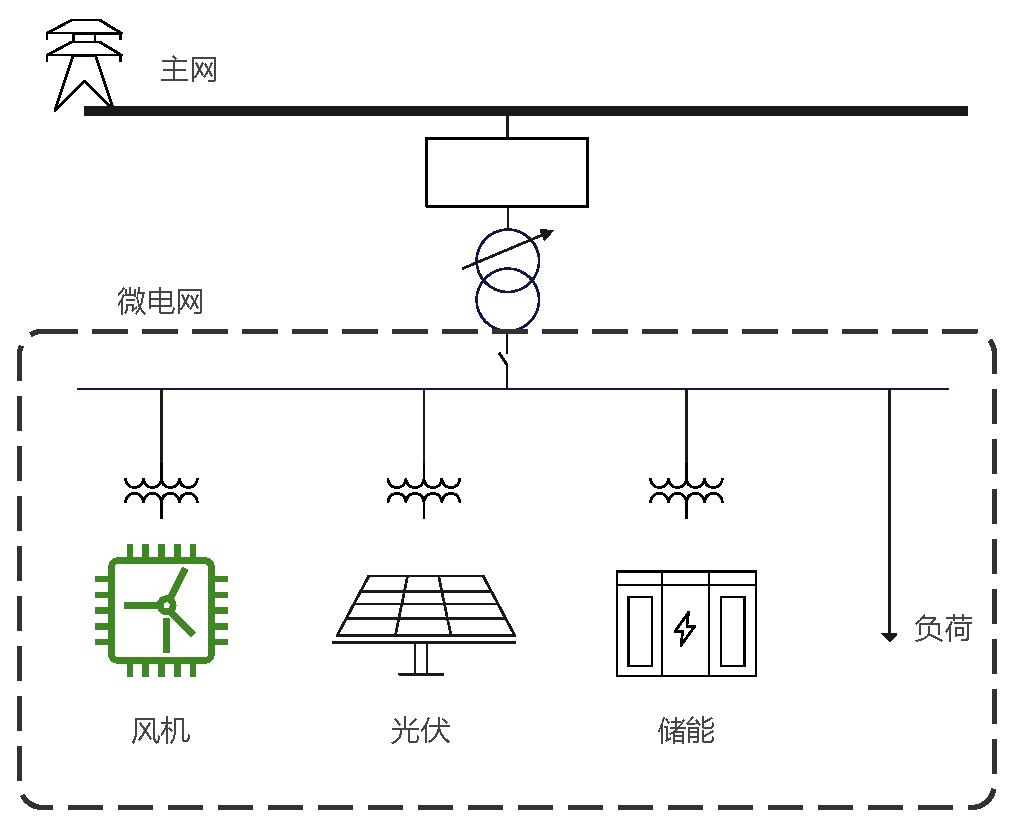
\includegraphics[width=.5\textwidth]{figures/示意图.eps}
\caption{微电网风光储示意图}
\end{figure}

\subsection{问题提出}
\begin{itemize}
\item 问题 1:针对各园区独立运营的情况,首先根据题目给定要求,已知典型日的风光发电功率、风光购电成本、日负荷功率曲线,评估各园区在未配置储能时的运行经济性;其次,配置50kW/100kWh储能后,制定合理的储能运行策略和购电计划,研究运行经济性是否会改善;最后,制定出各园区的最佳储能功率和容量配置方案,并论证该方案的优越性。
\item 问题 2:针对联合园区运营的情况,假设各园区独立实现发电与负荷均衡,首先分析三个园区联合运营但未配置储能时的整体运行经济性;然后,在保持风光荷功率波动特性不变的前提下,制定联合园区的总储能最优配置方案并分析该方案的经济性;最后,分析联合运营所带来的经济收益改变。
\item 问题 3:根据题目所给配置方案条件,制定独立运营、联合运营条件下园区风、光、储能的协调配置方案并分析该方案的经济性;其次根据不同月份的典型日风光发电功率和分时电价,制定独立运营园区的协调配置方案并分析该方案的经济性。
\end{itemize}


\section{问题分析}
\subsection{问题一的分析}
根据题目要求,三个园区的园区负荷与日风光发电功率时序不匹配,通过配置储能系统维持电力系统供需平衡。该问题是一个典型的最小值优化问题。首先,我们分析每个园区的购电量、弃风弃光电量、总供电成本和单位电量平均供电成本,根据不同类型的供电成本占比判断影响经济性的关键因素;接着,计算配置50kW/100kWh储能系统下不同园区的供电成本,包括风电成本、光伏成本、储能成本,在满足储能条件的约束下,制定供电成本最低的充电、放电、购电计划,比较储能前后的经济指标,评估储能系统对经济性的改善效果;最后,假设风光荷功率波动特性保持不变,通过模拟退火算法找到不同园区经济效益最高(即成本最低,弃电最少)配置储能系统。
\subsection{问题二的分析}
在问题一的基础上,假设各园区独立实现发电与负荷均衡将园区联合运营,配置总储能系统。首先,我们分析联合园区的购电量、弃风弃光电量、总供电成本和单位电量平均供电成本,根据不同类型的供电成本占比判断影响经济性的关键因素;然后,根据问题一建立的模型求解最优配置储能系统的充放电功率和储能容量;最后,对比联合园区和独立园区的运行经济性要素,分析导致经济效益改变的主要因素。
\subsection{问题三的分析}
在未来负荷增长的背景下, 园区需要制定风光储协调配置方案, 以满足增加的负荷需求。我们假设各园区的最大负荷增长 $50 \%$, 并且负荷波动特性保持不变。我们首先需要根据各园区的负荷增长和发电数据, 分别制定独立运营和联合运营的风光储协调配置方案。结合全年 12 个月的典型日风光发电功率数据和分时电价策略, 制定购电计划和储能运行策略, 以优化供电成本和提高经济性。通过比较独立运营和联合运营的总供电成本和单位电量平均供电成本, 可以分析各方案的经济性优劣, 并为园区未来的能源规划和投资决策提供科学依据。这种协调配置方案有助于最大化可再生能源的利用效率, 降低总体供电成本, 实现可持续发展目标。


\section{模型假设}
\begin{itemize}
\item 不考虑电能传输过程中的损耗;
\item 该微电网系统的可再生能源发电包括风力发电与光伏发电,此外,该系统还含有蓄电池以及常规负荷。
\item 不考虑配置储能在蓄电池的充、放电过程中的损耗问题,不考虑维修等。
\item 在蓄电池参与调节的单位时间间隔内,充、放电功率保持恒定。
\end{itemize}


\section{符号说明}
\begin{table}[H] % [htbp]是表格位置参数,可根据需要调整    
  \label{tab001} \centering     
  \begin{tabular}{c@{\hspace{6em}}c} % 定义表格列数及对齐方式,这里有两列,都居中对齐    
    \toprule[1.5pt] % 顶部粗线    
    符号   &   意义 \\ % 表格的表头    
    \midrule[1pt] % 中部细线    
    $P_{\text {sum }}(t)$   &   园区在各个时刻的风电、光电发电功率之和 \\
    $P_w(t)$   &   园区在各个时刻的风电发电功率 \\
    $P_s(t)$   &   园区在各个时刻的光伏发电功率 \\    
    $L(t)$   &   园区在各个时刻的日负荷功率 \\     
    $E_{\text {grid }}(t)$   &   园区在各个时刻需要从电网购买的电量。 \\ % 使用$...$来创建数学模式的下角标    
   $E_{\text {discard }}(t)$  &   园区在各个时刻发电量大于负荷时的弃风弃光电量。 \\ % 同上    
    $C_{\text{total}}$   &    总供电成本 \\ % 同上 
    $C_{\text{avg}}$   &   单位电量平均供电成本 \\ 
    $P_{\text {charge }}(t)$   &   储能系统各个时刻的充电量 \\
    $P_{\text {discharge }}(t)$   &   储能系统各个时刻的放电量 \\ 
    $S O C(t)$   &   储能系统各个时刻的荷电状态 \\
    $\eta$   &   充放电效率 \\  
    \bottomrule[1.5pt] % 底部粗线    
  \end{tabular}      
\end{table} 


  \section{模型的建立与求解}  
  \subsection{问题一模型的建立与求解}
  \subsubsection{数据预处理}
  首先读取各园区的典型日负荷数据和风光发电数据,包括负荷数据和风光发电数据。接着,将风光发电数据的标幺值转换为实际功率值,并定义了储能系统的技术参数和成本。
  
\begin{equation}
\begin{aligned}
& P_w(t)=P_{w p u}(t) \times P_{\mathrm{w}} \\
& P_s(t)=P_{s p u} \times P_{\mathrm{pv}}
\end{aligned}
\end{equation}

  
  \subsubsection{未配置储能经济性分析}
  根据题目所给数据,绘出ABC独立园区各个时刻对应的总产电量、负荷电量、向主电网购电量、弃风弃光电量曲线,可以看出AC园区在8时至15时期间发电量大于负荷电量,B园区在0时至5时和17时至19时期间发电量大于负荷电量,存在明显的弃电损失。
  
  \begin{figure}[!h]  
\centering  
\begin{minipage}{.5\textwidth}  
  \centering  
  \includegraphics[width=.9\linewidth]{figures/A.eps}  
  \subcaption{A区示意图}  
\end{minipage}%  
\begin{minipage}{.5\textwidth}  
  \centering  
  \includegraphics[width=.9\linewidth]{figures/B.eps}  
  \subcaption{B区示意图}  
\end{minipage}  
\begin{minipage}{.5\textwidth}  
  \centering  
  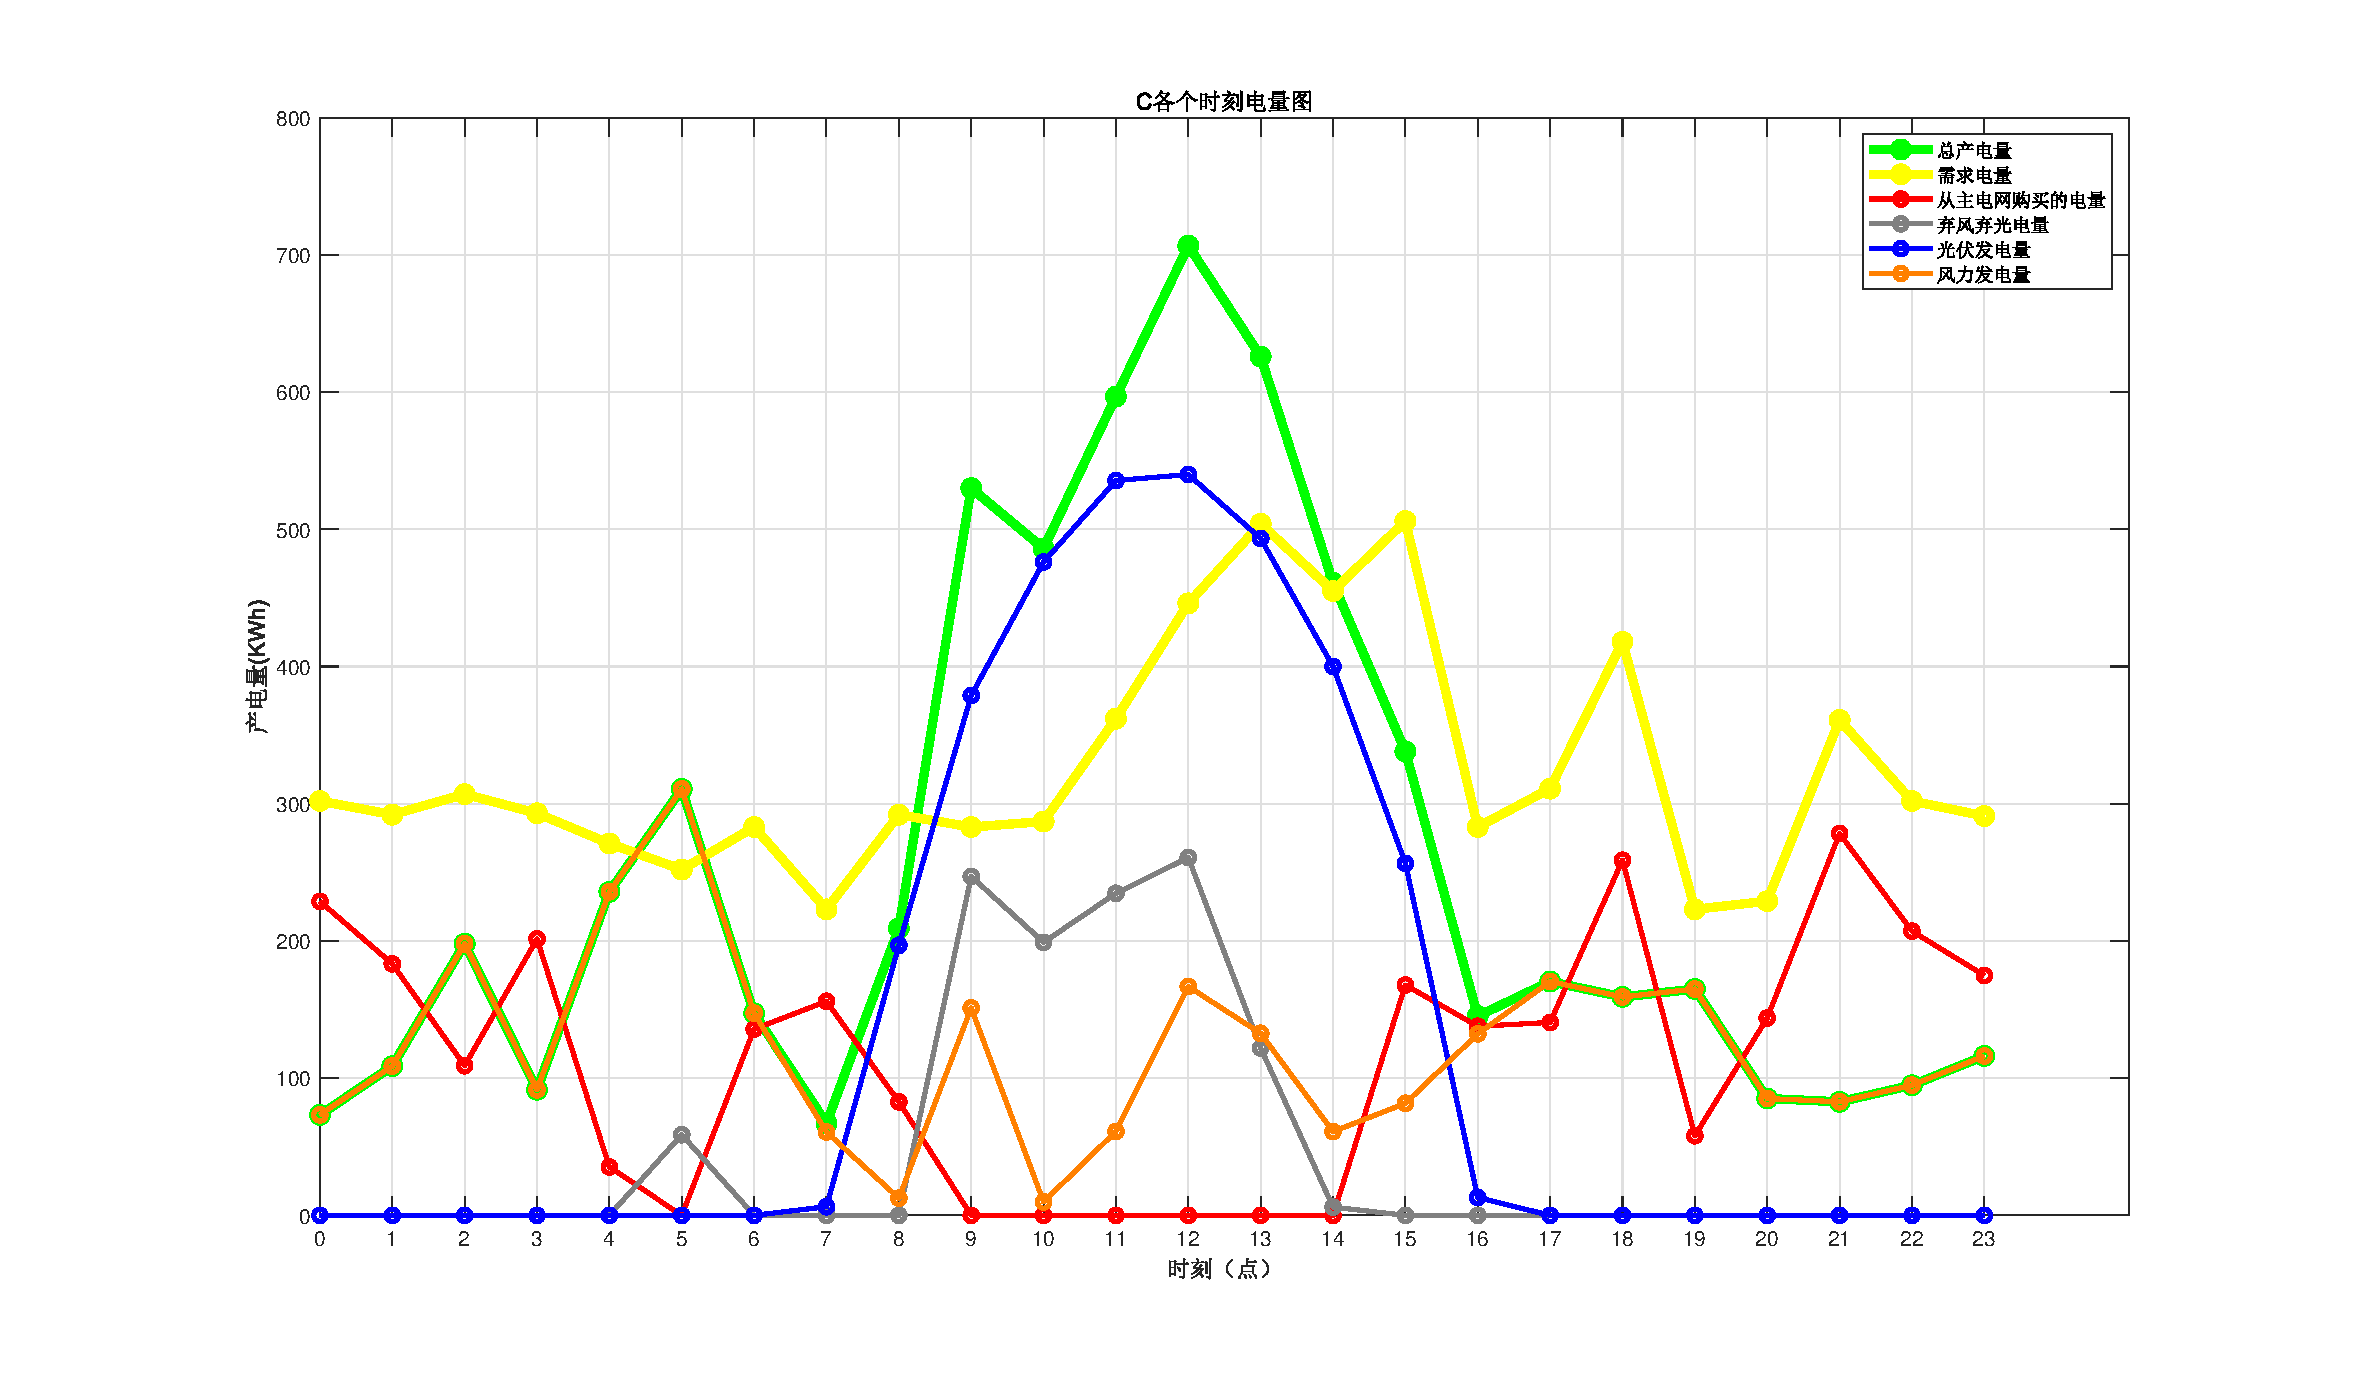
\includegraphics[width=.9\linewidth]{figures/C.eps}  
  \subcaption{C区示意图}  
\end{minipage}  
\caption{各个园区的电量供需对比图}  
\end{figure} 

\newpage

\textbf{弃风弃光电量计算:}
\begin{equation}
E_{\text {discard }}=\sum_{t=1}^{24} \max \left(0, P_{\text {sum }}(t)-L(t)\right)
\end{equation}

\textbf{购电量计算:}

向主电网购电量为:
\begin{equation}
E_{\text{grid}} = \sum_{t=1}^{24} \max \left( 0, L(t) - P_{\text{sum}}(t) \right)
\end{equation}

有效风电发电功率为:
\begin{equation}
P_{w 0}=\max \left\{P_w(t)-E_{\text {discard }}(t), 0\right\}
\end{equation}

有效光电发电功率为:
\begin{equation}
P_{s 0}= \begin{cases}\max \left\{P_s(t)+P_w(t)-E_{\text {discard }}(t), 0\right\}, & P_{w 0}=0 \\ \max \left\{P_s(t), 0\right\}, & P_{w 0} \neq 0\end{cases}
\end{equation}

总购电量=向主电网购电量+风电发电购电量+光电发电购电量,则:
\begin{equation}
E_{\text {sum }}=E_{\text {grid }}+\sum_{t=1}^{24} P_{w 0}(t)+\sum_{t=1}^{24} P_{\text {s0}}(t)
\end{equation}

\textbf{总供电成本计算:}
\begin{equation}
\begin{aligned}
C_{\text {total }} & =C_{W S}+C_{\text {dissard }}+C_{\text {grid }} \\
& =\sum_{t=1}^{24}\left(P_{w 0}(t) w_f+P_{s 0}(t) w_s\right)+E_{\text {grid }} \times w_g
\end{aligned}
\end{equation}


其中,总供电成本计算由风光有效供电成本$C_{FS}$、弃风弃光电成本$C_{\text {dissard }}$、向主电网购电成本$C_{\text {grid }}$三部分构成,$P_{f 0}(t)$和$P_{s 0}(t)$代表有效风电、光电发电功率,$w_f$为风电的单位购电成本,$w_s$为光伏的单位购电成本,$w_g$为电网的单位购电成本。


\textbf{单位电量平均供电成本:}

\begin{equation}
C_{\text {avg }}=\frac{C_{\text {total }}}{\sum_{t=1}^{24} L(t)}
\end{equation}


\textbf{影响其经济性的关键因素分析:}

从表格数据和各个园区的成本饼状图可以看出,ABC园区中,向主电网的购电成本都占园区电费成本的$40 \%$以上,风力、光优购电成本在不同园区的花费占比不同,在 $B C$ 园区可达到 $40 \% \sim 50 \%$,在 $A$ 园区占比小于$25 \%$,园区弃电成本占比最小,小于园区电费成本的 $20 \%$ 。

综上所述,向主电网的购电成本为园区购电成本的的主要因素。结合实际情况,风光发电具有间歇性和波动性的特点,其出力与园区的电力负荷需求往往存在时序上的不匹配,与所求结果相符。

\begin{table}[!h]  
\centering  
\begin{tabular}{|l|l|l|l|l|}  
\hline  
\text{经济要素 }  \text{ (米) } & \text{购电量} & \text{弃风弃光电量} & \text{总供电成本} & \text{单位电量平均供电成本} \\  
\hline  
\text{A园区 }  & 7901.00 & 951.20 & 6084.88 & 0.77  \\  
\hline  
\text{B园区  }  & 7710.00 & 897.50 & 5071.15 & 0.66  \\  
\hline  
\text{C园区  }  & 7776.00 & 1128.02 & 4963.31 &  0.64  \\  
\hline  
\end{tabular}  
\caption{不同园区的经济要素}  
\label{tab:curvature_values}  
\end{table}  

\begin{figure}[!h]  
\centering  
\begin{minipage}{.5\textwidth}  
  \centering  
  \includegraphics[width=.9\linewidth]{figures/A饼图.pdf}  
  \subcaption{A区示意图}  
\end{minipage}%  
\begin{minipage}{.5\textwidth}  
  \centering  
  \includegraphics[width=.9\linewidth]{figures/B饼图.jpg}  
  \subcaption{B区示意图}  
\end{minipage}  
\begin{minipage}{.5\textwidth}  
  \centering  
  \includegraphics[width=.9\linewidth]{figures/C饼图.pdf}  
  \subcaption{C区示意图}  
\end{minipage}  
\caption{各个园区的成本饼状图}  
\end{figure} 

\newpage




  \subsubsection{储能运行与购电模型}\label{ll}
针对第二小问,需要对配置了50kW/100kWh储能系统的三个园区制定最优运行策略及购电计划。我们的目标是通过合理地管理储能系统的充放电过程,以最小化园区的总成本和减少弃风弃光现象。

首先根据风光发电数据和负荷需求来确定储能系统的充放电策略。具体来说,当风光发电量大于负荷需求时,我们将多余的电量优先用于给储能系统充电,以确保其能够在未来需要时释放能量。

在这个过程中,我们需要同时考虑储能系统的最大充放电功率$P_{\text {max}}$和储能容量的限制($S O C_{\text {min }}$至$S O C_{\text {max }}$)。如果风光发电量过多,导致储能系统达到最大容量($S O C_{\text {max }} \times P_{\text {max}}$)后仍有剩余电量,我们将计算并记录这部分被丢弃的风光发电量。

\vspace{1cm}

\textbf{决策变量:}

我们首先定义了一组决策变量,用来描述系统的充放电策略和购电计划:

第 $t$ 时段从电网购电量为 $E_{\text {grid }}(t)$

第 $t$ 时段充风弃光电量为 $E_{\text {discard }}(t)$

第 $t$ 时段系统的充电量为 $P_{\text {charge }}(t)$

第 $t$ 时段系统的放电量为 $P_{\text {discharge }}(t)$


由于风电购电成本高于光伏发电成本 $w_f>w_s$ ,故有效风电发电功率为:
\begin{equation}
P_{w 0}=\max \left\{P_w(t)-E_{\text {discard }}(t), 0\right\}
\end{equation}

有效光伏发电功率为:
\begin{equation}
P_{s 0}= \begin{cases}\max \left\{P_s(t)+P_w(t)-E_{\text {discard }}(t), 0\right\}, & P_{w 0}=0 \\ \max \left\{P_s(t), 0\right\}, & P_{w 0} \neq 0\end{cases}
\end{equation}

\textbf{目标函数:}

总供电成本:
\begin{equation}
C_{\text {total }}=\sum_{t=1}^{24}\left(E_{\text {grid }}(t) \cdot w_g+P_{w 0}(t) w_f+P_{s 0}(t) w_s\right)+C_{\text {day }}
\end{equation}

根据储能系统配置,电池最大充放电功率为$P_{\max }$,最大储能容量为$E_{\max }$,则储能系统投资日成本为:
$$
C_{\text {day }}=\frac{P_{\max } \times 800+E_{\max } \times 1800}{360 \times 10}=60.27 
$$

单位电量供电成本:
\begin{equation}
C_{a v g}=\frac{C_{\text {total }}}{\sum_t L(t)}
\end{equation}

\textbf{约束条件:}

购电量约束: 如果储能系统放电不足,则购电补充:
\begin{equation}
\left.E_{\text {grid }}(t)=\max \left\{L(t)-P_{\text {sum }}(t)-P_{\text {discharge }}(t), 0\right)\right\}
\end{equation}

弃风弃光电量约束: 如果储能系统充电已达上限,则弃风弃光: 
\begin{equation}
\left.E_{\text {discard }}(t)=\max \left\{P_{\text {sum }}(t)-L(t)-P_{\text {charge }}(t), 0\right)\right\}
\end{equation}

充放电状态约束:
\begin{equation}
P_{\text {discharge }}(t) P_{charge}(t)=0
\end{equation}

根据题目所给条件,设储能系统荷电初始状态为$S O C\left(t_0\right)=10 \%$,根据充放电机制:
\begin{equation}
S O C(t+1)=S O C(t)+\frac{\eta \cdot P_{\text {charge }}(t)-P_{\text {discharge }}(t) / \eta}{E_{\text {max }}}
\end{equation}


约束条件为:
\begin{equation}
\begin{gathered}
S O C_{\text {min }} \leq S O C(t) \leq S O C_{\text {max }} \\
0 \leq P_{\text {charge }}(t), P_{\text {discharge }}(t) \leq P_{\max } \\
E_{\text {grid }}(t) \geq 0
\end{gathered}
\end{equation}

功率平衡约束为:
\begin{equation}
L(t)=P_{\text {gen }}(t)+P_{\text {discharge }}(t)-P_{\text {charge }}(t)+E_{\text {grid }}(t)
\end{equation}


\textbf{模型求解} 
 
当风光发电量大于负荷需求时,我们将多余的电量优先用于给储能系统充电,以确保其能够在未来需要时释放能量;当风光发电量小于负荷需求时,我们优先用储能系统放电为电网提供能量,如果无法达到负荷,则向主电网购电,以确保储能系统的充分利用。


求解结果如下:
\begin{figure}[!h]  
\centering  
\begin{minipage}{.5\textwidth}  
  \centering  
  \includegraphics[width=.9\linewidth]{figures/1_2_A.eps}  
  \subcaption{A园区供电示意图}  
\end{minipage}%  
\begin{minipage}{.5\textwidth}  
  \centering  
  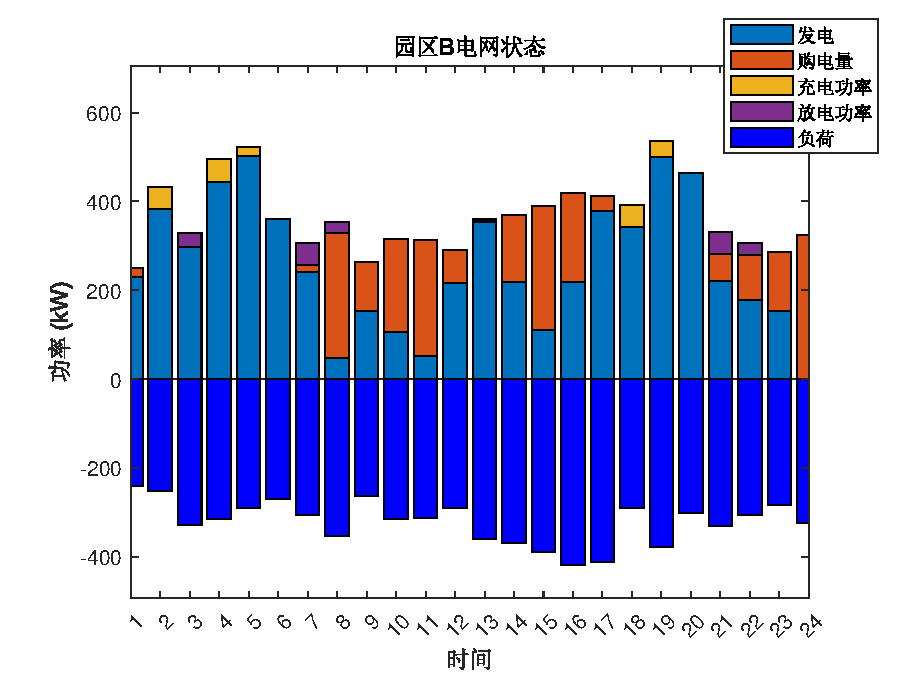
\includegraphics[width=.9\linewidth]{figures/1_2_B.eps}  
  \subcaption{B园区供电示意图}  
\end{minipage}  
\begin{minipage}{.5\textwidth}  
  \centering  
  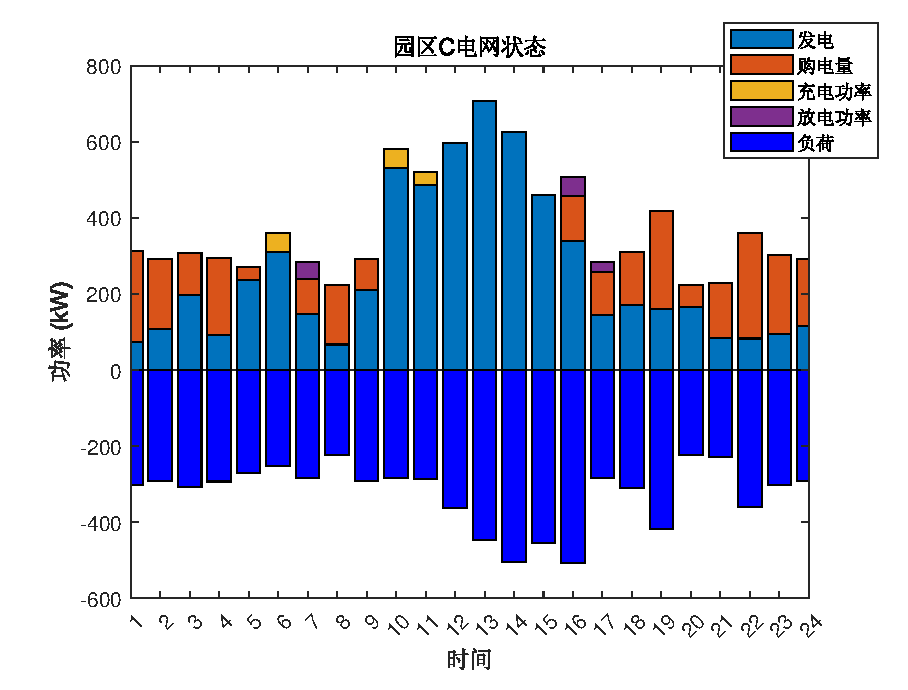
\includegraphics[width=.9\linewidth]{figures/1_2_C.eps}  
  \subcaption{C园区供电示意图}  
\end{minipage}  
\caption{各个园区供电示意图}  
\end{figure} 

园区A充电时间段为10时、11时,充电功率$\text{ (kWh) }$为50.00、34.21;放电时间段为16时、17时,功率$\text{ (kWh) }$为50.00、26.00;

园区B充电时间段为2时、4时、5时、18时、19时,充电功率$\text{ (kWh) }$为50.00、50.00、19.89、50.00、34.21;放电时间段为3时、7时、8时、21时、122时,功率$\text{ (kWh) }$为32.20、50.00、26.00、50.00、26.00;

园区C充电时间段为6时、10时、11时,充电功率$\text{ (kWh) }$为50.00、50.00、34.21;放电时间段为7时、16时、17时,功率$\text{ (kWh) }$为45.13、50.00、26.00;

\newpage

\newpage

\textbf{经济性前后对比} 

\begin{figure}[!h]  
\centering  
\begin{minipage}{.5\textwidth}  
  \centering  
  \includegraphics[width=.9\linewidth]{figures/1_2_A2比较.eps}  
  \subcaption{A区储能前后供电成本对比图}  
\end{minipage}%  
\begin{minipage}{.5\textwidth}  
  \centering  
  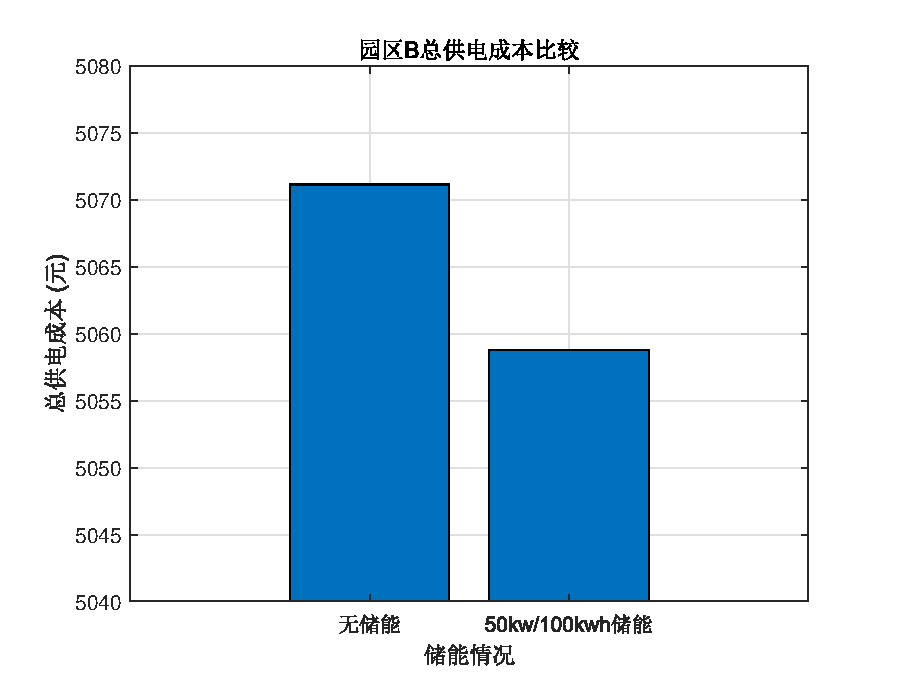
\includegraphics[width=.9\linewidth]{figures/1_2_B2比较.eps}  
  \subcaption{B区储能前后供电成本对比图}  
\end{minipage}  
\begin{minipage}{.5\textwidth}  
  \centering  
  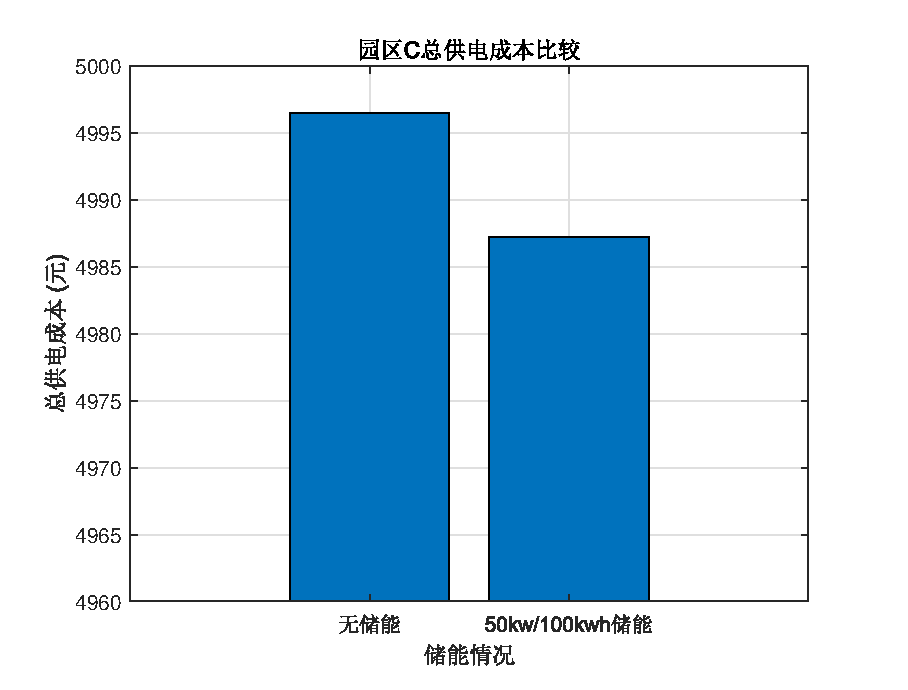
\includegraphics[width=.9\linewidth]{figures/1_2_C2比较.eps}  
  \subcaption{C区储能前后供电成本对比图}  
\end{minipage}  
\caption{各个园区储能前后供电成本对比图}  
\end{figure} 

从下图不同园区储能前后供电成本对比图可以看出,配置50kW/100kWh储能后,各园区的总供电成本改变,其中A园区的总供电成本由6084.88元增大至6112.33元,B园区由5071.15元减少至5058.77元,C园区由4996.48元减少至4987.23元。

结合各个园区的示意图,可以明显看出,A园区的发电功率只在10时、11时大于负荷功率,充电时长短、充电量少,无法充分利用储能装置,故总供电成本增加;而BC园区充放电时长较长,充放电量较大,充分利用储能装置,故总供电成本减少。

\textbf{原因分析:}

在微网系统中,引入蓄电池技术后,全天供电费用相较于仅依赖可再生能源全额利用时有所降低。这种费用减少的主要原因在于,蓄电池有效地解决了可再生能源发电过程中产生的“过剩”电能问题。在可再生能源发电高峰期,这些无法即时消纳的电能可以被蓄电池储存起来。随后,在可再生能源发电量不足以支撑负荷需求时,蓄电池能够释放储存的电能,为微网提供必要的电力支持。通过这种方式,微网系统能够减少对主网的依赖,避免在能源短缺时购买昂贵的外部电力,从而显著提升了微网的经济运行效率。同时,由于减少了向主网的购电量,平均购电单价也相应下降。
  
\subsubsection{储能配置模型}

\textbf{模型建立}  

根据题目要求,我们将需要分别考虑每个园区的风光发电特性、负荷曲战以及储能系统的运行约束,从而制定出合理的储能运行策略和购电计划,最终实现运营成本的最小化。

为了解决这一优化问题,我们在上一问的最小总供电成本模型的基础上,将储能系统的功率$P_{\max }$和容量$E_{\max }$设为变量,该模型的基本思路如下:

第一阶段:确定储能系统的容量配置,即确定储能系统的功率和容量。

设电池充放电最大功率为$P_{\max }$,储能额定容量$E_{\max }$,则电池系统的电成本$C_{\text {year }}$为:
\begin{equation}
C_{\text {year }}=P_{\max } \times 800+E_{\max } \times 1800
\end{equation}
电池储能系统(寿命以十年计)的日成本为:
\begin{equation}
C_{\text {day }}=\frac{C_{\text {year }}}{3650}
\end{equation}

第二阶段:根据第一阶段确定的储能容量,制定每一个决策时段(如每天)的储能运行策略和购电计划,从而最小化该时段的运营成本。

充电和放电过程中 SOC 的更新公式(与第二小问相同)为:
\begin{equation}
S O C(t+1)=S O C(t)+\frac{\eta \cdot P_{\text {charge }}(t)-P_{\text {discharge }}(t) / \eta}{E_{\max }}
\end{equation}

根据上一问的模型,总供电成本为:
\begin{equation}
C_{\text {total }}=\sum_{t=1}^{24}\left(E_{\text {grid }}(t) \cdot w_g+P_{w 0}(t) w_f+P_{s 0}(t) w_s\right)+C_{\text {day }}
\end{equation}

根据查阅资料发现应满足新增电池容量值约束条件, 确保其在合理范围内:
$$
1.5 P_{\max } \leq E_{\max } \leq 3 P_{\max }
$$

  
\textbf{模型求解}

该模型为典型的最小值优化问题,为使总供电成本$C_{\text {total }}$最小,找到最优的$P_{\max }$ 和 $E_{\max }$,采用模拟退火算法进行求解,具体思路如下:

\begin{minipage}{0.5\textwidth} % 左侧文本宽度设置为0.5\textwidth  
  
% 在这里输入你的文字  
1. 初始化 $\left(P_{\max }, E_{\max }\right), T, \alpha$  
  
2. 计算初始解的成本 $C_{\text {current }}$  
  
3. 重复以下步骤直到满足终止条件:  
  
\begin{enumerate}  
    \item 在邻域内生成新解 $\left(P_{\text {new }}, E_{\text {new }}\right)$  
    \item 计算新解的成本 $C_{\text {new }}$  
    \item 计算接受概率 $P$  
    \item 按照接受概率决定是否接受新解  
    \item 更新当前解和当前成本  
    \item 按照降温速率更新温度 $T$  
\end{enumerate}  
  
4. 输出最优解及其对应的最小成本  
  
\end{minipage}  
\hfill % \hfill用于填充空白,使得minipage尽可能靠右  
\begin{minipage}{0.45\textwidth} % 右侧图片宽度设置为0.45\textwidth(稍微小于0.5以留出空白)  
  
\centering  
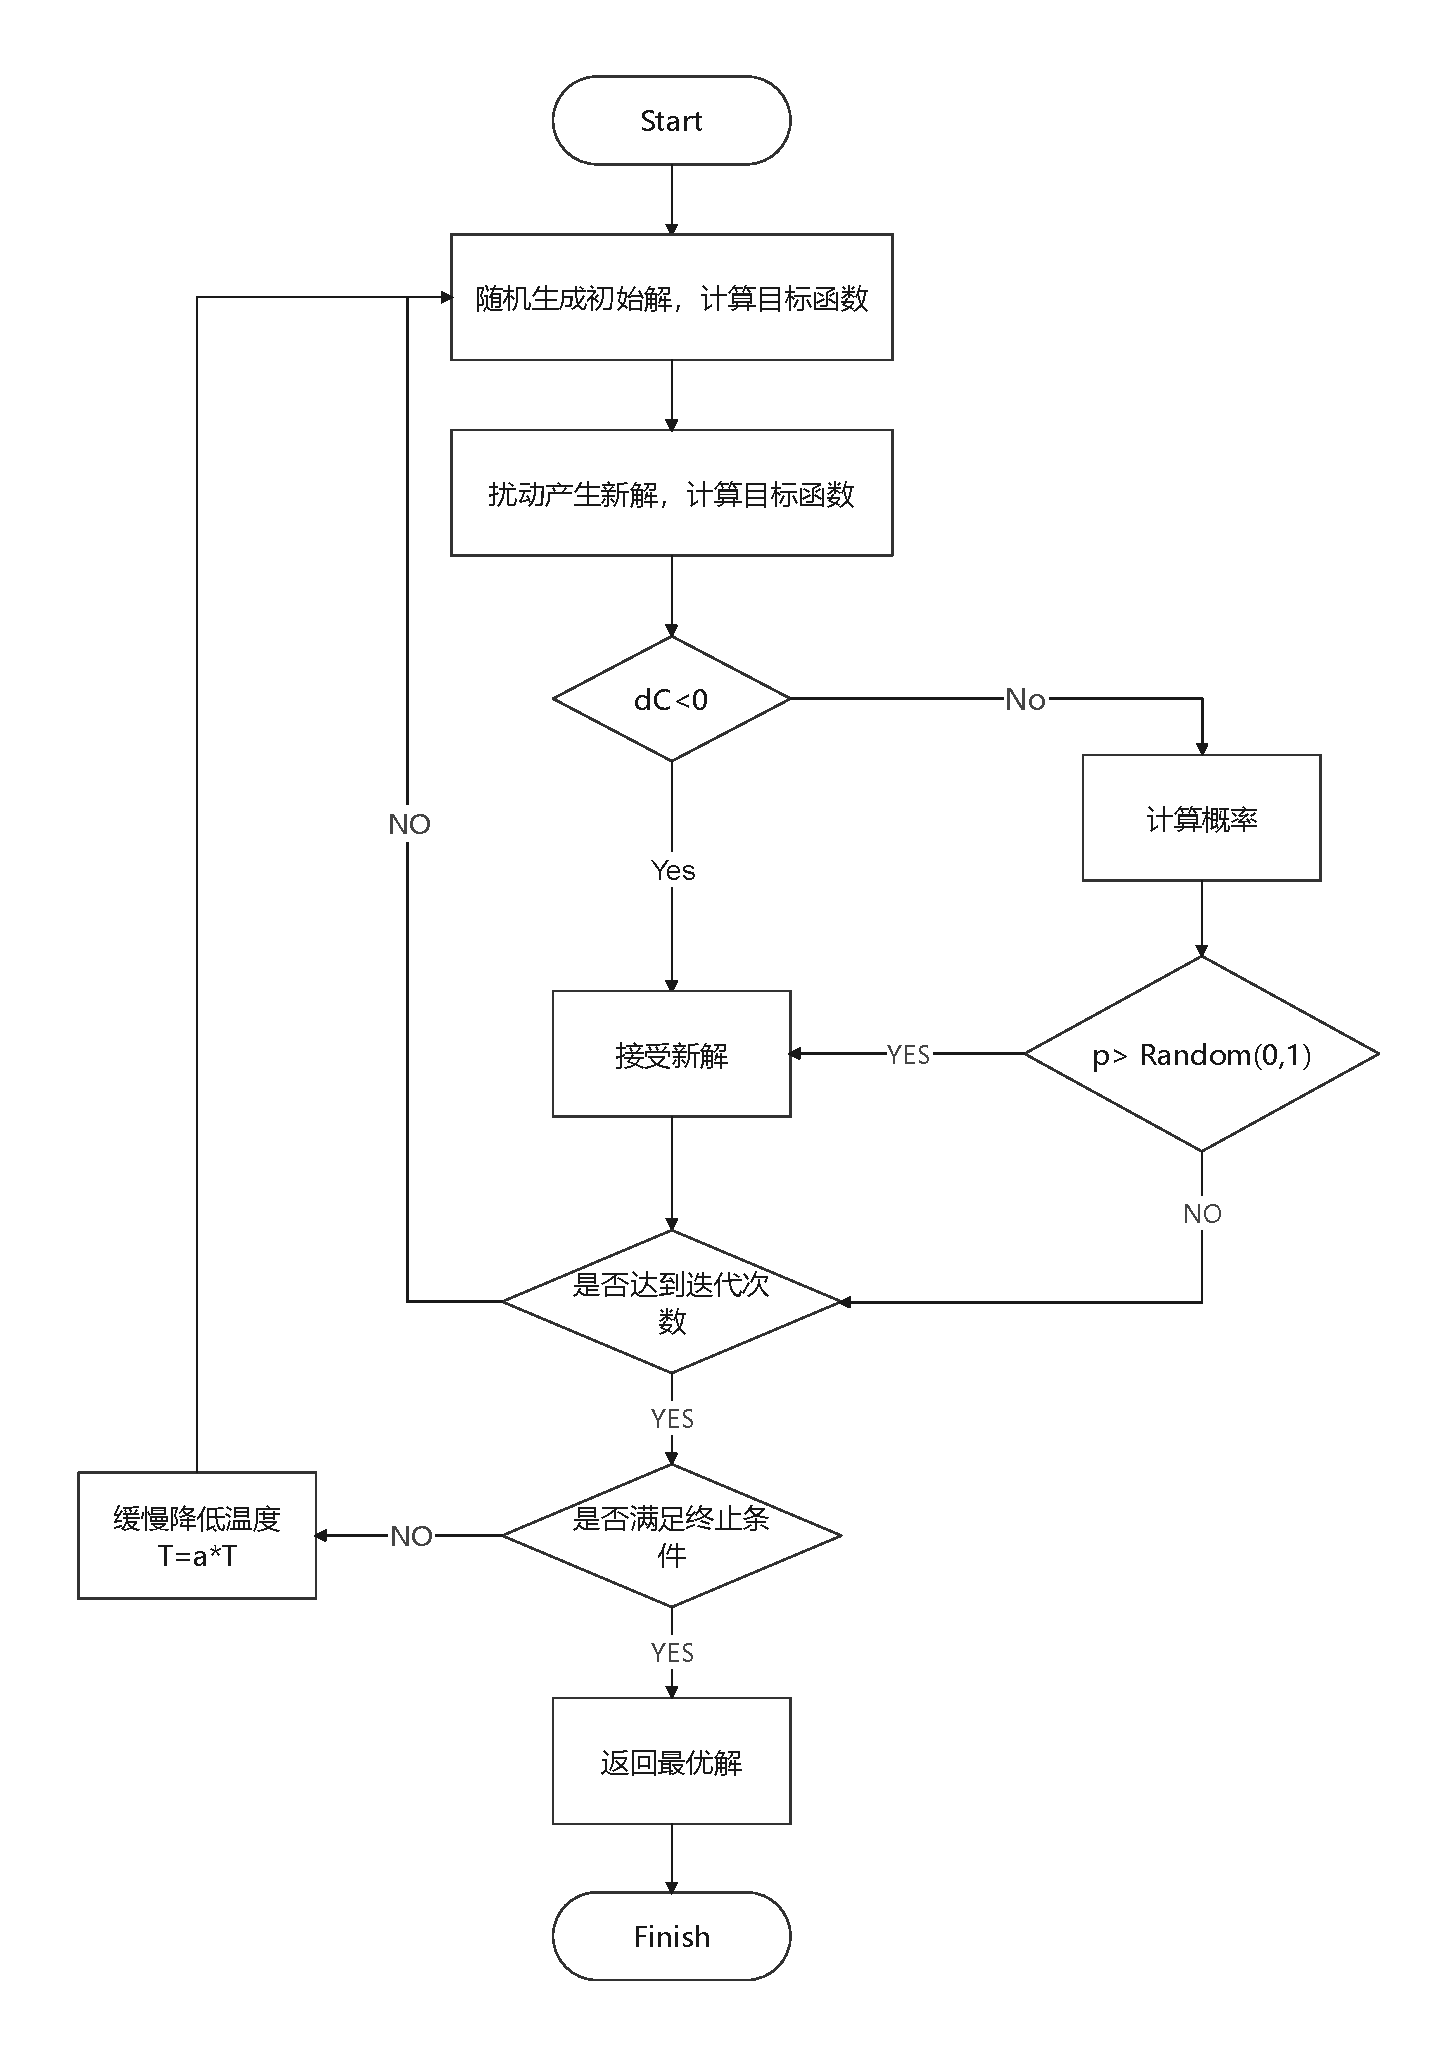
\includegraphics[width=\textwidth]{figures/退火.eps} % 假设你的图片名为"退火.eps"  
\captionof{figure}{模拟退火算法示意图} % 使用captionof来在minipage中提供caption  
  
\end{minipage}  


\textbf{求解结果:}

根据模拟退火算法求解出各园区最优的储能功率、容量配置方案如下图表所示:

  \begin{figure}[!h]  
\centering 
\begin{minipage}{.5\textwidth}  
  \centering  
  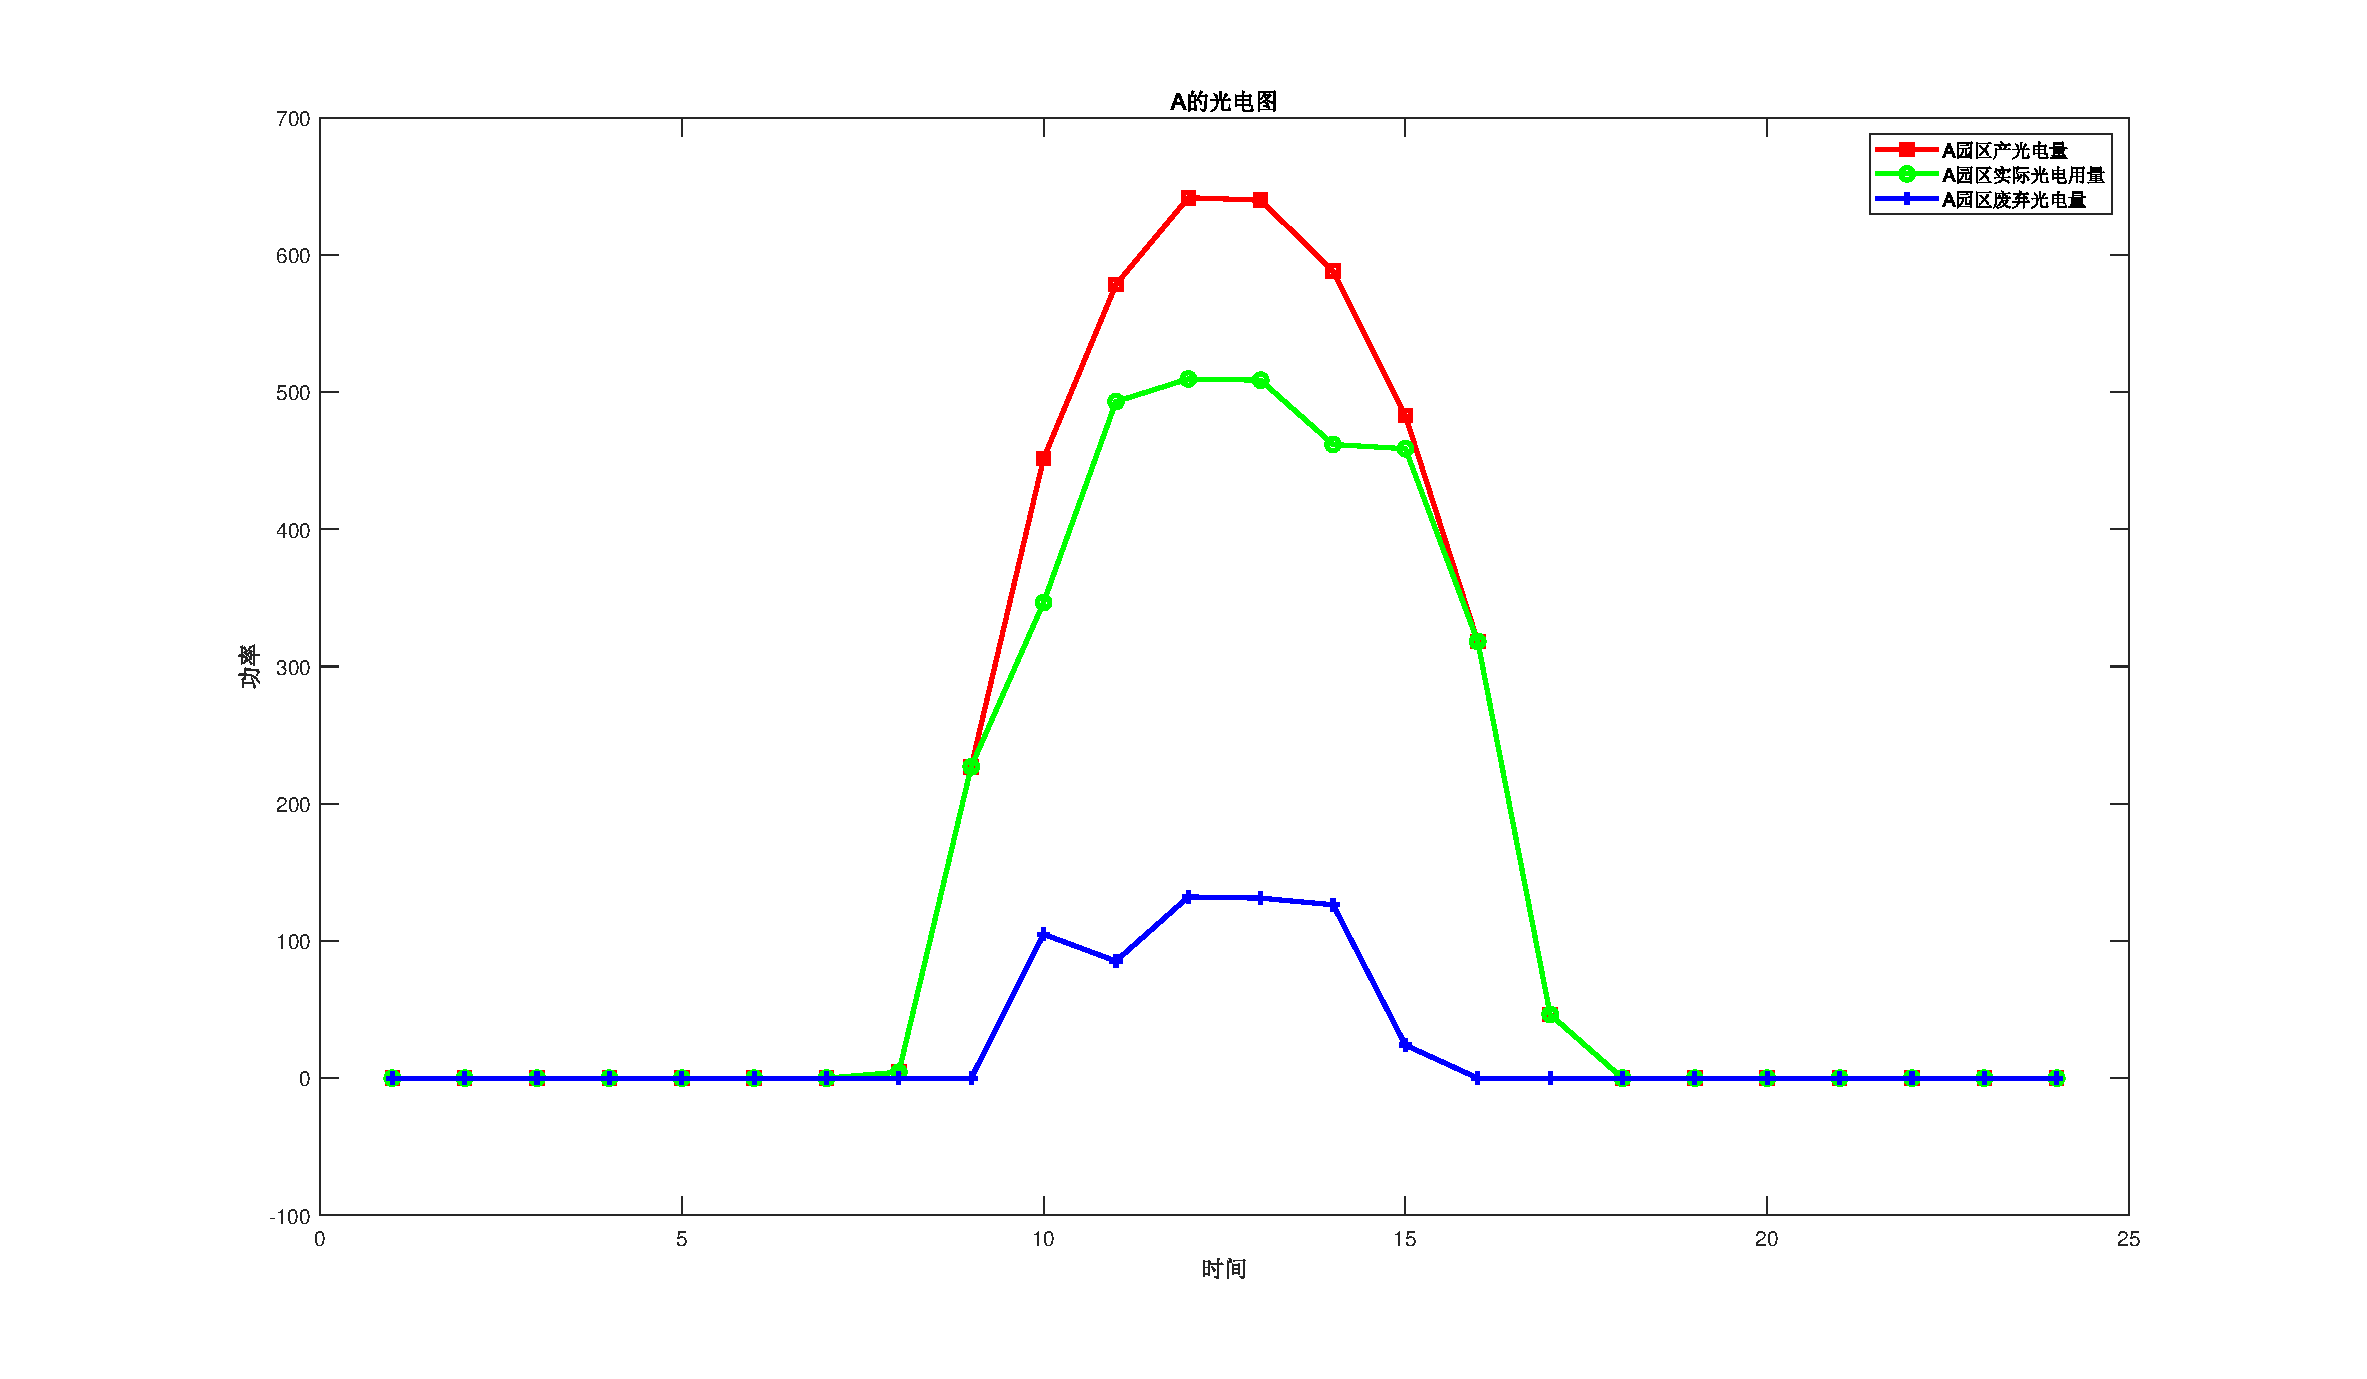
\includegraphics[width=.9\linewidth]{figures/Q1_3_A_light.eps}  
  \subcaption{A区有效光电发电量图}  
\end{minipage}%  
\begin{minipage}{.5\textwidth}  
  \centering  
  \includegraphics[width=.9\linewidth]{figures/Q1_3_A_SOC.eps}  
  \subcaption{A区SOC结果图}  
\end{minipage}  
\begin{minipage}{.5\textwidth}  
  \centering  
  \includegraphics[width=.9\linewidth]{figures/Q1_3_A_sort.eps}  
  \subcaption{A园区的电量供需对比图}  
\end{minipage}
\caption{A园区}  
   
\end{figure} 

  \begin{figure}[!h]  
\centering 
\begin{minipage}{.5\textwidth}  
  \centering  
  \includegraphics[width=.9\linewidth]{figures/Q1_3_B_wind.eps}  
  \subcaption{B区有效风电发电量图}  
\end{minipage}%  
\begin{minipage}{.5\textwidth}  
  \centering  
  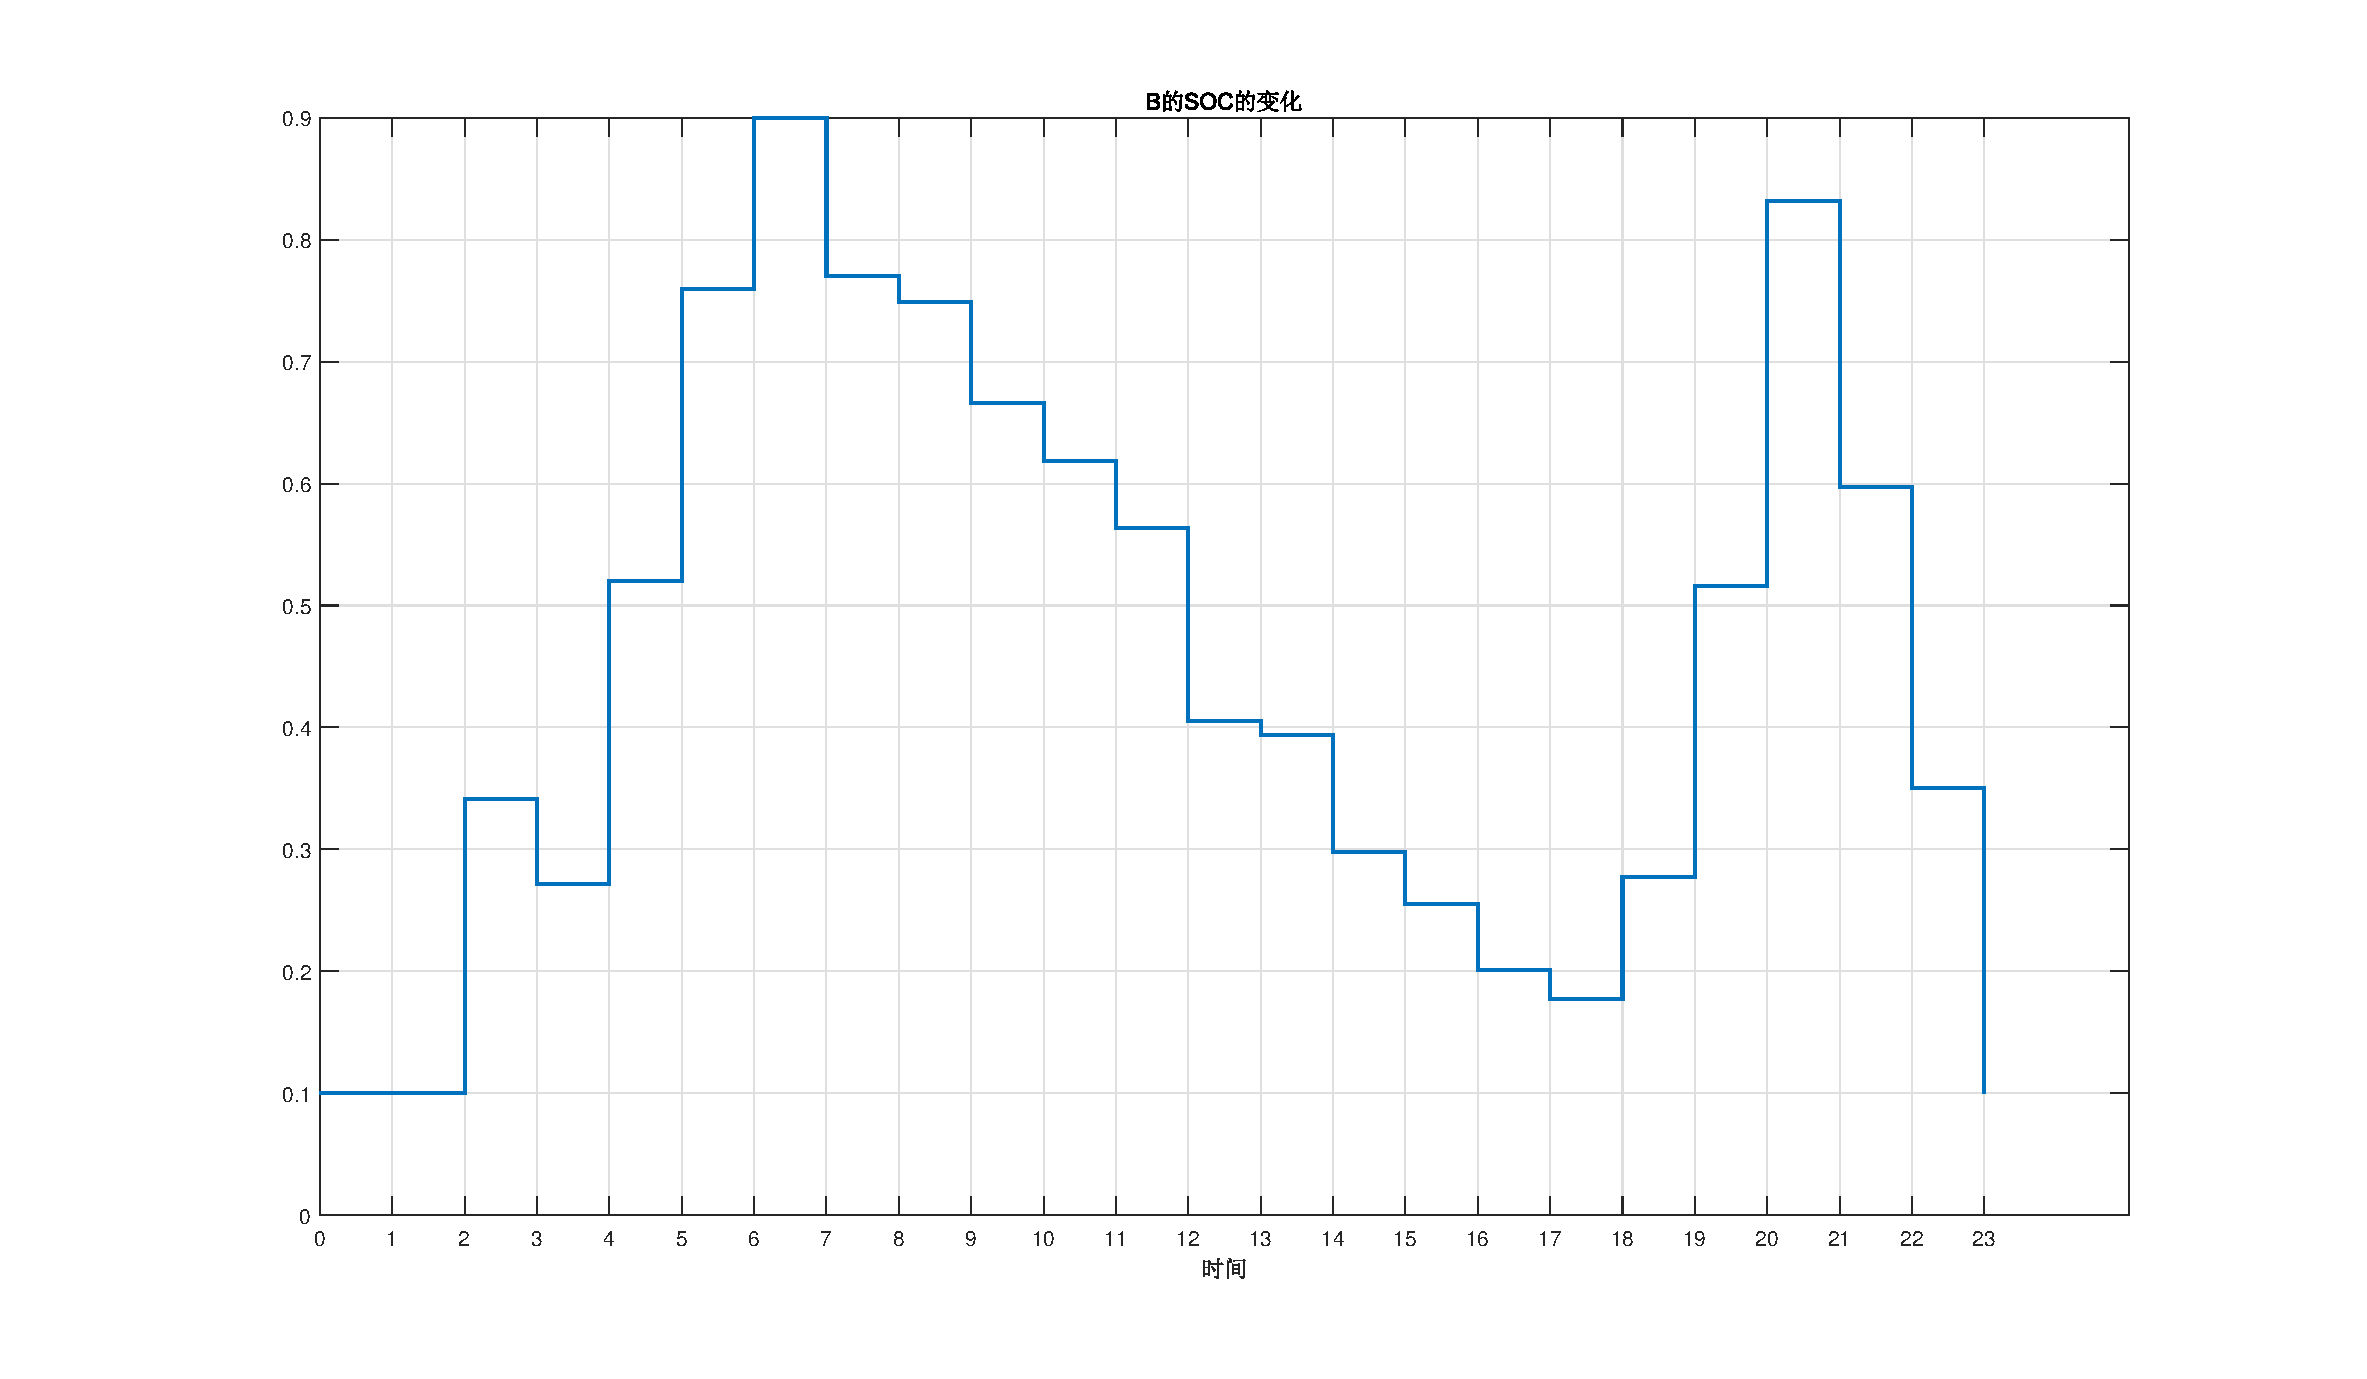
\includegraphics[width=.9\linewidth]{figures/Q1_3_B_SOC.eps}  
  \subcaption{B区SOC结果图}  
\end{minipage}  
\begin{minipage}{.5\textwidth}  
  \centering  
  \includegraphics[width=.9\linewidth]{figures/Q1_3_B_sort.eps}  
  \subcaption{B园区的电量供需对比图}  
\end{minipage}  
\caption{B园区}  
\end{figure} 

\begin{figure}[!h]  
\centering  
\begin{minipage}{.5\textwidth}  
  \centering  
  \includegraphics[width=.9\linewidth]{figures/Q1_3_C_wind.eps}  
  \subcaption{C区有效风电发电量图}  
\end{minipage}%  
\begin{minipage}{.5\textwidth}  
  \centering  
  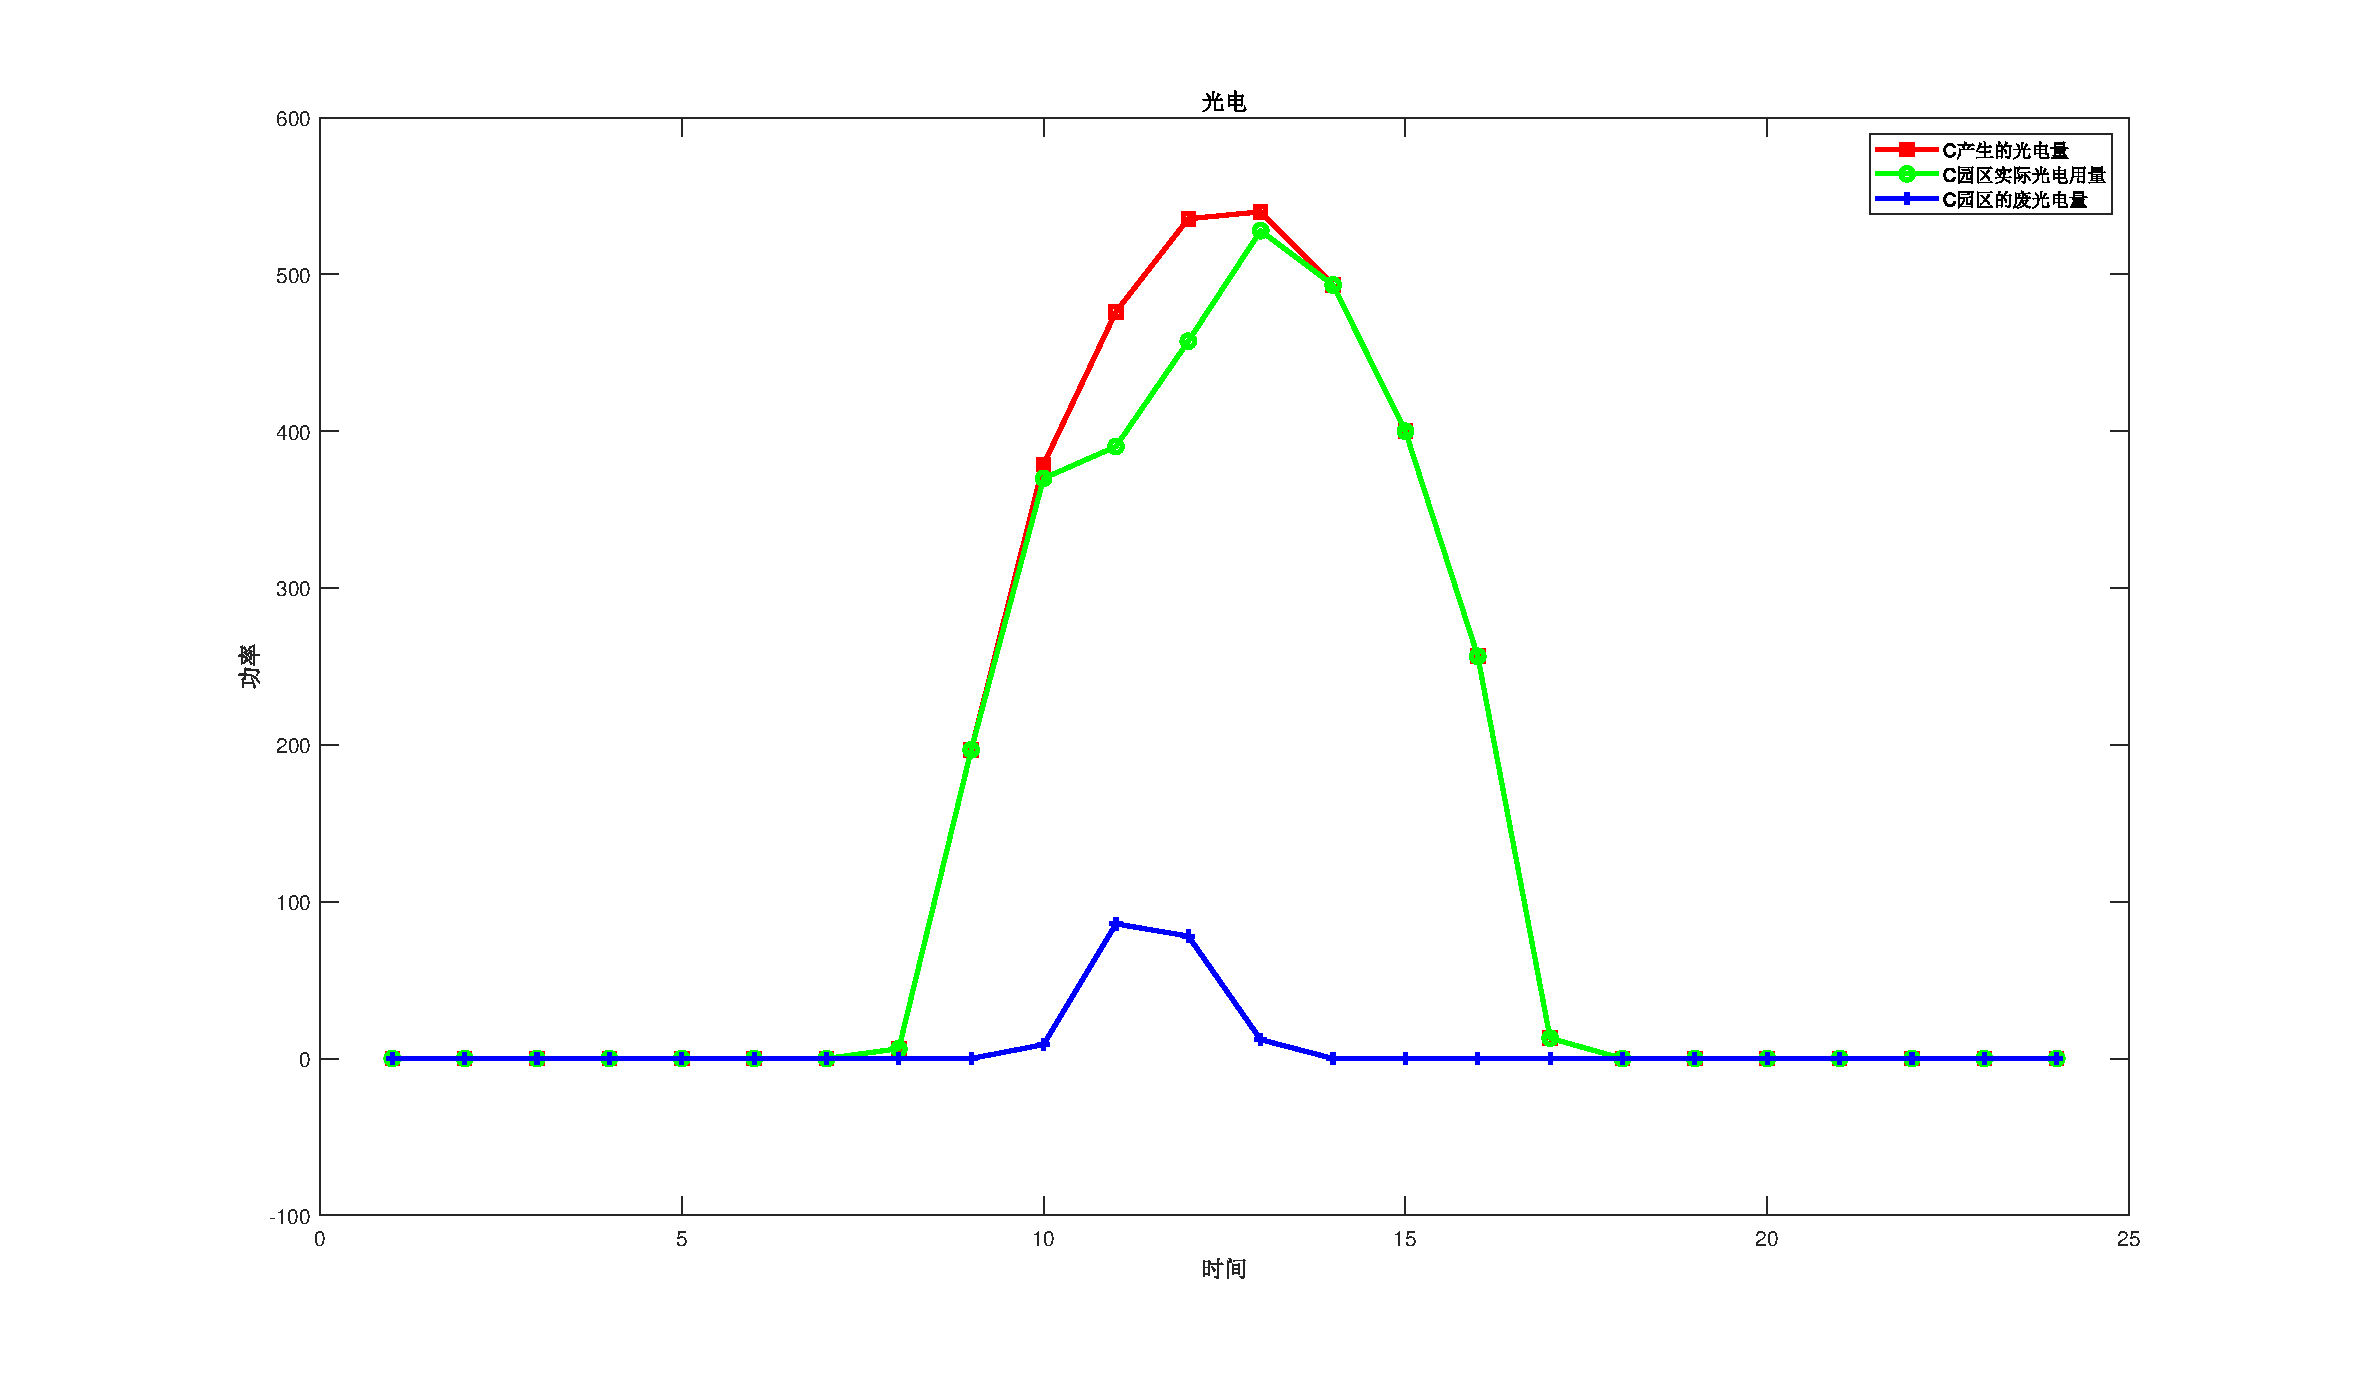
\includegraphics[width=.9\linewidth]{figures/Q1_3_C_light.eps}  
  \subcaption{C区有效光电发电量图}  
\end{minipage}  
  
\par\medskip % 添加一些垂直间距  
  
\begin{minipage}{.5\textwidth}  
  \centering  
  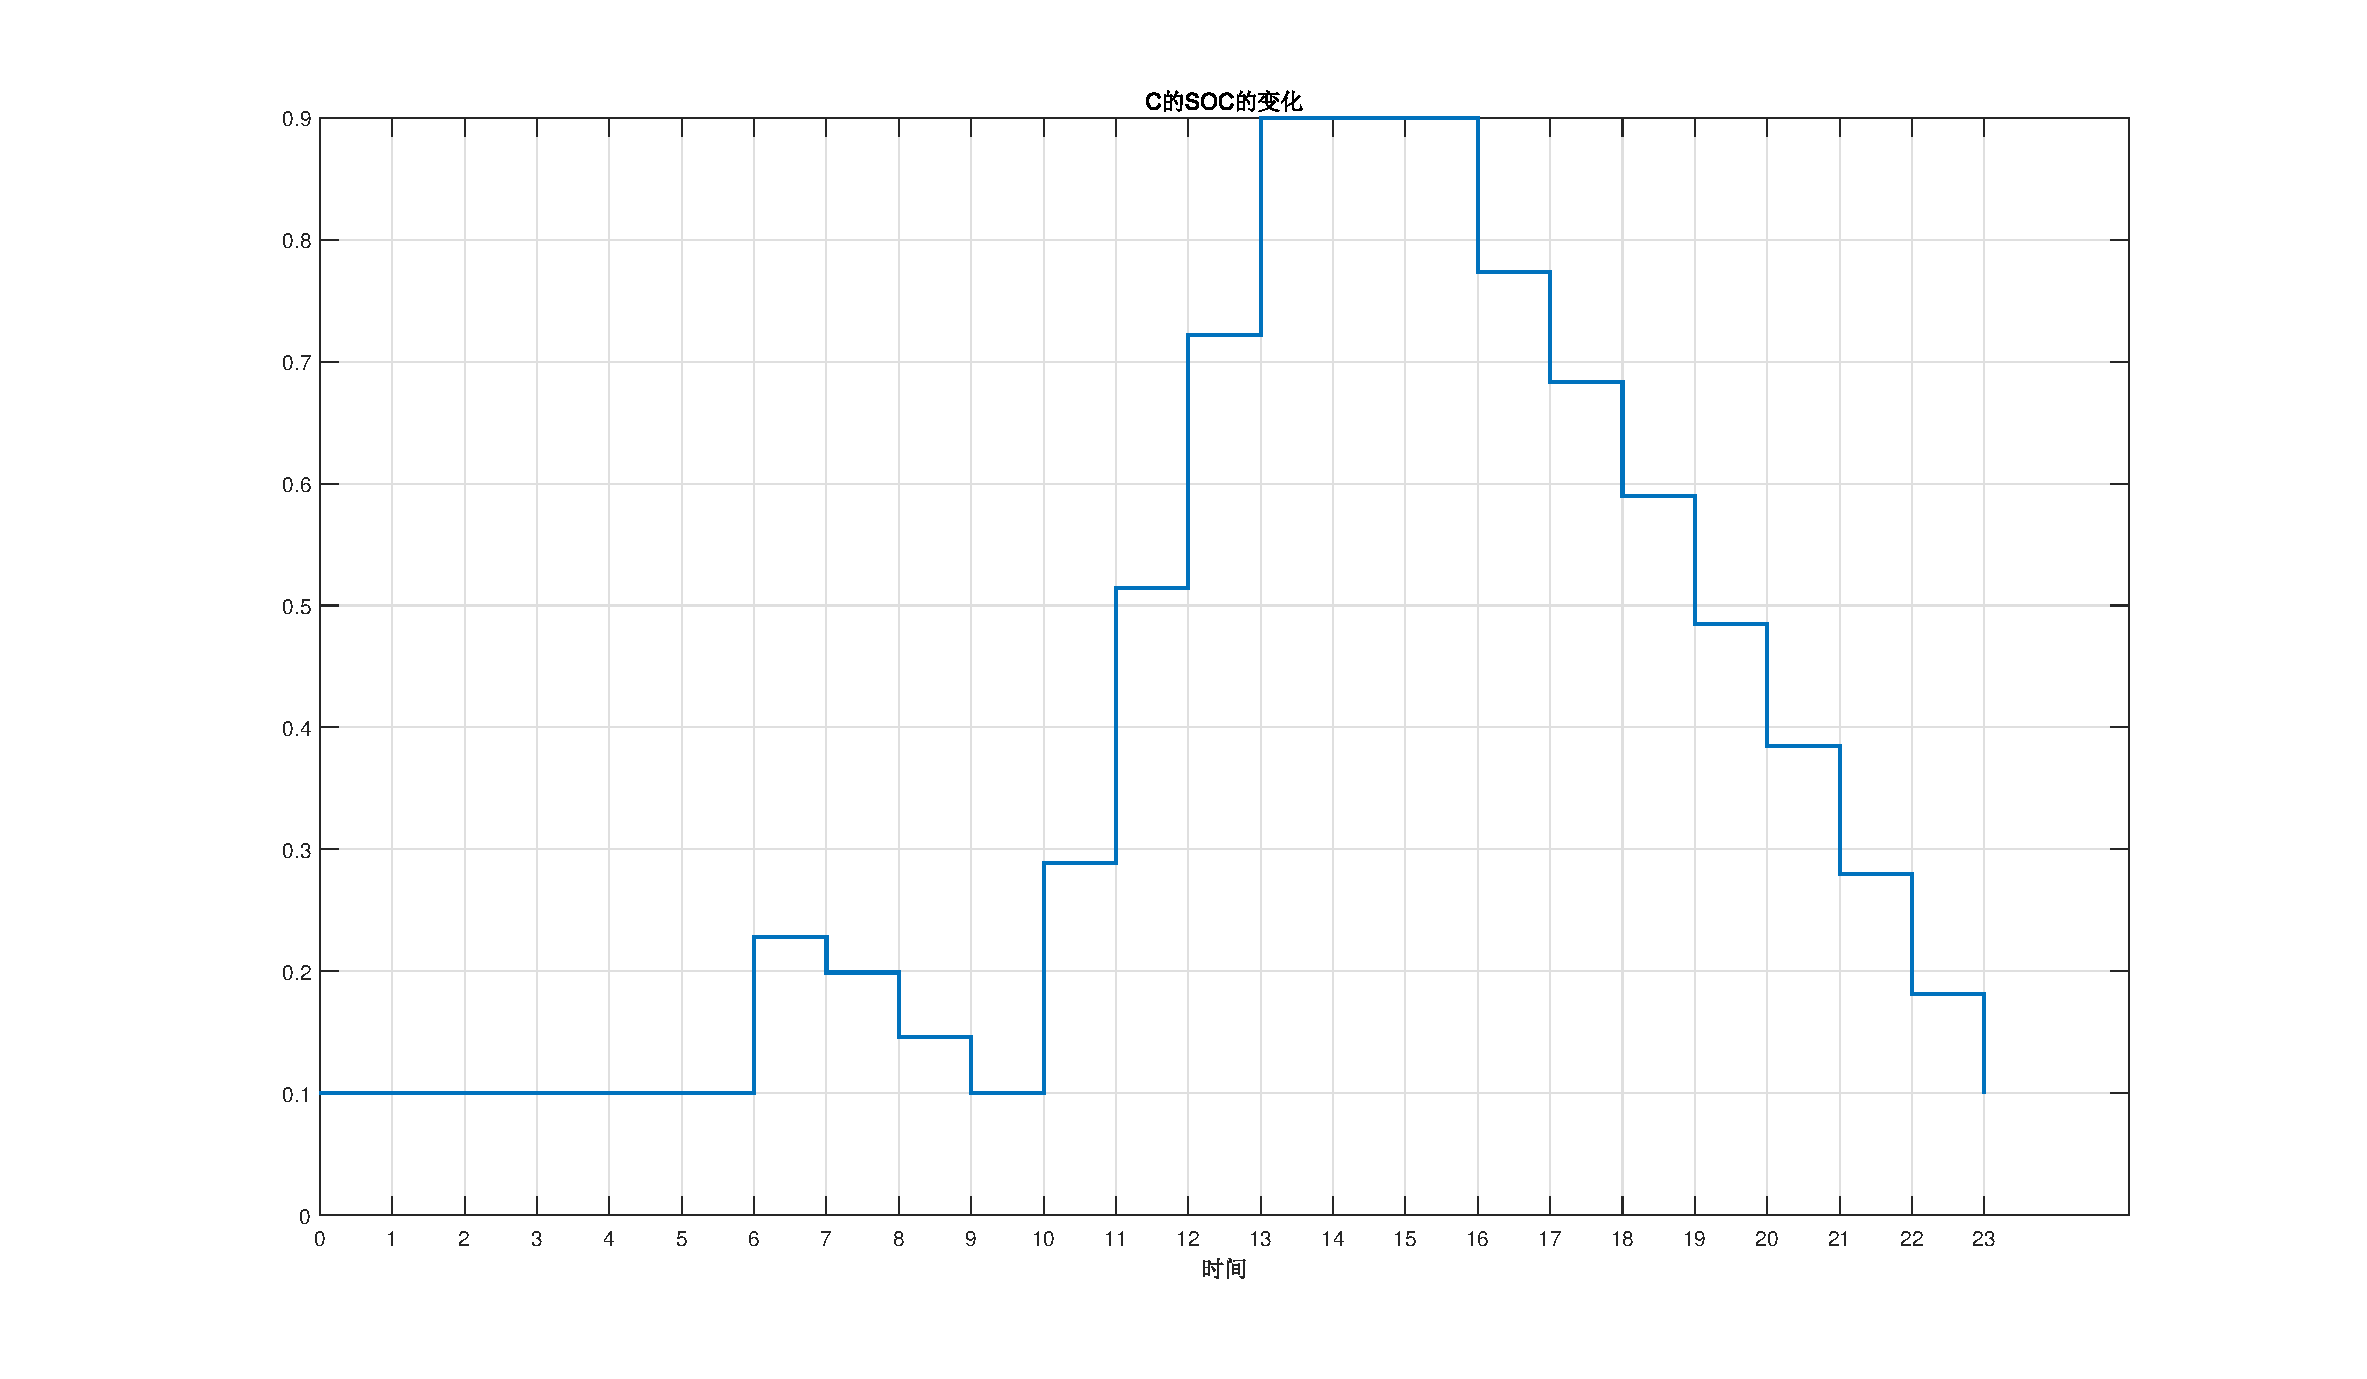
\includegraphics[width=.9\linewidth]{figures/Q1_3_C_SOC.eps}  
  \subcaption{C区SOC结果图} 
\end{minipage}%  
\begin{minipage}{.5\textwidth}  
  \centering  
  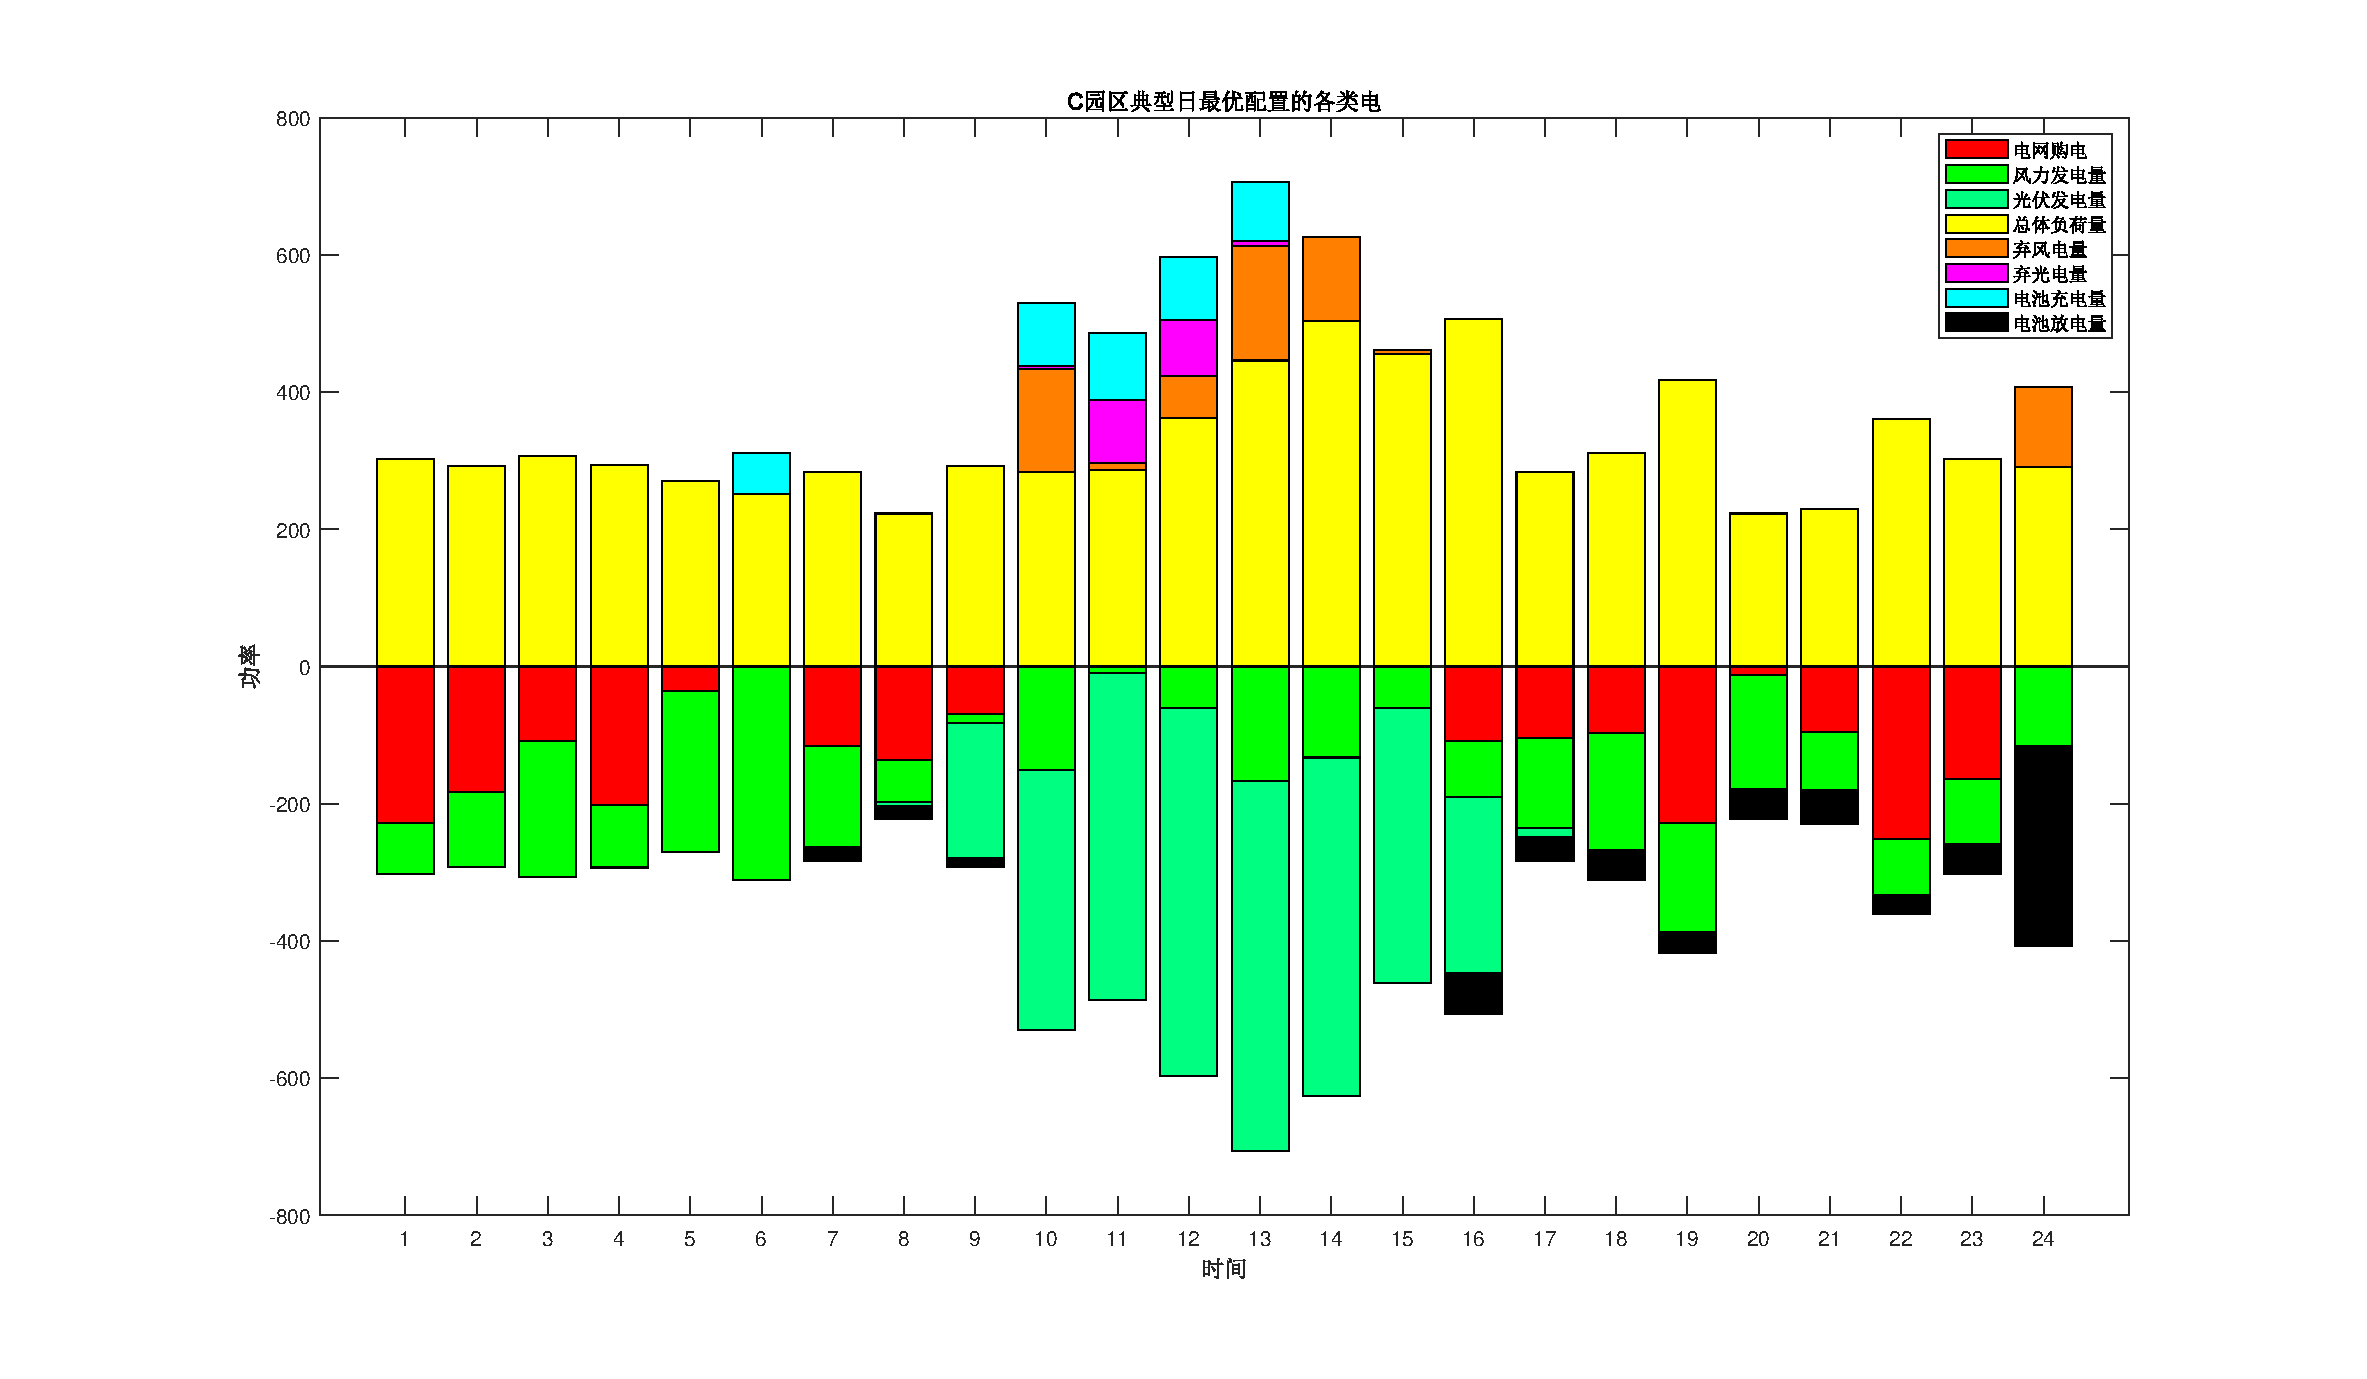
\includegraphics[width=.9\linewidth]{figures/Q1_3_C_sort.eps}  
  \subcaption{C园区的电量供需对比图}  
\end{minipage}  
\caption{C园区}  
\end{figure}

\begin{table}[!h]  
\centering  
\begin{tabular}{|l|l|l|l|}  
\hline  
\text{配置方案 } & \text{最优的最大充放电功率} \text{ (kW) } & \text{最优的最大容量} \text{ (kWh) } & \text{最小的总供电成本} \text{ (元) } \\  
\hline  
\text{A园区 }  & 275 & 413 & 5899.02 \\  
\hline  
\text{B园区  }  & 324  & 486 & 4744.11 \\  
\hline  
\text{C园区  }  & 291 & 437 & 4801.07 \\  
\hline  
\end{tabular}  
\caption{园区最优的储能功率、容量配置方案}  
\label{tab:curvature_values}  
\end{table} 

\newpage

\subsubsection{经济性对比分析} 

通过对比不同园区的总供电成本可以看出,各个园区在最优储能下总供电成本最小。 一方面,储能容量越大,可以吸收更多的风光富余电力,提高可再生能源利用率;同时,也能够更灵活地优化电力的时间分配,削峰填谷,降低购电成本。另一方面,储能设备的投资和运维成本也会随着容量的增大而提高。通过模拟退火算法可以求出综合考虑电池功率、储能和投资成本的最优储能配置。

\begin{figure}[!h]
\centering
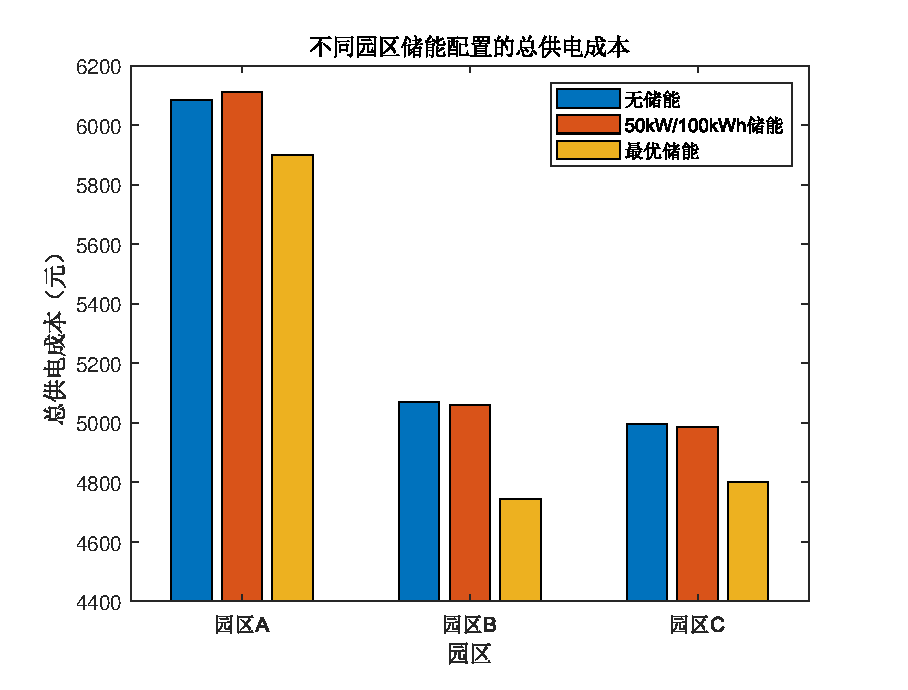
\includegraphics[width=.8\textwidth]{figures/1_3_对比.eps}
\caption{园区配置前后总供电成本对比示意图}
\end{figure}

\begin{table}[!h]  
\centering  
\begin{tabular}{|l|l|l|l|}  
\hline  
\text{不同配置方案的总供电成本} & \text{无储能} \text{ (元) } & \text{50kw/100kwh储能} \text{ (元) } & \text{最优储能} \text{ (元) } \\  
\hline  
\text{A园区 }  & 6084.88 & 6112.33 & 5899.02 \\  
\hline  
\text{B园区  }  & 5071.15 & 5058.77  & 4744.11 \\  
\hline  
\text{C园区  }  & 4996.48 & 4987.23 & 4801.07 \\  
\hline  
\end{tabular}  
\caption{园区最优的储能功率、容量配置方案}  
\label{tab:curvature_values}  
\end{table} 



\newpage 
  
 \subsection{问题二模型的建立与求解}
\subsubsection{未配置储能经济性分析}
根据题目所给数据,将ABC园区各个时段的风电、光伏发电量、负荷功率相加,得到联合园区的供电和用电信息,从而绘出联合园区园区各个时刻对应的总产电量、负荷电量、向主电网购电量、弃风弃光电量曲线,可以看出联合园区园区在9时至13时期间发电量大于负荷电量,存在明显的弃电损失。

\begin{figure}[!h]
\centering
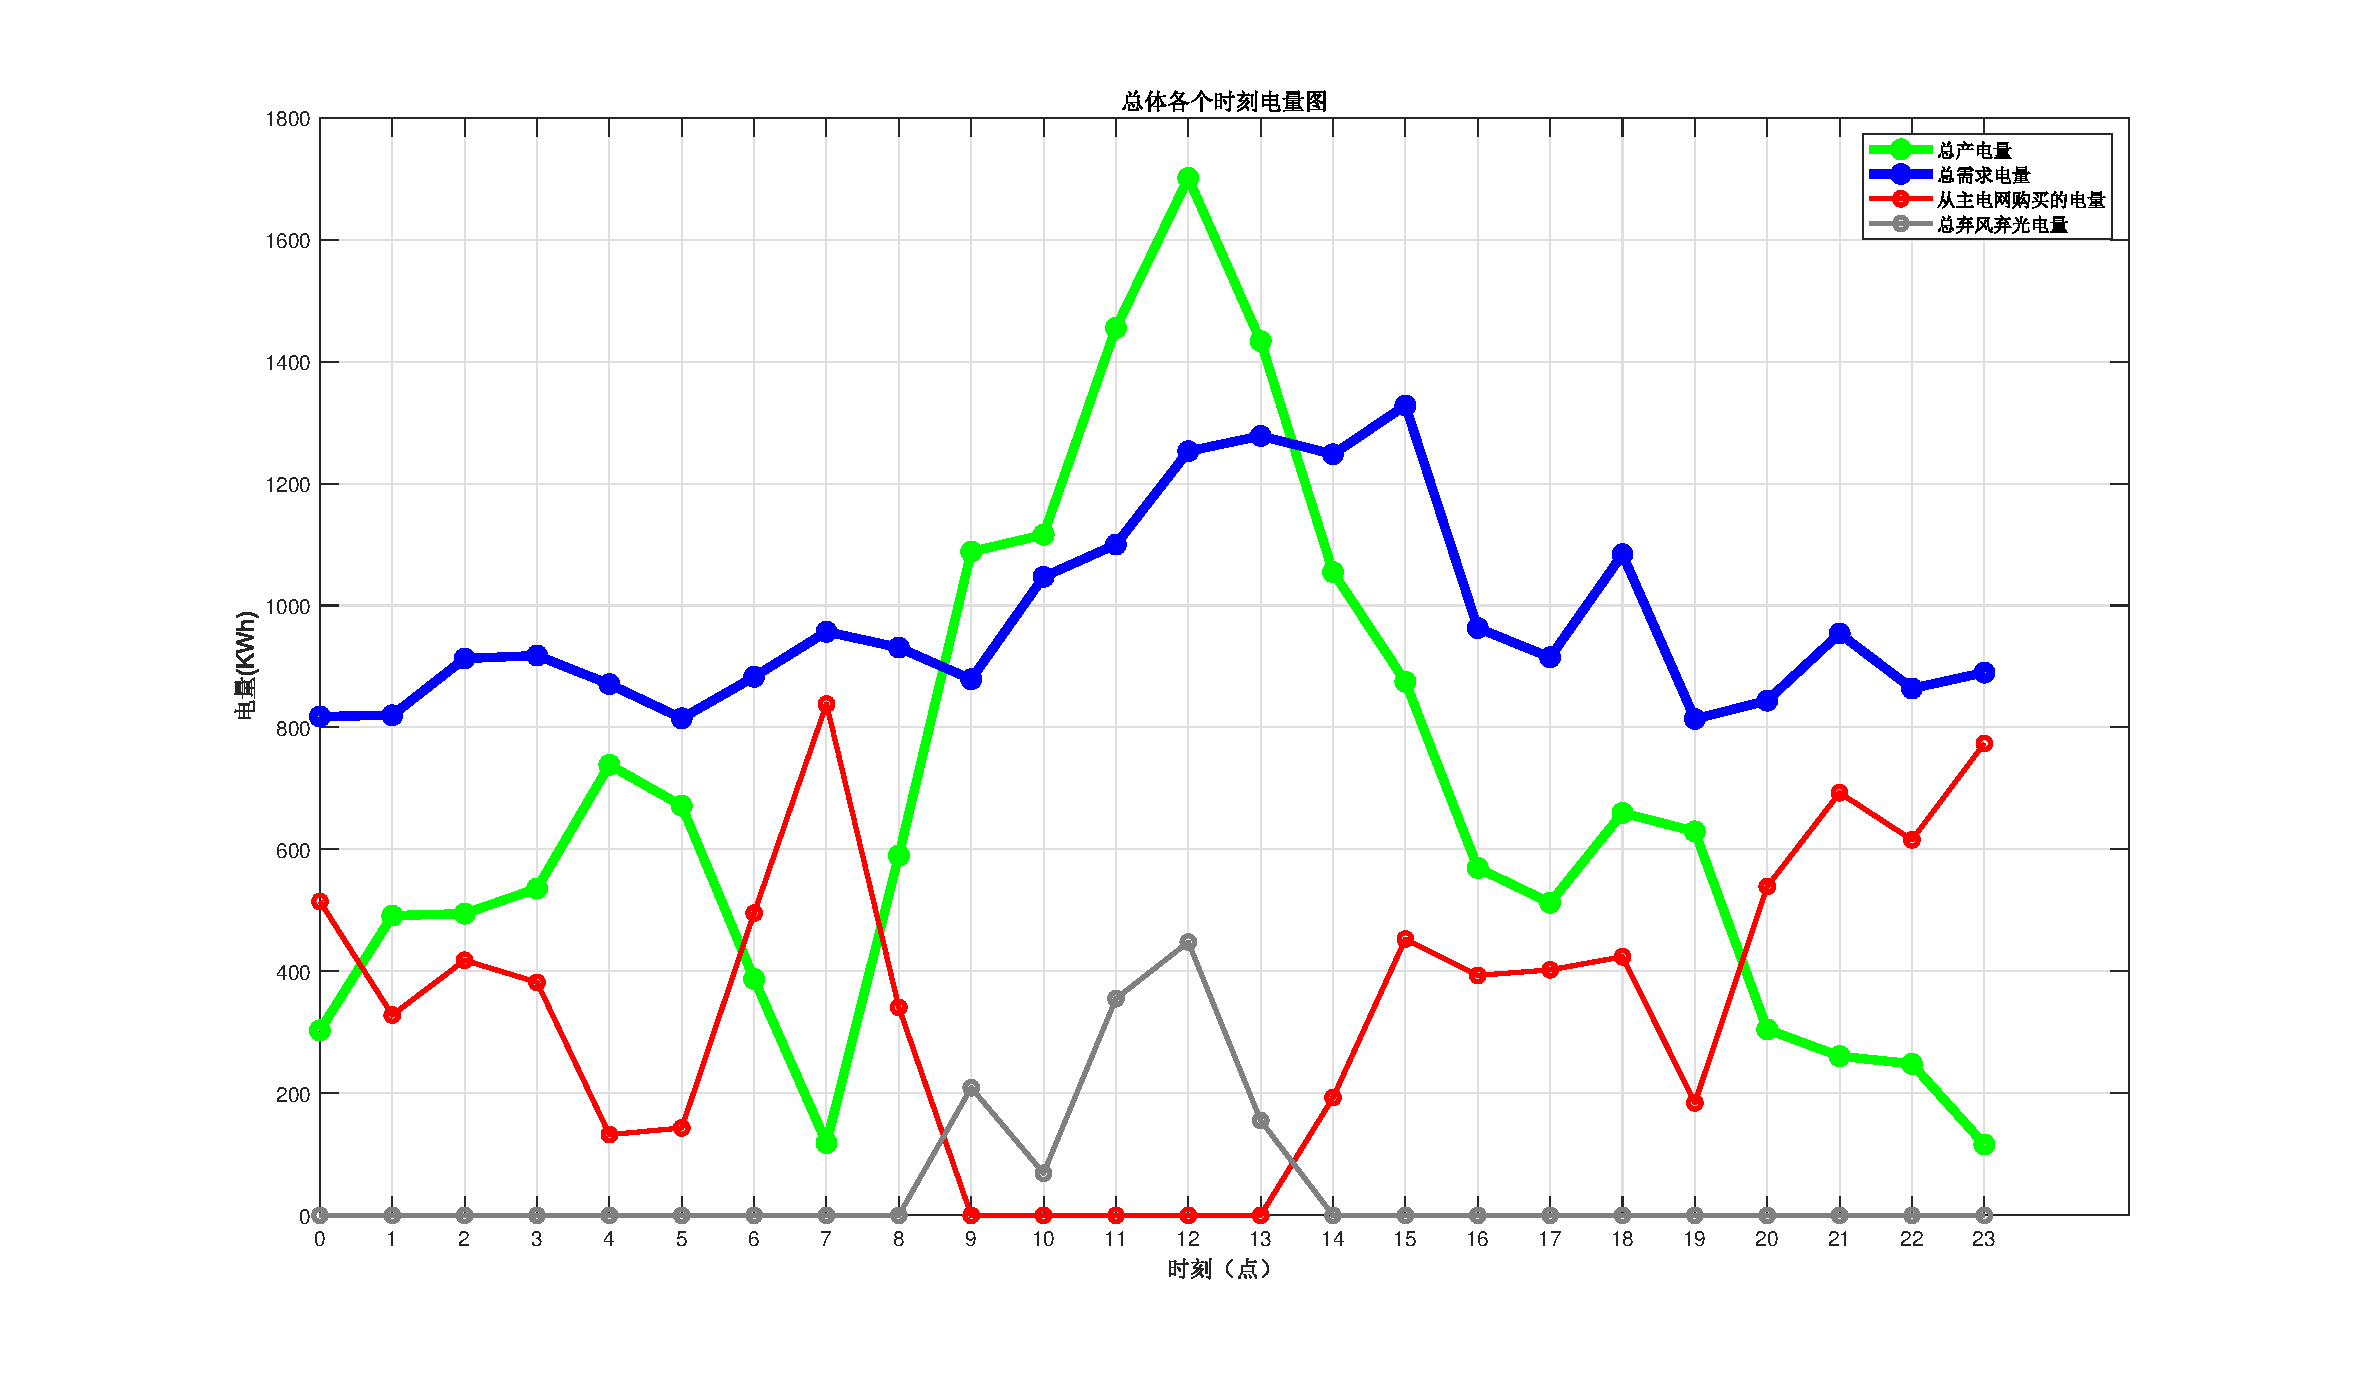
\includegraphics[width=.6\textwidth]{figures/Q2line.eps}
\caption{联合园区供需对比示意图}
\end{figure}

风光发电功率:
\begin{equation}
\left\{\begin{array}{l}
P_w(t)=\left[P_{w p u 1}(t)+P_{w p u_2}(t)+P_{w p u 3}(t)\right] \times P_w \\
P_s(t)=\left[P_{s p u 2}(t)+P_{s p u 2}(t)+P_{s p u 3}(t)\right] \times P_{p v}
\end{array}\right.
\end{equation}

日负荷功率:
\begin{equation}
L(t)=L_A(t)+L_B(t)+L_C(t)
\end{equation}

\textbf{总购电量:}

\begin{equation}
\begin{aligned}
E_{\text {sum }} & =\sum_{t=1}^{24} L(t) \\
& =\sum_{t=1}^{24}\left(L_A(t)+L_B(t)+L_C(t)\right)
\end{aligned}
\end{equation}

\textbf{其它经济要素:}

由问题一中的(6)式、(7)式、(8)式可得联合园区的总弃风弃光电量、总供电成本和单位电量平均供电成本:
\begin{equation}
\left\{\begin{array}{l}
E_{\text {discard }}=\sum_{t=1}^{24} \max \left\{0, P_{\text {sum }}(t)-L(t)\right\} \\
C_{\text {total }}=\sum_{t=1}^{24}\left(P_{w l}(t) w_f+P_{s l}(t) w_s\right)+E_{\text {grid }} \times w_g \\
C_{\text {avg }}=\frac{C_{\text {total }}}{\sum_{t=1}^{24} L(t)}
\end{array}\right.
\end{equation}

\textbf{结果:}

\begin{table}[!h]  
\centering  
\begin{tabular}{|l|l|l|l|l|}  
\hline  
\text{经济要素 }  & \text{总购电量} & \text{弃风弃光电量} & \text{总供电成本} & \text{单位电量平均供电成本} \\  
\hline  
\text{联合园区 }  & 23387.00 & 1237.17 & 15107.66 & 0.65  \\  
\hline   
\end{tabular}  
\caption{不同园区的经济要素}  
\label{tab:curvature_values}  
\end{table} 


\textbf{影响其经济性的关键因素分析:}

  \begin{figure}[!h]  
\centering 
\begin{minipage}{.5\textwidth}  
  \centering  
  \includegraphics[width=.9\linewidth]{figures/2_1_饼图2.pdf}  
  \subcaption{联合园区各类电量占比示意图}  
\end{minipage}%  
\begin{minipage}{.5\textwidth}  
  \centering  
  \includegraphics[width=.9\linewidth]{figures/2_1_饼图.pdf}  
  \subcaption{联合园区各类成本占比示意图}  
\end{minipage}  
\caption{联合园区的经济要素对比图}  
\end{figure} 


从表格数据和各个园区的成本饼状图可以看出,联合园区中,有效风光发电量占各类电量的$60\%$以上,联合园区实现了较好的电量自给,向主电网的购电量占比相较于独立园区运营明显减少;但是,从各类电费占比图中,可以看出向主电网的购电成本占园区电费成本的$50 \%$以上,风力、光优购电成本在不同园区的花费占比可达到 $40 \% \sim 50 \%$,说明向主电网的购电成本为园区购电成本的的主要因素。结合实际情况,风光发电具有间歇性和波动性的特点,其出力与园区的电力负荷需求往往存在时序上的不匹配,与所求结果相符。

 
  \subsubsection{联合园区储能配置模型}\label{ll}
  
相较于问题一的模型,问题二考虑联合园区的作用,将各园区的风光发电量和负荷相加,允许弃光弃风,仍以总供电成本最小为目标,对联合园区微电网风光储协调配置调度进行优化。

\textbf{目标函数:}

总供电成本:
\begin{equation}
C_{\text {total }}=\sum_{t=1}^{24}\left(E_{\text {grid }}(t) \cdot w_g+P_{w 0}(t) w_f+P_{s 0}(t) w_s\right)+C_{\text {day }}
\end{equation}
  
  
  \subsubsection{SQP算法求解}\label{lll}
在上述模型中,目标函数为系统总成本,包括电网购电成本、弃电成本和储能系统的固定成本。约束条件包括能源平衡、弃风电量和弃光电量不大于相应的发电量、充放电功率不超过最大功率、储能SOC约束。

我们利用SQP算法通过逐步逼近原始非线性优化问题,解决储能系统的最优调度问题。SQP算法通过将原始的非线性问题分解为一系列的二次规划问题(QP)来逐步逼近最优解。每一步迭代中,算法解决一个近似的二次规划问题,在实际应用中,我们通过使用$MATLAB$里的$fmincon$函数进行SQP优化求解。

具体步骤如下:


\begin{figure}[H]  
	\centering
	
	\scriptsize  
	
	%像素点,用于连接转移线
	\begin{tikzpicture}[node distance=2cm]
		%定义流程图具体形状
		\node (start1) [startstop] {定义初始值和边界条件};
		\node (in1) [process, below of=start1] {定义约束函数、目标函数};
		\node (pro1) [process, below of=in1,] {使用 fmincon 函数调用SQP算法进行优化求解};
		\node (stop1) [startstop, below of=pro1]{解析优化结果};
		
		%连接具体形状
		\draw [arrow](start1) -- (in1);
		\draw [arrow](in1) --  (pro1);
		\draw [arrow](pro1) --  (stop1);
	\end{tikzpicture}
	\caption{第三题求解流程}
	\label{dthz}
\end{figure} 

  \begin{figure}[!h]  
\centering 
\begin{minipage}{.45\textwidth}  
  \centering  
  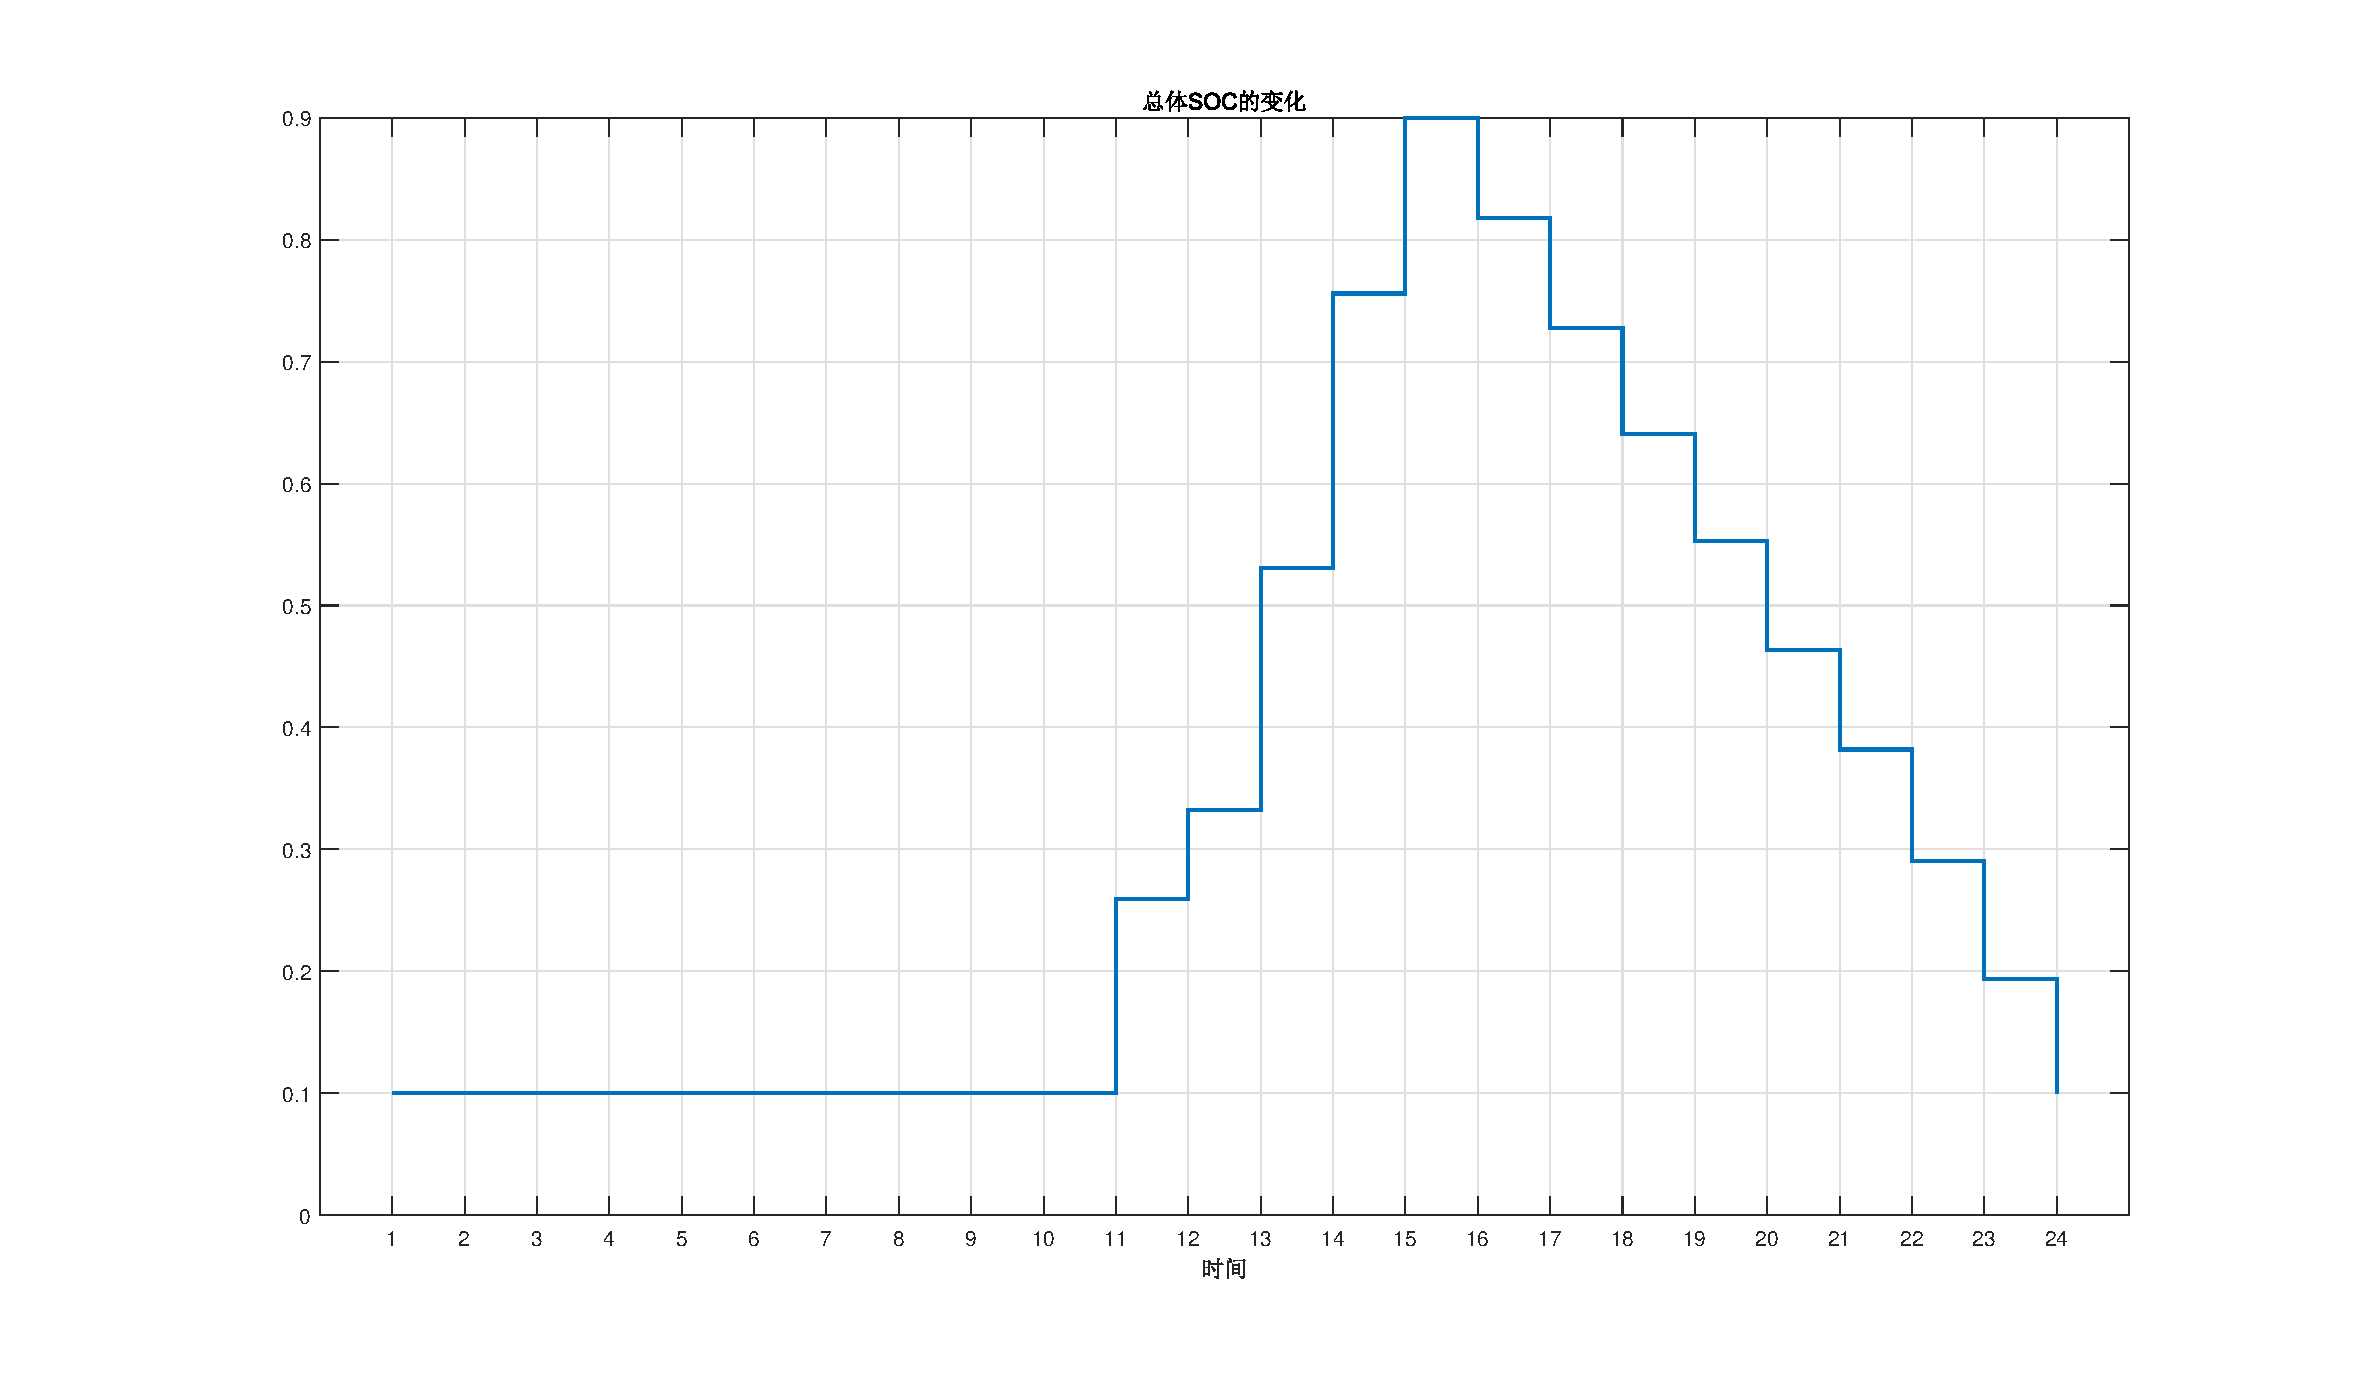
\includegraphics[width=.9\linewidth]{figures/2_2_SOC.eps}  
  \subcaption{SOC变化示意图}  
\end{minipage}  
\begin{minipage}{.45\textwidth}  
  \centering  
  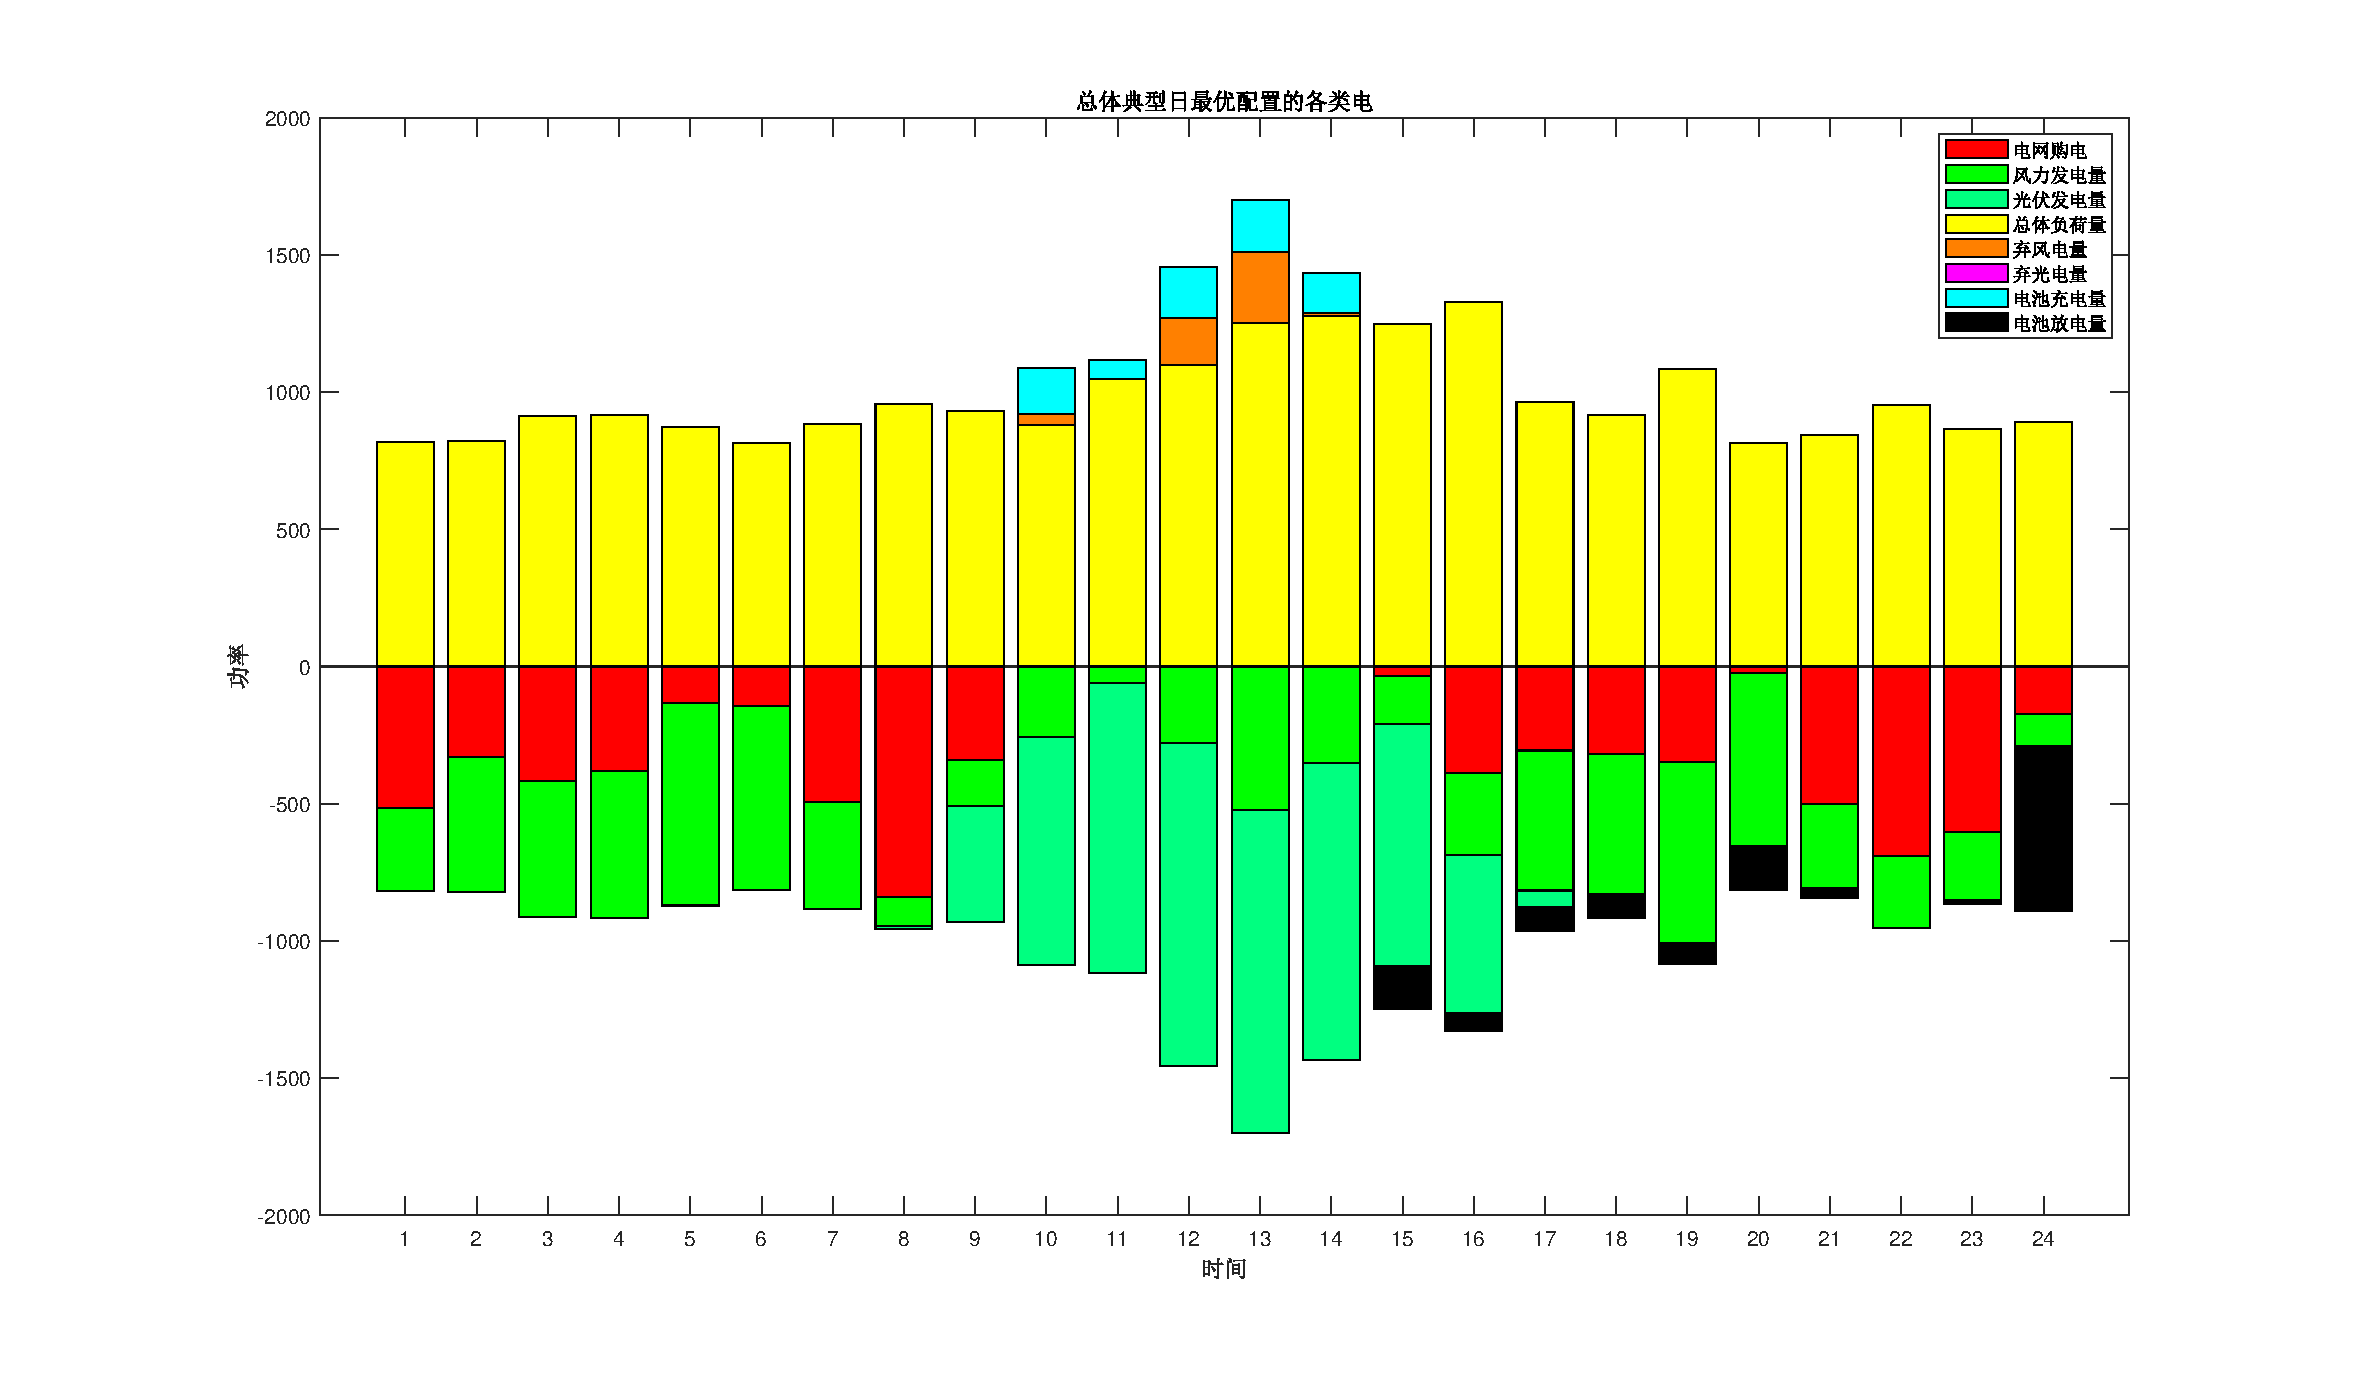
\includegraphics[width=.9\linewidth]{figures/2_2_sort.eps}  
  \subcaption{各类用电量变化示意图}  
\end{minipage}  
\caption{联合园区的储能配置示意图}  
\end{figure} 


  
\begin{table}[!h]  
\centering  
\begin{tabular}{|l|l|l|l|}  
\hline  
\text{储能配置方案} & \text{最大充放电功率} \text{kW } & \text{最大储能容量} \text{kWh } & \text{总供电成本} \text{ (元) } \\  
\hline  
\text{联合园区 }  & 600 & 900 & 14769 \\  
\hline    
\end{tabular}  
\caption{园区最优的储能功率、容量配置方案}  
\label{tab:curvature_values}  
\end{table} 
  
\subsubsection{联合园区经济性收益的分析}

\begin{table}[!h]  
\centering  
\begin{tabular}{|l|l|l|l|l|}  
\hline  
\text{经济要素 }  & \text{总购电量} & \text{弃风弃光电量} & \text{总供电成本} & \text{单位电量平均供电成本} \\  
\hline  
\text{联合园区 }  & 23387.00 & 1237.17 & 15107.66 & 0.65  \\  
\hline   
\text{三个独立园区之和 }  & 23387.00 & 2976.72 & 16119.34 & 0.69  \\  
\hline   
\end{tabular}  
\caption{不同园区的经济要素}  
\label{tab:curvature_values}  
\end{table} 

通过表格6,可以明显看出未配置储能时联合园的总购电量、弃风弃光电量、总供电成本都有明显的下降,原因是通过园区联合运营,可以实现风光发电互补,减小对主电网的依赖,从而减少向主电网的购买量,降低供电成本。 

针对风电价格、光伏发电价格、主电站价格进行灵敏度分析, 分别控制一个变量变化,其他变量与题目条件一致,探究不同价格对园区运行经济性影响,拟合结果如下:
  \begin{figure}[!h]  
\centering  
\begin{minipage}{.5\textwidth}  
  \centering  
  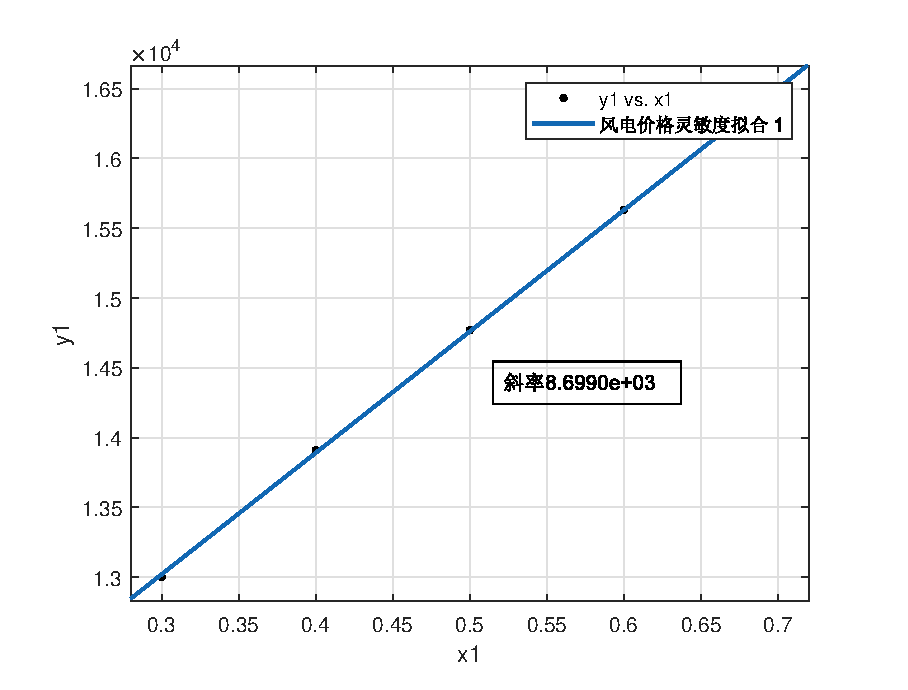
\includegraphics[width=.8\linewidth]{figures/2_3风.eps}  
  \subcaption{风电价格灵敏度分析}  
\end{minipage}%  
\begin{minipage}{.5\textwidth}  
  \centering  
  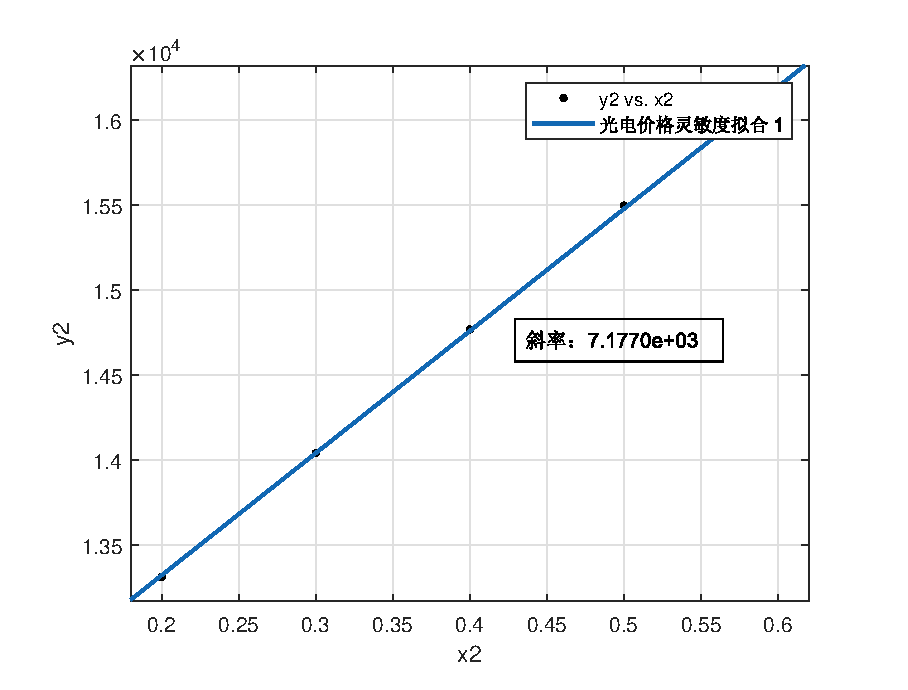
\includegraphics[width=.8\linewidth]{figures/2_3光.eps}  
  \subcaption{光电价格灵敏度分析}  
\end{minipage}  
\begin{minipage}{.5\textwidth}  
  \centering  
  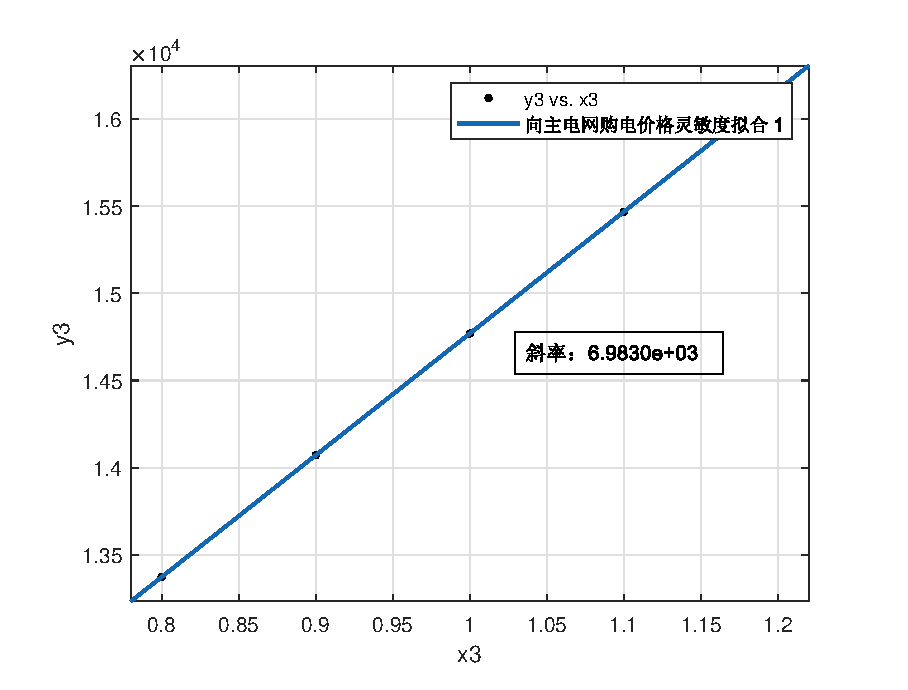
\includegraphics[width=.8\linewidth]{figures/2_3电网.eps}  
  \subcaption{主电站价格灵敏度分析}  
\end{minipage}  
\caption{各类发电灵敏度分析}  
\end{figure} 
\newpage

对比三个斜率:8699(风电)> 7177(光电)> 6983(主电网),结合上面三个图可以看出, 联合园区对风电发电价格更敏感。可以得到推论:风电价格对园区运行经济性的影响最大,为关键因素。

  
\subsection{问题三模型}


  \subsubsection{风光储协调配置模型}\label{ll}
第三问在第二问的基础上新增加了风电、光伏的配置条件情况,需要我们综合考虑风、光、储系统的配置成本、购电策略、充放电策略,求出成本最低的配置方案。由于风电和光电受环境影响大,而A、B、C园区之间的位置关系位置,故B、C的风电对A参考价值低,A、C的光电对B的参考价值低,故认为A不可新增风电设备,B不可新增光电设备,否则会引起较大的误差。

第一阶段:风、光、储系统的配置策略

基于第一、二问,除定义储能系统的功率变量$P_{m a x}$变量 $E_{m a x}$,还新定义了风光配置变量,用来描述风、光、储系统的配置策略:

园区的新增风电电源的功率 $\Delta P_w$

园区的新增光伏电源的功率 $\Delta P_s$

则:
\begin{equation}
\left\{\begin{array}{l}
P_{w, \text { new }}=\Delta P_w \times P_{\text {wpu }} \\
P_{\text {s, new }}=\Delta P_s \times P_{\text {spu }} \\
P_{\text {sum, new }}=P_{w, \text { new }}+P_{\text {s, new }}
\end{array}\right.
\end{equation}

变量 $E_{n \times x}$, 还新定义了风光配置变量, 用来描述冈、光、储系统的配置策略
  
  
\textbf{目标函数:}
  
\begin{equation}
C_{\text {total }}=\sum_{t=1}^{24}\left(E_{\text {grid }}(t) \cdot w_g+P_{w 0}(t) w_f+P_{s 0}(t) w_s\right)+C_{\text {cost }}
\end{equation}

其中:

$$
C_{\text {cost }}=\frac{\Delta P_w \times 3000+\Delta P_s \times 2500+P_{\text {max }} \times 800+E_{\text {max }} \times 1800}{5 \times 365}
$$

$$
P_{w 0}=\max \left\{P_w(t)-E_{\text {discard }}(t), 0\right\}
$$

$$
P_{s 0}= \begin{cases}\max \left\{P_s(t)+P_w(t)-E_{\text {discard }}(t), 0\right\}, & P_{w 0}=0 \\ \max \left\{P_s(t)-E_{\text {discard }}(t), 0\right\}, & P_{w 0} \neq 0\end{cases}
$$

\textbf{约束条件:}

向主电网的购电量约束:如果储能系统放电不足,则购电补充:
\begin{equation}
\left.E_{\text {grid }}(t)=\max \left\{L(t)-P_{\text {sum }}(t)-P_{\text {sum,new}}(t)-P_{\text {discharge }}(t), 0\right)\right\}
\end{equation}

弃风弃光电量约束:如果储能系统充电已达上限,则弃风弃光:
\begin{equation}
\left.E_{\text {discard }}(t)=\max \left\{P_{\text {sum }}(t)+P_{\text {sum,new }}(t)-L(t)-P_{\text {charge }}(t), 0\right)\right\}
\end{equation}

投资回报约束:
\begin{equation}
\begin{aligned}
& \sum_{i=1}^{24} E_{\text {grid }}(i) \times w_g +\sum_{i=1}^{24}\left[P_w(i)-E_{\text {discard }}(i)-P_{w, \text { new }}(t)\right] \times w_f \\
&+\sum_{i=1}^{24}\left[P_s(i)-E_{\text {discard }}(i)-P_{s, \text { new }}(t)\right] \times w_s \\
&+\left[\Delta P_w \times 3000+\Delta P_s \times 2500+P_{\text {max }} \times 800+E_{\text {max }} \times 1800\right] / (365 \times 5)< C
\end{aligned}
\end{equation}

其中,$C$为未配置情况下的,一天的电力花费。

充放电状态约束:
\begin{equation}
P_{\text {discharge }}(t) P_{charge}(t)=0
\end{equation}

根据充放电机制,可以列出SOC变化公式:
$$
\operatorname{SOC}(t+1)=\operatorname{SOC}(t)+\frac{\eta \cdot P_{\text {charge }}-P_{\text {charge }}(t) / \eta}{E_{\max }}
$$

其他条件约束:
\begin{equation}
\left\{\begin{array}{l}
\mathrm{SOC}_{\text {min }} \leqslant \mathrm{SOC}(t) \leqslant S O C_{\text {max }} \\
\mathrm{SOC}(0)=\mathrm{SOC}(23)\\
0 \leqslant P_{\text {charge }}, P_{\text {discharge }} \leqslant P_{\text {max }} \\
E_{\text {grid }} \geqslant 0 \\
L(t)=P_{\text {gen }}(t)+P_{\text {gen,new }}(t)+P_{\text {discharge }}(t)-P_{\text {charge }}(t)+E_{\text {grid }}(t)
\end{array}\right.
\end{equation}
  
\textbf{模型的求解}

基于第一、二问的SQP算法,求出结果如下:


  \begin{figure}[!h]  
\centering 
\begin{minipage}{.5\textwidth}  
  \centering  
  \includegraphics[width=.99\linewidth]{figures/Q31_A_SOC.eps}  
  \subcaption{A园区SOC状态示意图}  
\end{minipage}%  
\begin{minipage}{.5\textwidth}  
  \centering  
  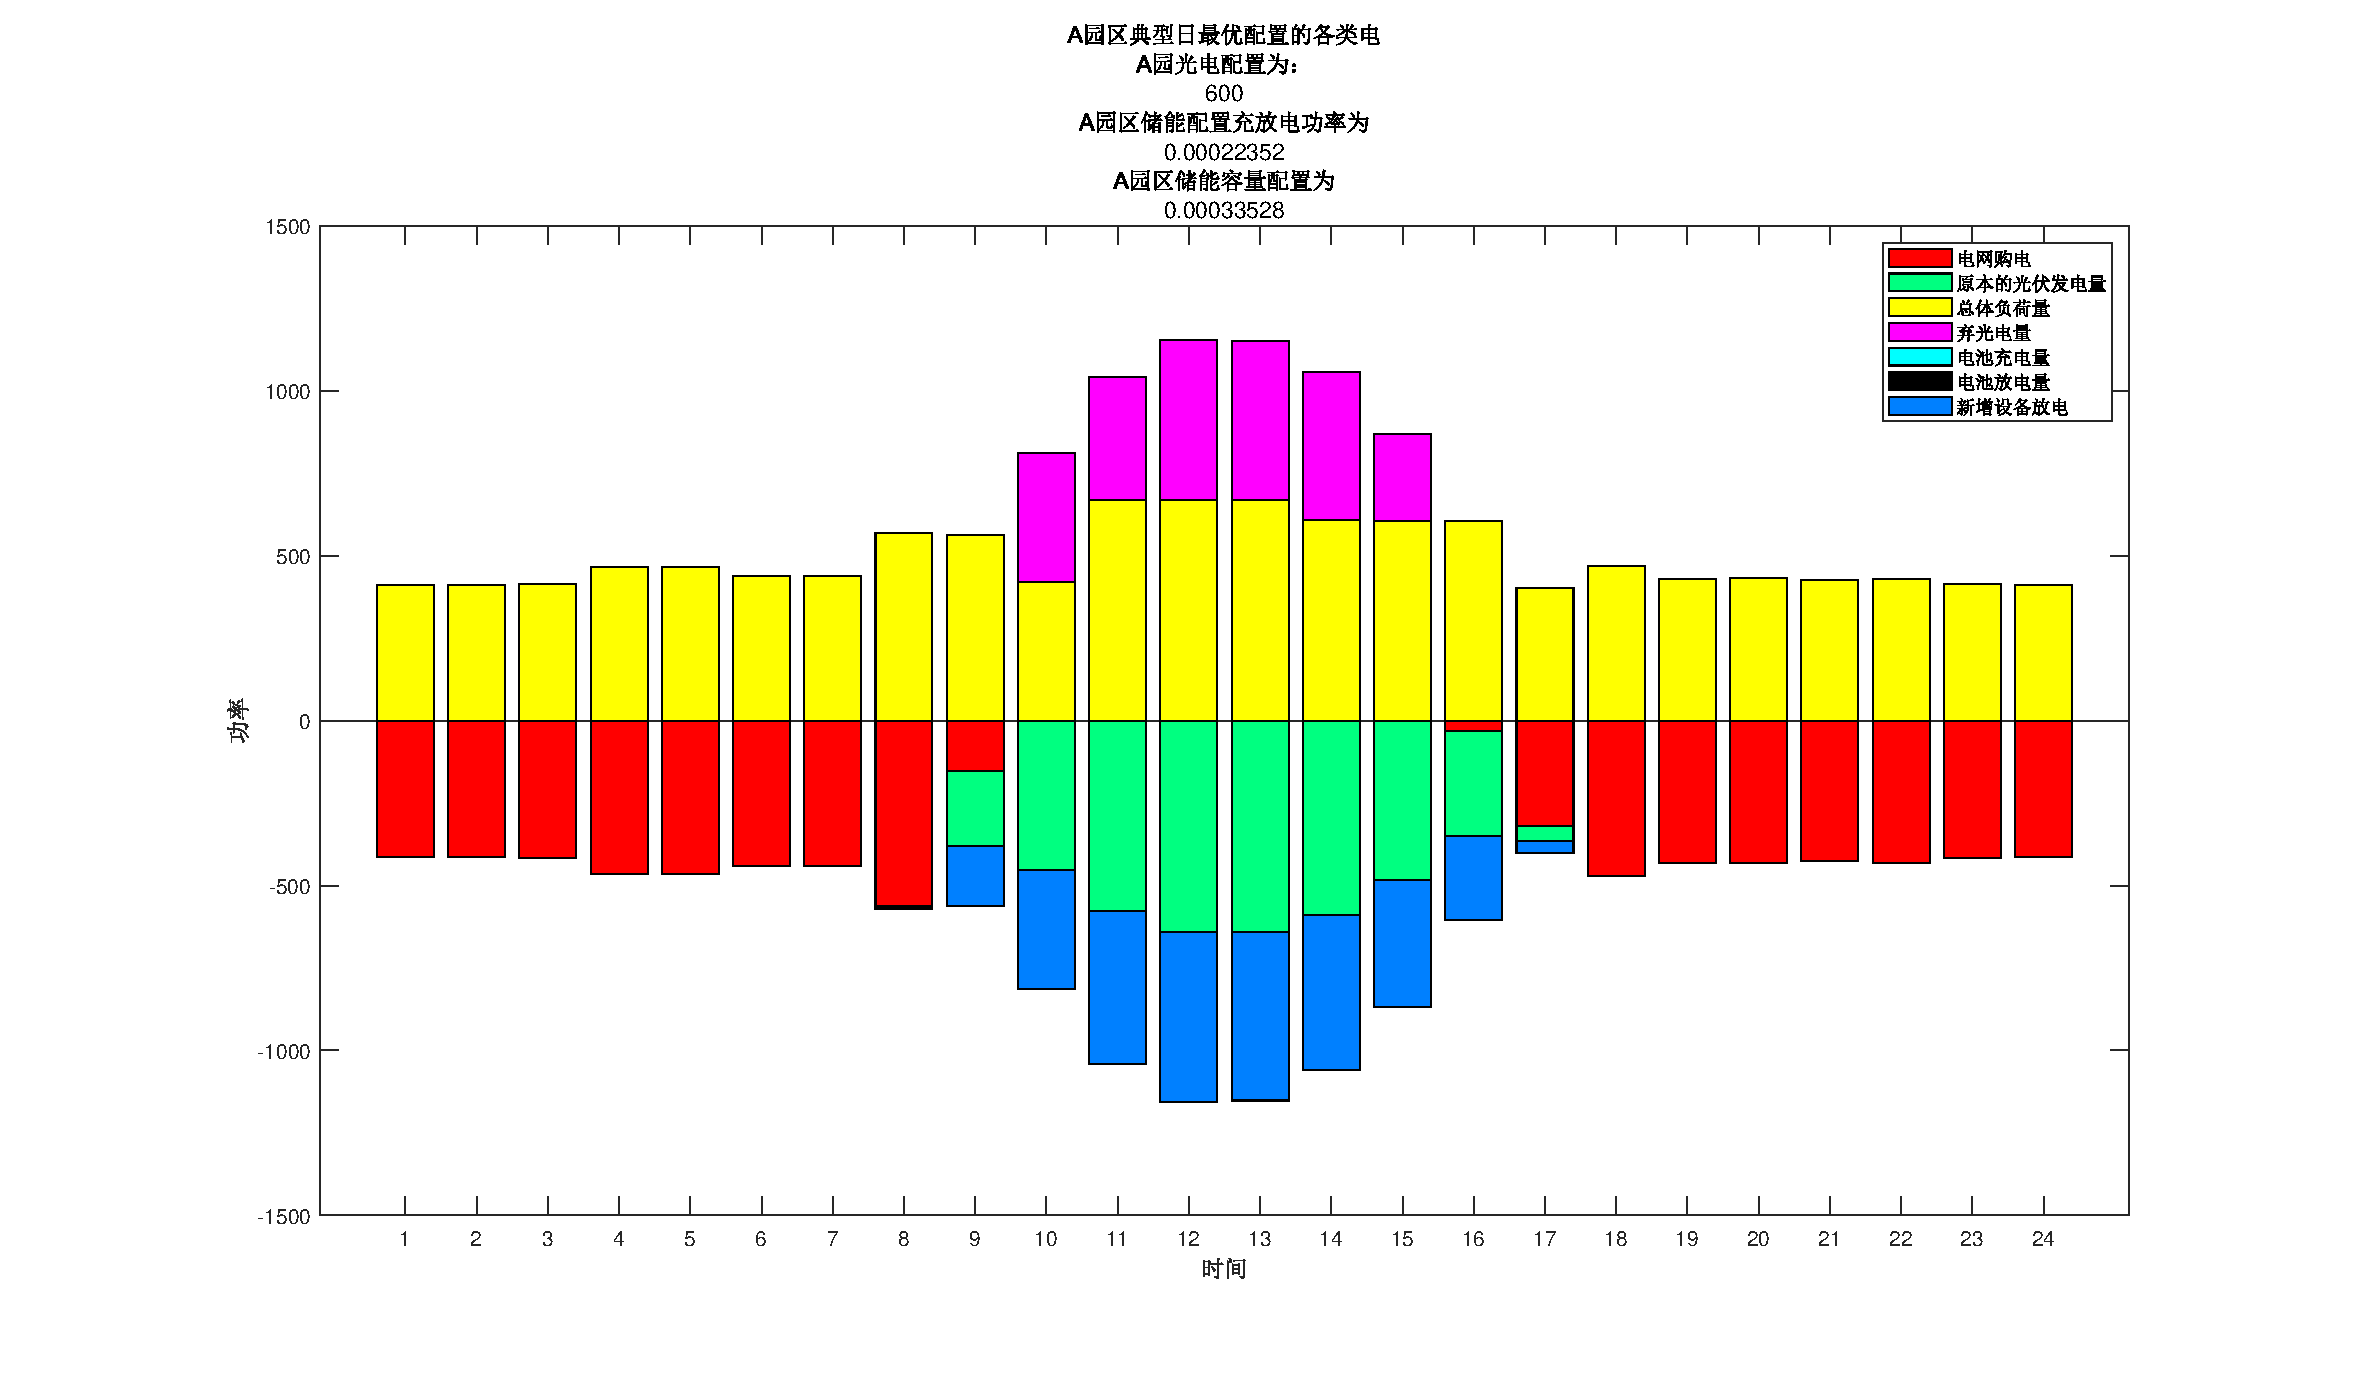
\includegraphics[width=.99\linewidth]{figures/Q31_A.eps}  
  \subcaption{A园区电网状态示意图}  
\end{minipage}  
\caption{A园区}  
\end{figure} 
     \begin{figure}[!h]  
\centering 
\begin{minipage}{.5\textwidth}  
  \centering  
  \includegraphics[width=.99\linewidth]{figures/Q31_B_SOC.eps}  
  \subcaption{B园区SOC状态示意图}  
\end{minipage}%  
\begin{minipage}{.5\textwidth}  
  \centering  
  \includegraphics[width=.99\linewidth]{figures/Q31_B.eps}  
  \subcaption{B园区电网状态示意图}  
\end{minipage}  
\caption{B园区}  
\end{figure} 
 \begin{figure}[!h]  
\centering 
\begin{minipage}{.5\textwidth}  
  \centering  
  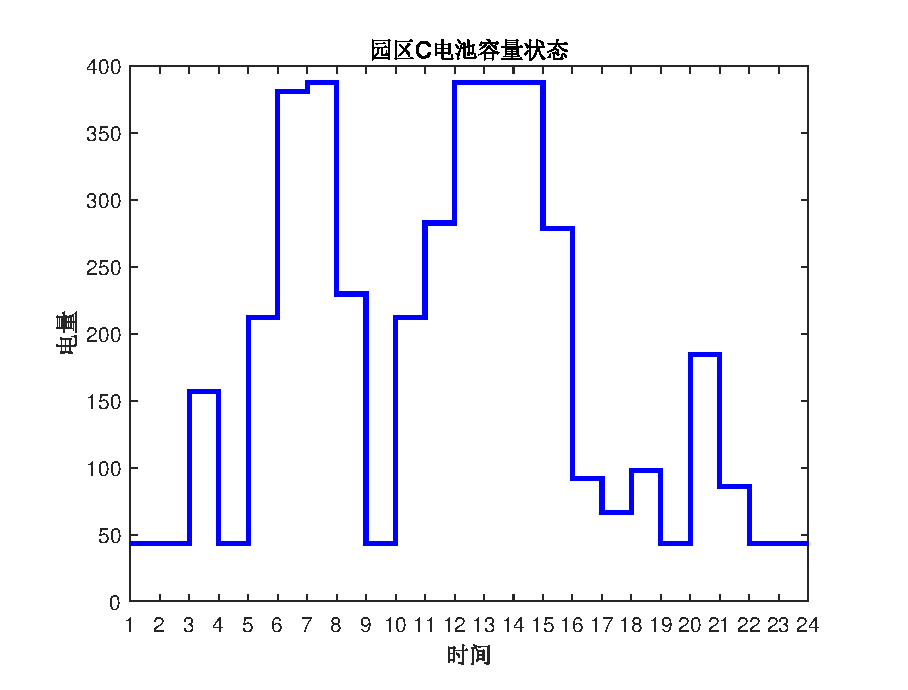
\includegraphics[width=.99\linewidth]{figures/31C电池.eps}  
  \subcaption{C园区SOC状态示意图}  
\end{minipage}%  
\begin{minipage}{.5\textwidth}  
  \centering  
  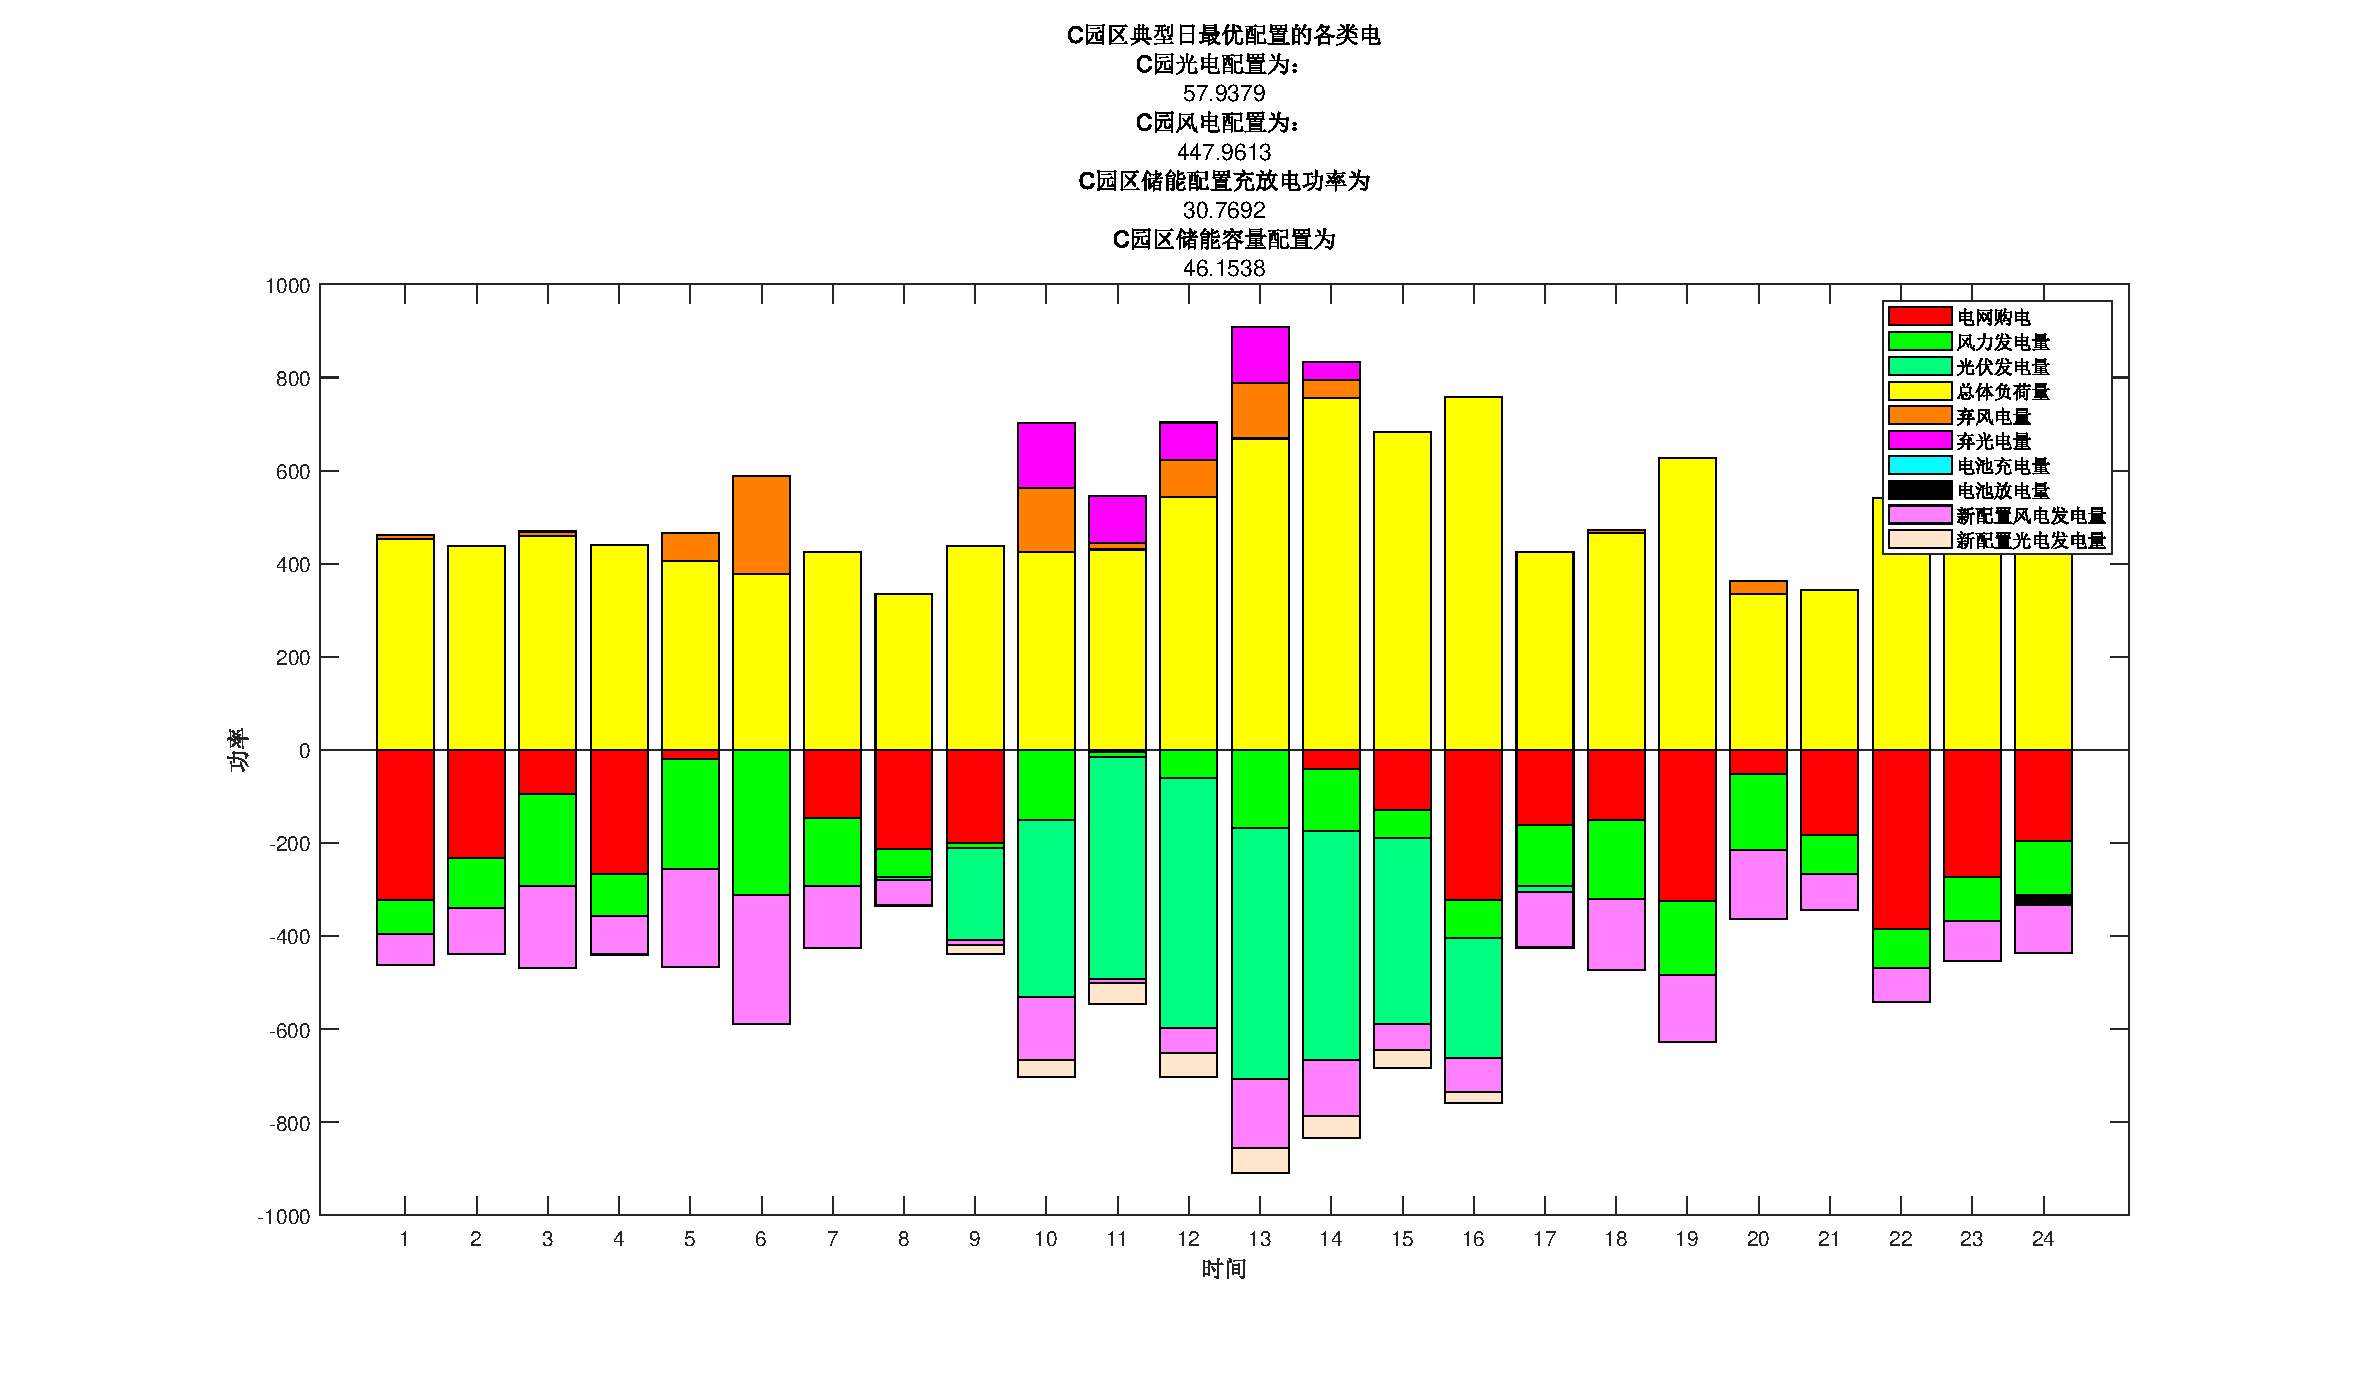
\includegraphics[width=.99\linewidth]{figures/Q31_Csort.eps}  
  \subcaption{C园区电网状态示意图}  
\end{minipage}  
\caption{C园区}  
\end{figure} 
 \begin{figure}[!h]  
\centering 
\begin{minipage}{.5\textwidth}  
  \centering  
  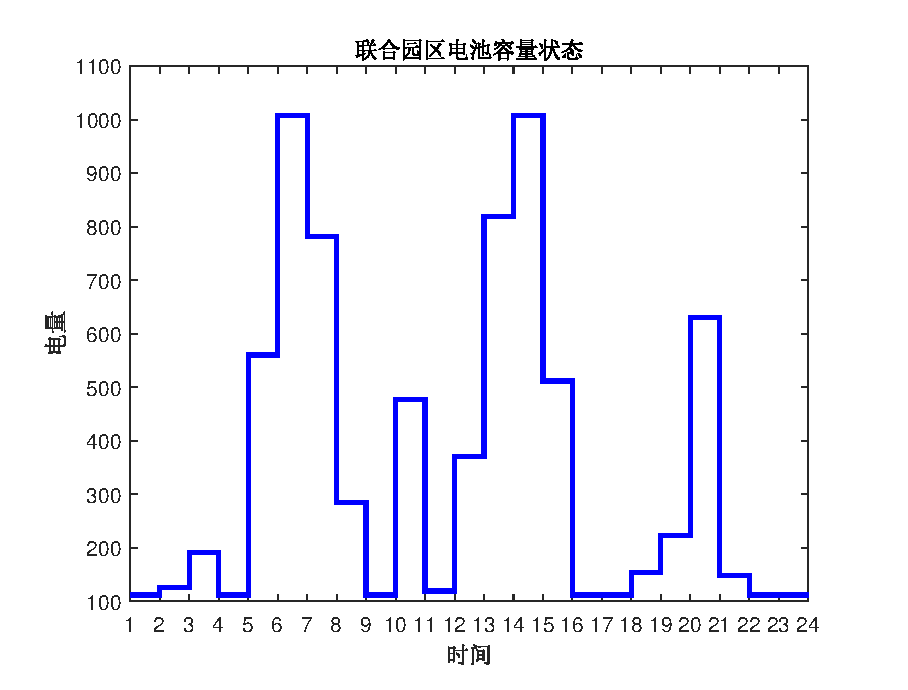
\includegraphics[width=.9\linewidth]{figures/31联合园区电池.eps}  
  \subcaption{联合园区SOC状态示意图}  
\end{minipage}%  
\begin{minipage}{.5\textwidth}  
  \centering  
  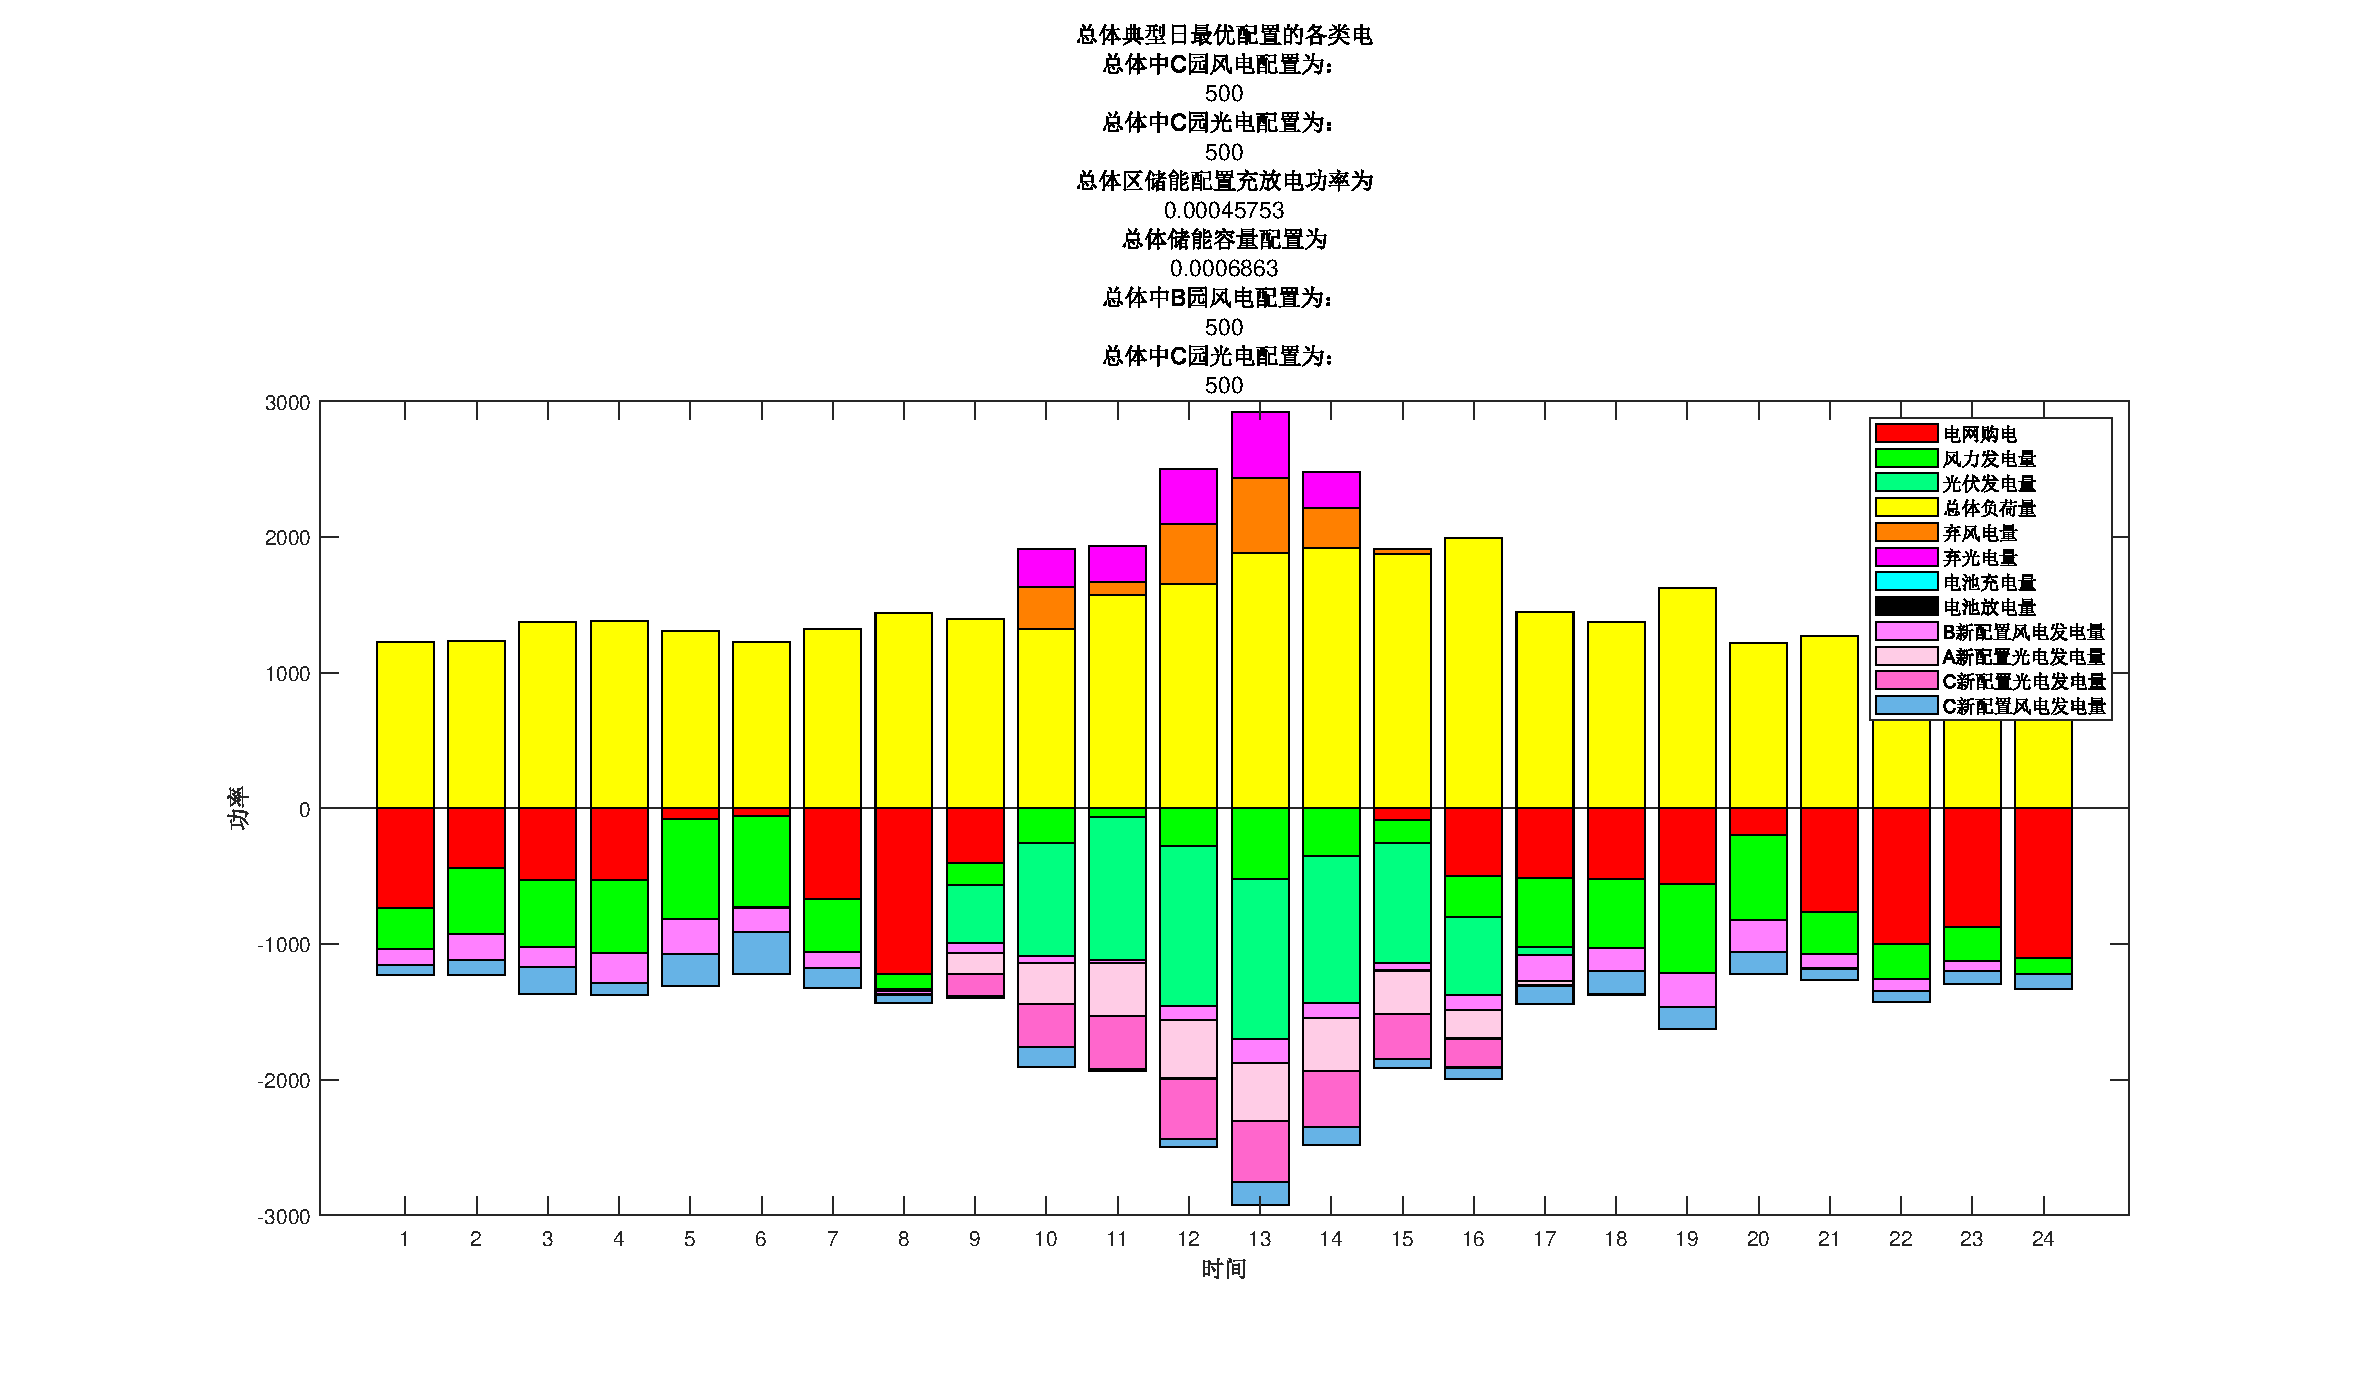
\includegraphics[width=.9\linewidth]{figures/Q31_Usort.eps}  
  \subcaption{联合园区电网状态示意图}  
\end{minipage}  
\caption{联合园区}  
\end{figure} 
\newpage
  

  \subsubsection{全年协调配置方案模型}\label{ll}
  
  基于上一问的模型,结合全年$12$个月的典型日风光发电功率数据和分时电价策略, 制定购电计划和储能运行策略。设$C_{\text {total }}(i)$ 为第 $i$ 个月的最小日成本,$Month(i)$为第 $\mathrm{i}$ 个月对应天数。则目标函数为年最低成本:
  \begin{equation}
C_{\text {year }}=\sum_{i=1}^{12} C_{\text {total }}(i) \cdot Month_(i)
\end{equation}

其中
$$
W_g= \begin{cases}1 & 7 \leqslant t<22 \\ 0.4 & 0 \leqslant t<7 \text { 或 } 22<t \leqslant 24\end{cases}
$$

投资回报约束:

设 $C_{\text {new }}$ 为配罢后一年的发电总成本,$C_0$为无配置的一年的发电总成本,
$$
C_0-C_{\text {new }}>\frac{\Delta P_w \times 3000+\Delta P_s \times 2500+P_{\text {max }} \times 800+E_{\text {max }} \times 1800}{5}
$$


\textbf{运行结果}
\begin{table}[!h]    
\centering    
\small % 减小字体大小  
\begin{tabular}{|c|c|c|c|c|c|}  % 使用c来居中内容,并根据需要调整列宽  
\hline    
\text{配置方案} & \text{储能功率} \text{(kW)} & \text{储能容量} \text{(kWh)} & \text{新增风电功率} \text{(kW)} & \text{新增光电功率} \text{(kW)} & \text{供电成本} \text{(元)} \\    
\hline    
A园区  & 30.5372 & 113.1394 & 0 & 1789.8489 & 4165.18867 \\    
\hline    
B园区  & 150.2351 & 153.4111 & 1521.5117 & 0 & 3929.61333 \\    
\hline    
C园区  & 17.6068 & 35.134 & 1399.8653 & 1405.2845 & 4966.33793 \\    
\hline    
\end{tabular}    
\caption{园区最优的风、光、储配置方案}    
\label{tab:curvature_values}    
\end{table}


总供电成本为:13061.13333元。

\textbf{经济性分析}

对比新增风光电源前后经济要素显示,最优协调配置方案可显著降低园区能源成本。通过合理配置风、光、储能系统,实现了园区能源需求与供给的优化匹配,进而提高了能源利用效率。优化后的方案不仅有效控制了园区能源成本,还有助于降低对传统能源的依赖,提升园区的能源可持续性。这一方案将为园区的未来发展奠定坚实基础,为经济可行性与环境友好型能源管理提供了重要实践路径。

 
\section{模型的评价与推广}
\subsection{优点与缺点}
\subsubsection{优点}
1. 综合考虑多种因素:
    该模型综合考虑了光伏、风电发电量、电网购电量、弃电量、充放电等多种因素,能够较全面地反映实际能源系统的复杂性。

2. 优化函数:
    采用模拟退火算法和SQP算法进行非线性优化,能够处理复杂的约束条件和目标函数,找到全局最优解。

3. 储能系统建模:
    考虑了储能系统的充放电功率、容量、效率以及SOC变化,这对现代能源系统中的储能管理具有重要意义。


\subsubsection{缺点}
1. 数据依赖性强:
    模型依赖于具体的负荷和发电数据,若输入数据质量不高或不准确,优化结果可能不具参考价值。

2. 未考虑动态变化:
    本文提出得数学模型未考虑动态变化和不确定性。在实际应用中, 风光发电的输出功率会受到天气、季节等因素的影响, 具有较大的不确定性和波动性。为了提高模型的准确性和实用性, 可以通过引入不确定性和波动性来改进模型。

3. SOC初始值固定:
    模型中SOC初始值固定为0.1,未考虑不同初始状态对优化结果的影响。

\subsection{推广}
1. 适应其他场景:
    该模型可以推广应用到其他场景,如不同地区的能源系统优化,不同季节的负荷和发电预测等。

2. 实时优化:
    将模型推广到实时优化系统中,实时更新负荷和发电数据,实时调整优化结果,提升系统运行的灵活性和响应能力。

3. 多能源系统集成:
    扩展模型,集成多种能源形式(如水电、核电、地热等)以及不同类型的储能系统(如电池、超级电容器、氢能等),构建更全面的综合能源系统优化模型。

\newpage



	 
\begin{thebibliography}{99}
	
	\bibitem{1}王葵,孙莹,电力系统自动化(第三版)[M],北京:中国电力出版社,2012,86-87.
	\bibitem{2}王锡凡,现代电力系统分析[M] ,北京:科学出版社,2003,117-134.
	\bibitem{3}唐莨淳, 基于模型预测控制的电网侧储能电站多应用场景日前-日内运行方法研究[D],重庆大学,2022,25-40.
	\bibitem{4}燕伯峰,风光储互补电力系统规划运行与成本效益模型研究,燕伯峰[D],华北电力大学(北京), 2020, 9-20.
	
	
\end{thebibliography}	

\newpage
%附录
\begin{appendices}
\section{程序代码}		
\begin{lstlisting}[language=Matlab]
% 设置初始温度和终止温度
T_initial = 10;
T_final = 1e-2;

% 设置初始解
P_max_current = 291; % 初始最大充放电功率 (kW)
E_max_current = 437; % 初始最大容量 (kWh)

T = T_initial;
% 计算初始解的成本
C_total_current = calculate_total_cost(P_max_current, E_max_current,T);

% 初始化最优解和最优成本
P_max_best = P_max_current;
E_max_best = E_max_current;
C_total_best = C_total_current;

% 开始模拟退火算法

% 开始模拟退火算法
figure; % 创建新的图形窗口
hold on; % 保持当前图形,并在其上绘制新的图形
xlabel('放电功率 (kW)');
ylabel('供电成本 (元)');
title(['模拟退火程序可视化 (当前温度: ' num2str(T_initial) ')']);

% 设置纵坐标范围为4500到6500,横坐标范围为-10到200
ylim([4500, 6500]);
xlim([0, 200]);


while T > T_final
    % 在当前解的邻域内随机生成一个新解
    P_max_new = P_max_current + randn *T;
    E_max_new = E_max_current + randn *T;
    
    % 修正新解的范围
    P_max_new = max(P_max_new, 0); % 限制在非负范围内
    E_max_new = max(E_max_new, 0); % 限制在非负范围内
    
    % 计算新解的成本
    C_total_new = calculate_total_cost(P_max_new, E_max_new,T);
    
    % 判断是否接受新解
    delta_C = C_total_new - C_total_current;
    if delta_C < 0 || exp(-delta_C / T) > rand()
        P_max_current = P_max_new;
        E_max_current = E_max_new;
        C_total_current = C_total_new;
        
        % 更新最优解
        if C_total_new < C_total_best
            fprintf('1');
            P_max_best = P_max_new;
            E_max_best = E_max_new;
            C_total_best = C_total_new;
        end
    end
    
    % 降低温度
    T = T * 0.99; % 降低温度的速率可以调整
    
     % 绘制动态可视化图像
    plot(P_max_current, C_total_current, 'bo', 'MarkerSize', 6, 'MarkerFaceColor', 'b');
    pause(0.001); % 暂停执行一段时间
    
    % 更新标题
    title(['模拟退火程序可视化 (当前温度: ' num2str(T) ')']);
    
    
    
    
end

% 输出结果
disp('最优的最大充放电功率 (kW):');
disp(P_max_best);
disp('最优的最大容量 (kWh):');
disp(E_max_best);
disp('最小的总供电成本 (元):');
disp(C_total_best);

% 添加图例
legend('供电成本');


function C_total = calculate_total_cost(P_max_c, E_max_c,T)
    % 读取附件数据
load_data = readtable('附件1:各园区典型日负荷数据.xlsx', 'Range', 'A2:D25');
generation_data = readtable('附件2:各园区典型日风光发电数据.xlsx', 'Range', 'A4:E27');  % 从第四行开始读取

% 提取负荷和发电数据
time_str = generation_data{:, 1};  % 时间列
time = (1:length(time_str))'; % 将时间转换为小时制,长度为24
load_A = load_data{:, 2};
load_B = load_data{:, 3};
load_C = load_data{:, 4};

pv_A_pu = generation_data{:, 2};
wind_B_pu = generation_data{:, 3};
pv_C_pu = generation_data{:, 4};
wind_C_pu = generation_data{:, 5};

% 风光额定装机容量(单位:kW)
Ppv_A_max = 750;
Pwind_B_max = 1000;
Ppv_C_max = 600;
Pwind_C_max = 500;

% 将标幺值转换为实际功率值
pv_A = pv_A_pu * Ppv_A_max;
wind_B = wind_B_pu * Pwind_B_max;
pv_C = pv_C_pu * Ppv_C_max;
wind_C = wind_C_pu * Pwind_C_max;

% 合并园区C的光伏和风电发电数据
generation_A = pv_A;
generation_B = wind_B;
generation_C = pv_C + wind_C;

% 储能系统参数
E_max = E_max_c;  % 储能系统容量 (kWh)
P_max = P_max_c;  % 最大充放电功率 (kW)
SOC_min = 0.1;
SOC_max = 0.9;
SOC_init = 0;
eta = 0.95;  % 充放电效率
C_year = P_max*800+E_max*1800;  % 年成本 (元)
C_day = C_year / 3650;  % 每天的成本 (元)
price_grid = 1.0;  % 电网电价 (元/kWh)
price_wind = 0.5;  % 风电购电成本 (元/kWh)
price_pv = 0.4;  % 光伏购电成本 (元/kWh)

% 初始化变量
SOC_A = SOC_init * E_max;  % 初始SOC
SOC_B = SOC_init * E_max;  % 初始SOC
SOC_C = SOC_init * E_max;  % 初始SOC

E_grid_A = zeros(size(time));
E_discard_A = zeros(size(time));
P_charge_A = zeros(size(time));
P_discharge_A = zeros(size(time));

E_grid_B = zeros(size(time));
E_discard_B = zeros(size(time));
P_charge_B = zeros(size(time));
P_discharge_B = zeros(size(time));

E_grid_C = zeros(size(time));
E_discard_C = zeros(size(time));
P_charge_C = zeros(size(time));
P_discharge_C = zeros(size(time));

% 计算购电量和弃风弃光电量
for t = 1:length(time)
    % 园区A
    L_t_A = load_A(t);
    P_gen_t_A = generation_A(t);

    if P_gen_t_A > L_t_A
        P_charge_A(t) = min(P_gen_t_A - L_t_A, P_max);
        SOC_A = SOC_A + P_charge_A(t) * eta;
        if SOC_A > SOC_max * E_max
            P_charge_A(t) = (SOC_max * E_max - (SOC_A - P_charge_A(t) * eta)) / eta;
            SOC_A = SOC_max * E_max;
        end
        E_discard_A(t) = P_gen_t_A - L_t_A - P_charge_A(t);
    else
        P_discharge_A(t) = min(L_t_A - P_gen_t_A, P_max);
        SOC_A = SOC_A - P_discharge_A(t) / eta;
        if SOC_A < SOC_min * E_max
            P_discharge_A(t) = (SOC_A + P_discharge_A(t) / eta - SOC_min * E_max) * eta;
            SOC_A = SOC_min * E_max;
        end
        E_grid_A(t) = L_t_A - P_gen_t_A - P_discharge_A(t);
    end

    SOC_A = min(max(SOC_A, SOC_min * E_max), SOC_max * E_max);

    % 园区B
    L_t_B = load_B(t);
    P_gen_t_B = generation_B(t);

    if P_gen_t_B > L_t_B
        P_charge_B(t) = min(P_gen_t_B - L_t_B, P_max);
        SOC_B = SOC_B + P_charge_B(t) * eta;
        if SOC_B > SOC_max * E_max
            P_charge_B(t) = (SOC_max * E_max - (SOC_B - P_charge_B(t) * eta)) / eta;
            SOC_B = SOC_max * E_max;
        end
        E_discard_B(t) = P_gen_t_B - L_t_B - P_charge_B(t);
    else
        P_discharge_B(t) = min(L_t_B - P_gen_t_B, P_max);
        SOC_B = SOC_B - P_discharge_B(t) / eta;
        if SOC_B < SOC_min * E_max
            P_discharge_B(t) = (SOC_B + P_discharge_B(t) / eta - SOC_min * E_max) * eta;
            SOC_B = SOC_min * E_max;
        end
        E_grid_B(t) = L_t_B - P_gen_t_B - P_discharge_B(t);
    end

    SOC_B = min(max(SOC_B, SOC_min * E_max), SOC_max * E_max);

    % 园区C
    L_t_C = load_C(t);
    P_gen_t_C = generation_C(t);

    if P_gen_t_C > L_t_C
        P_charge_C(t) = min(P_gen_t_C - L_t_C, P_max);
        SOC_C = SOC_C + P_charge_C(t) * eta;
        if SOC_C > SOC_max * E_max
            P_charge_C(t) = (SOC_max * E_max - (SOC_C - P_charge_C(t) * eta)) / eta;
            SOC_C = SOC_max * E_max;
        end
        E_discard_C(t) = P_gen_t_C - L_t_C - P_charge_C(t);
    else
        P_discharge_C(t) = min(L_t_C - P_gen_t_C, P_max);
        SOC_C = SOC_C - P_discharge_C(t) / eta;
        if SOC_C < SOC_min * E_max
            P_discharge_C(t) = (SOC_C + P_discharge_C(t) / eta - SOC_min * E_max) * eta;
            SOC_C = SOC_min * E_max;
        end
        E_grid_C(t) = L_t_C - P_gen_t_C - P_discharge_C(t);
    end

    SOC_C = min(max(SOC_C, SOC_min * E_max), SOC_max * E_max);
end

% 计算总供电成本
C_total_A = sum(E_grid_A) * price_grid + (sum(generation_A)-sum(E_discard_A)) * price_pv + C_day;
C_total_B = sum(E_grid_B) * price_grid + (sum(generation_B)-sum(E_discard_B))* price_wind + C_day;

if (sum(wind_C)-sum(E_discard_A)>=0)
    C_total_C = sum(E_grid_C) * price_grid + (sum(pv_C) * price_pv + (sum(wind_C)-sum(E_discard_A)) * price_wind) + C_day;
end

if (sum(wind_C)-sum(E_discard_A)<0)
    C_total_C = sum(E_grid_C) * price_grid + ((sum(pv_C)-sum(E_discard_A)+sum(wind_C))* price_pv) + C_day;
end


% 计算单位电量平均供电成本
C_avg_A = C_total_A / sum(load_A);
C_avg_B = C_total_B / sum(load_B);
C_avg_C = C_total_C / sum(load_C);

fprintf('园区C配置储能时的总供电成本: %.2f 元\n',C_total_C);
fprintf('当前温度: %f\n', T);
fprintf('当前充放电功率: %f\n', P_max);
fprintf('当前储能: %f\n', E_max);



C_total=C_total_C;
end
\end{lstlisting}


	
\begin{lstlisting}[language=Matlab]
clc;
clear all;
%读取典型日负荷
F1="C:\Users\刘泽坤\Desktop\电工杯\A题\附件1:各园区典型日负荷数据.xlsx";
day_fh=readtable(F1);
%disp(day_fh);
%读取光风电效率(附件二)
F2="C:\Users\刘泽坤\Desktop\电工杯\A题\附件2:各园区典型日风光发电数据.xlsx";
rate_fh=readtable(F2);
%disp(rate_fh);
%A、B、C最大发电负荷
A_light=750;
B_wind=1000;
C_light=600;
C_wind=500;
%A、B、C各各时刻实际发电量
A_e=table2array(rate_fh(2:25,2))*A_light;
B_e=table2array(rate_fh(2:25,3))*B_wind;
C_e_l=table2array(rate_fh(2:25,4))*C_light;
C_e_w=table2array(rate_fh(2:25,5))*C_wind;
C_e=C_e_w+C_e_l;
%A、B、C各各时刻最大负荷
A_n=table2array(day_fh(1:24,2));
B_n=table2array(day_fh(1:24,3));
C_n=table2array(day_fh(1:24,4));
global totale totalneed totallight totalwind Lb Ub
%各个时刻总的最大负荷
totalneed=A_n+B_n+C_n;
%各个时刻总发电量
totale=A_e+B_e+C_e;
%各个时刻总光电量
totallight=A_e+C_e_l;
%各个时刻总风电量
totalwind=B_e+C_e_w;
%各个时刻的废电量
totalwaste=zeros(24,1);
%各个时刻从电网买的电
totalbfn=zeros(24,1);
x0=1*ones(1,24*5+2);
%优化目标的上下限(电网购电量/弃风电/弃光电/充电/放电/充放电速率/容量)
Lb=[zeros(1,24),zeros(1,24),zeros(1,24),zeros(1,24),zeros(1,24),0,0];
Ub=[Inf*ones(1,24),1500*ones(1,24),1350*ones(1,24),600*ones(1,24),600*ones(1,24),600,1800];
cons=@Q2fs;
func=@Q2obj;
options=optimset('Algorithm','sqp','Diagnostics','on','Display','iter');
options=optimset(options,'TolFun',1e-10,'TolCon',1e-6);
options=optimset(options,'MaxFunEvals',1e+6,'MaxIter',10000);
[UT,fvalT]=fmincon(@(x)Q2obj(x, totale, totalneed, totallight, totalwind), ...
                   x0, [], [], [], [], Lb, Ub, @(x)Q2fs(x, totale, totalneed, totallight, totalwind), options);
Net_get=UT(1:24);
feng_get=UT(25:48);
guang_get=UT(49:72);
charge_get=UT(73:96);
discharge_get=UT(97:120);
%充放电功率与储能容量配置
str=['园区总体储能配置充放电功率为',num2str(round(UT(24*5+1))),'储能容量配置为',num2str(round(UT(24*5+2)))];
disp(str);
disp("总储能成本为:");
fprintf('%.2f\n', fvalT);

%各类发电量
figure;
tt=[-Net_get; -totalwind'; -totallight'; totalneed'; feng_get; guang_get; charge_get; -discharge_get];
% 定义颜色矩阵,RGB值需要在0到1之间
colors = [
    1 0 0;    % 电网购电 - 红色
    0 1 0;    % 风力发电量 - 绿色
    0 1 0.5;  % 光伏发电量 - 淡蓝色
    1 1 0;    % 总体负荷量 - 黄色
    1 0.5 0;  % 弃风电量 - 橙色
    1 0 1;    % 弃光电量 - 紫色
    0 1 1;    % 电池充电量 - 青色
    0 0 0;    % 电池放电量 - 黑色
];
% 绘制条形图,使用颜色矩阵
h = bar(tt', 'stacked');
for i = 1:size(colors, 1)
    set(h(i), 'FaceColor', colors(i, :));
end
% 设置x轴刻度标签
xticks(1:24);
% 添加图例
legend('电网购电', '风力发电量', '光伏发电量', '总体负荷量', '弃风电量', '弃光电量', '电池充电量', '电池放电量');
% 设置坐标轴标签和标题
xlabel('时间');
ylabel('功率');
title('总体典型日最优配置的各类电');


figure;
subplot(1,2,1); % 2行2列的第一个子图
plot(totalwind', 'r-s', 'LineWidth', 2); % 绘制总风电量
hold on; % 保持当前图形,以便在上面绘制新的图形
plot(totalwind' - feng_get, 'g-o', 'LineWidth', 2); % 绘制实际风电量
hold off; % 完成叠加绘制
title('风电');
xlabel('时间');
ylabel('功率');
legend('总风电量', '实际风电用量'); % 添加图例

subplot(1,2,2); % 第二个子图
plot(totallight', 'r-s', 'LineWidth', 2); % 绘制总光电量
hold on; % 保持当前图形,以便在上面绘制新的图形
plot(totallight' - guang_get, 'g-o', 'LineWidth', 2); % 绘制实际光电量
hold off; % 完成叠加绘制
title('光电');
xlabel('时间');
ylabel('功率');
legend('总光电量', '实际光电用量'); % 添加图例

figure;
SOC(1)=0.1;
Cmax=UT(1,5*24+2);
rate=0.95;
for t=2:24
    SOC(t)=SOC(t-1)+charge_get(t-1)*rate/Cmax-discharge_get(t-1)/rate/Cmax;
end
x = 0:23;
% 使用stairs函数绘制阶梯图,指定x轴数据
stairs(x, SOC, 'LineWidth', 1.5);
xlabel('时间');
grid on;
title('总体的SOC的变化');
set(gca, 'XTick', 0:23); 
\end{lstlisting}


	
\begin{lstlisting}[language=Matlab]
function[y1,yeq1]=Q2fs(x, totale, totalneed, totallight, totalwind)
d = 24;
    yeq1 = zeros(1, 2*d);
    y1 = zeros(1, 4*d + 2 + 2*d);
    
    for i = 1:d
        % 电池充放电能量平衡约束
        yeq1(i) = totalneed(i) + x(i + 2*d) + x(i + d) - totalwind(i) - totallight(i) + x(i + 3*d) - x(i) - x(i + 4*d);
        
        % 弃风电量不大于风电
        y1(i) = x(i + d) - totalwind(i);
        
        % 弃光电量不大于光电
        y1(i + d) = x(i + 2*d) - totallight(i);
        
        % 充电功率不超过最大充电功率
        y1(i + 2*d) = x(i + 3*d) - x(5*d + 1);
        
        % 放电功率不超过最大放电功率
        y1(i + 3*d) = x(i + 4*d) - x(5*d + 1);
        %不能同时充放电
        yeq1(i+d)=x(i + 3*d)*x(i + 4*d);
    end
    
    % 容量值约束(容量值大概为功率的1.5-3倍)
    y1(4*d + 1) = 1.5 * x(5*d + 1) - x(5*d + 2);
    y1(4*d + 2) = x(5*d + 2) - 3 * x(5*d + 1);
    
    % 电池 SOC 约束
    SOC0 = 0.1; % 初始SOC
    SOC = zeros(1, d);
    SOC(1) = SOC0;
    rate = 0.95; % 充放电效率
    Cmax = x(5*d + 2); % 最大容量
    inc = x(1 + 3*d : 24 + 3*d);
    dec = x(1 + 4*d : 24 + 4*d);
    
    for t = 2:d
        SOC(t) = SOC(t-1) + inc(t-1) * rate / Cmax - dec(t-1) / rate / Cmax;
        y1(4*d + 2 + t) = SOC(t) - 0.9; % SOCmax = 0.9
        y1(4*d + 2 + d + t) = 0.1 - SOC(t); % SOCmin = 0.1
    end
    
    % 确保最后一个时刻的 SOC 回到初始值
    yeq1 = [yeq1, SOC(end) - SOC0];
end
\end{lstlisting}

	
\begin{lstlisting}[language=Matlab]
function y=Q2obj(x, totale, totalneed, totallight, totalwind)
global A_e A_n B_e B_n C_e C_n C_e_l C_e_w totalwind totallight

windcost=0.5;
lightcost=0.4;
netcost=1;
day_cost=(x(24*5+1)*800+x(24*5+2)*1800)/(365*10);
y=sum(x(1:24)*netcost)+sum(((totalwind')-x(25:48))*windcost)+sum((totallight'-x(49:72))*lightcost)+day_cost;
end
\end{lstlisting}


\begin{lstlisting}[language=Matlab]
clc;
clear all;
%读取典型日负荷
F1="C:\Users\刘泽坤\Desktop\电工杯\A题\附件1:各园区典型日负荷数据.xlsx";
day_fh=readtable(F1);
%disp(day_fh);
%读取光风电效率(附件二)
F2="C:\Users\刘泽坤\Desktop\电工杯\A题\附件2:各园区典型日风光发电数据.xlsx";
global rate_fh
rate_fh=readtable(F2);
%disp(rate_fh);
%A、B、C最大发电负荷
A_light=750;
B_wind=1000;
C_light=600;
C_wind=500;
global totale totalneed totallight totalwind Lb Ub A_e A_e_l A_e_w A_n B_e B_e_l B_e_w B_n C_e C_e_l C_e_w C_n
%A、B、C各各时刻实际发电量
A_e=table2array(rate_fh(2:25,2))*A_light;
A_e_l=A_e;
A_e_w=zeros(24,1);
B_e=table2array(rate_fh(2:25,3))*B_wind;
B_e_w=B_e;
B_e_l=zeros(24,1);
C_e_l=table2array(rate_fh(2:25,4))*C_light;
C_e_w=table2array(rate_fh(2:25,5))*C_wind;
C_e=C_e_w+C_e_l;
%A、B、C各各时刻最大负荷
A_n=table2array(day_fh(1:24,2))*1.5;
B_n=table2array(day_fh(1:24,3))*1.5;
C_n=table2array(day_fh(1:24,4))*1.5;
%各个时刻总的最大负荷
totalneed=A_n+B_n+C_n;
%各个时刻总发电量
totale=A_e+B_e+C_e;
%各个时刻总光电量
totallight=A_e+C_e_l;
%各个时刻总风电量
totalwind=B_e+C_e_w;
%各个时刻的废电量
totalwaste=zeros(24,1);
%各个时刻从电网买的电
totalbfn=zeros(24,1);
%%
%A区
%优化目标的上下限(电网购电量/弃光电/充电/放电/充放电速率/容量)
x0=20*ones(1,24*4+3);
Lb=[zeros(1,24),zeros(1,24),zeros(1,24),zeros(1,24),0,0,0,0];
Ub=[Inf*ones(1,24),700*ones(1,24),600*ones(1,24),600*ones(1,24),600,1800,700,0];
options=optimset('Algorithm','sqp','Diagnostics','on','Display','iter');
options=optimset(options,'TolFun',1e-10,'TolCon',1e-6);
options=optimset(options,'MaxFunEvals',1e+6,'MaxIter',10000);
[UT,fvalT]=fmincon(@(x)Q3obj_A1(x, A_e, A_n, A_e_l), ...
                   x0, [], [], [], [], Lb, Ub, @(x)Q3fs_A1(x, A_e, A_n, A_e_l,rate_fh), options);
Net_get=UT(1:24);
guang_get=UT(25:48);
charge_get=UT(49:72);
discharge_get=UT(73:96);
%充放电功率与储能容量配置
disp("A园区储能配置充放电功率为");
fprintf('%.2f\n', UT(24*4+1));
disp("A园区储能容量配置为");
fprintf('%.2f\n', UT(24*4+2));
disp("A园光电配置为:");
fprintf('%.2f\n',(UT(24*4+3)) );
disp("A园区储能成本为:");
fprintf('%.2f\n', fvalT);

%各类发电量
new_get=UT(24*4+3)*table2array(rate_fh(2:25,2));
figure;
tt=[-Net_get;  -A_e_l'; A_n';  guang_get; charge_get; -discharge_get;-new_get'];
% 定义颜色矩阵,RGB值需要在0到1之间
colors = [
    1 0 0;    % 电网购电 - 红色
    0 1 0.5;  % 光伏发电量 - 淡蓝色
    1 1 0;    % 总体负荷量 - 黄色
    1 0 1;    % 弃光电量 - 紫色
    0 1 1;    % 电池充电量 - 青色
    0 0 0;    % 电池放电量 - 黑色
    0 0.5 1;
];
% 绘制条形图,使用颜色矩阵
h = bar(tt', 'stacked');
for i = 1:size(colors, 1)
    set(h(i), 'FaceColor', colors(i, :));
end
% 设置x轴刻度标签
xticks(1:24);
% 添加图例
legend('电网购电',  '原本的光伏发电量', '总体负荷量',  '弃光电量', '电池充电量', '电池放电量','新增设备放电');
% 设置坐标轴标签和标题
xlabel('时间');
ylabel('功率');
title('A园区典型日最优配置的各类电');

figure;
plot(A_e_l'+new_get', 'r-s', 'LineWidth', 2); % 绘制总光电量
hold on; % 保持当前图形,以便在上面绘制新的图形
plot(A_e_l'+new_get' - guang_get, 'g-o', 'LineWidth', 2); % 绘制实际光电量
hold on;
plot(guang_get, 'b-+', 'LineWidth', 2);%绘制废弃光电量
hold off;
title('A的光电图');
xlabel('时间');
ylabel('功率');
legend('A园区产光电量', 'A园区实际光电用量','A园区废弃光电量'); % 添加图例

figure;
SOC(1)=0.1;
Cmax=UT(1,4*24+2);
rate=0.95;
for t=2:24
    SOC(t)=SOC(t-1)+charge_get(t-1)*rate/Cmax-discharge_get(t-1)/rate/Cmax;
end
x = 0:23;
% 使用stairs函数绘制阶梯图,指定x轴数据
stairs(x, SOC, 'LineWidth', 1.5);
xlabel('时间');
grid on;
title('A的SOC的变化');
set(gca, 'XTick', 0:23); 
%%
%B区
%优化目标的上下限(电网购电量/弃风电/充电/放电/充放电速率/容量)
x0=20*ones(1,24*4+3);
Lb=[zeros(1,24),zeros(1,24),zeros(1,24),zeros(1,24),0,0,0];
Ub=[Inf*ones(1,24),700*ones(1,24),600*ones(1,24),600*ones(1,24),600,1800,700];
cons=@Q1fs_B;
func=@Q1obj_B;
options=optimset('Algorithm','sqp','Diagnostics','on','Display','iter');
options=optimset(options,'TolFun',1e-10,'TolCon',1e-6);
options=optimset(options,'MaxFunEvals',1e+6,'MaxIter',10000);
[UT,fvalT]=fmincon(@(x)Q3obj_B1(x, B_e, B_n, B_e_w), ...
                   x0, [], [], [], [], Lb, Ub, @(x)Q3fs_B1(x, B_e, B_n, B_e_w,rate_fh), options);
Net_get=UT(1:24);
feng_get=UT(25:48);
charge_get=UT(49:72);
discharge_get=UT(73:96);
%充放电功率与储能容量配置
disp("B园区储能配置充放电功率为");
fprintf('%.2f\n', UT(24*4+1));
disp("B园区储能容量配置为");
fprintf('%.2f\n', UT(24*4+2));
disp("B园风电配置为:");
fprintf('%.2f\n',(UT(24*4+3)) );
disp("B园区储能成本为:");
fprintf('%.2f\n', fvalT);

%各类发电量
new_get=UT(24*4+3)*table2array(rate_fh(2:25,3));
figure;
tt=[-Net_get;  -B_e_w'; B_n';  feng_get; charge_get; -discharge_get;-new_get'];
% 定义颜色矩阵,RGB值需要在0到1之间
colors = [
    1 0 0;    % 电网购电 - 红色
    0 1 0.5;  % 风力发电量 - 淡蓝色
    1 1 0;    % 总体负荷量 - 黄色
    1 0 1;    % 弃风电量 - 紫色
    0 1 1;    % 电池充电量 - 青色
 0 0.5 1;
];
% 绘制条形图,使用颜色矩阵
h = bar(tt', 'stacked');
for i = 1:size(colors, 1)
    set(h(i), 'FaceColor', colors(i, :));
end
% 设置x轴刻度标签
xticks(1:24);
% 添加图例
legend('电网购电',  '原本的风力发电量', '总体负荷量',  '弃光电量', '电池充电量', '电池放电量','新增设备放电');
% 设置坐标轴标签和标题
xlabel('时间');
ylabel('功率');
title('B园区典型日最优配置的各类电');

figure;
plot(B_e_w'+new_get', 'r-s', 'LineWidth', 2); % 绘制总风电量
hold on; % 保持当前图形,以便在上面绘制新的图形
plot(B_e_w'+new_get' - feng_get, 'g-o', 'LineWidth', 2); % 绘制实际所用风电量
hold on; % 完成叠加绘制
plot(feng_get, 'b-+', 'LineWidth', 2);%绘制废弃风电量
hold off;
title('B的风电图');
xlabel('时间');
ylabel('功率');
legend('B园区产风电量', 'B园区实际风电用量','B园区废弃风电量'); % 添加图例

figure;
SOC(1)=0.1;
Cmax=UT(1,4*24+2);
rate=0.95;
for t=2:24
    SOC(t)=SOC(t-1)+charge_get(t-1)*rate/Cmax-discharge_get(t-1)/rate/Cmax;
end
x = 0:23;
% 使用stairs函数绘制阶梯图,指定x轴数据
stairs(x, SOC, 'LineWidth', 1.5);
xlabel('时间');
grid on;
title('B的SOC的变化');
set(gca, 'XTick', 0:23); 
%%
%C区
x0=40*ones(1,24*5+4);
%优化目标的上下限(电网购电量/弃风电/弃光电/充电/放电/充放电速率/容量)
Lb=[zeros(1,24),zeros(1,24),zeros(1,24),zeros(1,24),zeros(1,24),0,0,0,0];
Ub=[Inf*ones(1,24),700*ones(1,24),600*ones(1,24),600*ones(1,24),600*ones(1,24),600,1800,700,700];
cons=@Q1obj_C;
func=@Q1fs_C;
options=optimset('Algorithm','sqp','Diagnostics','on','Display','iter');
options=optimset(options,'TolFun',1e-10,'TolCon',1e-6);
options=optimset(options,'MaxFunEvals',1e+6,'MaxIter',10000);
[UT,fvalT]=fmincon(@(x)Q3obj_C1(x, C_e, C_n, C_e_l, C_e_w), ...
                   x0, [], [], [], [], Lb, Ub, @(x)Q3fs_C1(x, C_e, C_n, C_e_l, C_e_w,rate_fh), options);
Net_get=UT(1:24);
feng_get=UT(25:48);
guang_get=UT(49:72);
charge_get=UT(73:96);
discharge_get=UT(97:120);
%充放电功率与储能容量配置
disp("C园区储能配置充放电功率为");
fprintf('%.2f\n', UT(24*5+1));
disp("C园区储能容量配置为");
fprintf('%.2f\n', UT(24*5+2));
disp("C园区新配置风电为");
fprintf('%.2f\n', UT(24*5+3));
disp("C园区新配置光电为");
fprintf('%.2f\n', UT(24*5+4));
disp("C园区储能成本为:");
fprintf('%.2f\n', fvalT);

%各类发电量
figure;
new_get_l=UT(24*5+4)*table2array(rate_fh(2:25,4));
new_get_w=UT(24*5+3)*table2array(rate_fh(2:25,5));
tt=[-Net_get; -C_e_w'; -C_e_l'; C_n'; feng_get; guang_get; charge_get; -discharge_get;-new_get_w';-new_get_l'];

%联合区
x0=40*ones(1,24*5+4);
%优化目标的上下限(电网购电量/弃风电/弃光电/充电/放电/充放电速率/容量)
Lb=[zeros(1,24),zeros(1,24),zeros(1,24),zeros(1,24),zeros(1,24),0,0,0,0];
Ub=[Inf*ones(1,24),1000*ones(1,24),1000*ones(1,24),1000*ones(1,24),1000*ones(1,24),1000,3000,1000,1000];
options=optimset('Algorithm','sqp','Diagnostics','on','Display','iter');
options=optimset(options,'TolFun',1e-10,'TolCon',1e-6);
options=optimset(options,'MaxFunEvals',1e+6,'MaxIter',10000);
[UT,fvalT]=fmincon(@(x)Q3obj_U1(x, totale, totalneed, totallight,totalwind), ...
                   x0, [], [], [], [], Lb, Ub, @(x)Q3fs_U1(x,  totale, totalneed, totallight,totalwind,rate_fh), options);
Net_get=UT(1:24);
feng_get=UT(25:48);
guang_get=UT(49:72);
charge_get=UT(73:96);
discharge_get=UT(97:120);
%充放电功率与储能容量配置
disp("总体储能配置充放电功率为");
fprintf('%.2f\n', UT(24*5+1));
disp("总体储能容量配置为");
fprintf('%.2f\n', UT(24*5+2));
disp("总体新配置风电为");
fprintf('%.2f\n', UT(24*5+3));
disp("总体新配置光电为");
fprintf('%.2f\n', UT(24*5+4));
disp("总体储能成本为:");
fprintf('%.2f\n', fvalT);

%各类发电量
figure;
new_get_l=UT(24*5+4)*table2array(rate_fh(2:25,4));
new_get_w=UT(24*5+3)*table2array(rate_fh(2:25,5));
tt=[-Net_get; -totalwind'; -totallight'; totalneed'; feng_get; guang_get; charge_get; -discharge_get;-new_get_w';-new_get_l'];
\end{lstlisting}

\begin{lstlisting}[language=Matlab]
function[y1,yeq1]=Q3fs_U1(x, totale,totalneed, totallight,totalwind,rate_fh)
d = 24;
    yeq1 = zeros(1, 2*d);
    y1 = zeros(1, 4*d + 2 + 2*d);
    new_get_l=x(24*5+4)*(table2array(rate_fh(2:25,4))+table2array(rate_fh(2:25,2)))/2;
    new_get_w=x(24*5+3)*(table2array(rate_fh(2:25,5))+table2array(rate_fh(2:25,3)))/2;
    for i = 1:d
        % 电池充放电能量平衡约束
        yeq1(i) =totalneed(i) + x(i + d)+x(i+2*d)-totalwind(i)  - totallight(i) + x(i + 3*d) - x(i) - x(i + 4*d)-new_get_w(i)-new_get_l(i);
        
        % 弃光电量不大于光电
        y1(i) = x(i + 2*d) - totallight(i)-new_get_l(i);
        
        % 充电功率不超过最大充电功率
        y1(i +d) = x(i + 3*d) - x(5*d + 1);
        
        % 放电功率不超过最大放电功率
        y1(i + 2*d) = x(i + 4*d) - x(5*d + 1);
        % 弃风电量不大于风电
        y1(i+3*d) = x(i + d) - totalwind(i)-new_get_w(i);
        % 充电和放电不能同时进行
        yeq1(i + d) = x(i + 3*d) * x(i + 4*d);
    end
    
    % 容量值约束(容量值大概为功率的1.5-3倍)
    y1(4*d + 1) = 1.5 * x(5*d + 1) - x(5*d + 2);
    y1(4*d + 2) = x(5*d + 2) - 3 * x(5*d + 1);
    % %由问题一可知,什么都不用的成本为
    % cost=0.7516;
    % %投资约束
    % y1(4*d+3)=(sum(x(1:24)*1)+sum((totallight'-x(49:72))*0.4)+sum((totalwind'-x(25:48))*0.4)+(x(5*d + 1)*800+x(5*d + 2)*1800+x(5*d + 4)*2500+x(5*d + 3)*3000)/(365*5))/(sum(totalneed(:)))-cost;

    % 电池 SOC 约束
    SOC0 = 0.1; % 初始SOC
    SOC = zeros(1, d);
    SOC(1) = SOC0;
    rate = 0.95; % 充放电效率
    Cmax = x(4*d + 2); % 最大容量
    inc = x(1 + 3*d : 24 + 3*d);
    dec = x(1 + 4*d : 24 + 4*d);
    
    for t = 2:d
        SOC(t) = SOC(t-1) + inc(t-1) * rate / Cmax - dec(t-1) / rate / Cmax;
        y1(4*d + 2 + t) = SOC(t) - 0.9; % SOCmax = 0.9
        y1(4*d + 2 + d + t) = 0.1 - SOC(t); % SOCmin = 0.1
    end
    
    % 确保最后一个时刻的 SOC 回到初始值
    yeq1 = [yeq1, SOC(end) - SOC0];
end
\end{lstlisting}

	
\begin{lstlisting}[language=Matlab]
function y=Q3obj_U1(x, totale, totalneed, totallingt,totalwind)
windcost=0.5;
lightcost=0.4;
netcost=1;
day_cost=(x(24*5+1)*800+x(24*5+2)*1800)/(365*5)+(x(5*24 + 4)*2500+x(5*24 + 3)*3000)/(365*5);
y=sum(x(1:24)*netcost)+sum(((totalwind')-x(25:48))*windcost)+sum((totallingt'-x(49:72))*lightcost)+day_cost;
end
\end{lstlisting}

	
\begin{lstlisting}[language=Matlab]
% 读取附件数据
load_data = readtable('附件1:各园区典型日负荷数据.xlsx', 'Range', 'A2:D25');
generation_data = readtable('附件2:各园区典型日风光发电数据.xlsx', 'Range', 'A4:E27');

% 提取负荷数据
load_A = load_data{:, 2} * 1.5;
load_B = load_data{:, 3} * 1.5;
load_C = load_data{:, 4} * 1.5;

% 设置初始温度和终止温度
T_initial = 100;
T_final = 1;

% 初始SOC和其他参数
SOC_min = 0.1;
SOC_max = 0.9;
SOC_init = 0;
eta = 0.95;

% 初始发电参数
P_max_A_current = 50;
E_max_A_current = 100;
P_max_B_current = 50;
E_max_B_current = 100;
P_max_C_current = 50;
E_max_C_current = 100;

Ppv_A_current = 0+750;
Pwind_B_current = 0+1000;
Ppv_C_current = 0+600;
Pwind_C_current = 0+500;

% 分时电价
price_grid_day = 1.0;
price_grid_night = 0.4;

% 初始化最优解
P_max_A_best = P_max_A_current;
E_max_A_best = E_max_A_current;
P_max_B_best = P_max_B_current;
E_max_B_best = E_max_B_current;
P_max_C_best = P_max_C_current;
E_max_C_best = E_max_C_current;

Ppv_A_best = Ppv_A_current;
Pwind_B_best = Pwind_B_current;
Ppv_C_best = Ppv_C_current;
Pwind_C_best = Pwind_C_current;

C_total_current = calculate_total_cost(P_max_A_current, E_max_A_current, P_max_B_current, E_max_B_current, ...
    P_max_C_current, E_max_C_current, load_A, load_B, load_C, Ppv_A_current, Pwind_B_current, ...
    Ppv_C_current, Pwind_C_current, price_grid_day, price_grid_night);

C_total_best = C_total_current;

T = T_initial;
while T > T_final
    % 在当前解的邻域内随机生成一个新解
    P_max_A_new = P_max_A_current + randn * T;
    E_max_A_new = E_max_A_current + randn * T;
    P_max_B_new = P_max_B_current + randn * T;
    E_max_B_new = E_max_B_current + randn * T;
    P_max_C_new = P_max_C_current + randn * T;
    E_max_C_new = E_max_C_current + randn * T;

    Ppv_A_new = Ppv_A_current + randn * T;
    Pwind_B_new = Pwind_B_current + randn * T;
    Ppv_C_new = Ppv_C_current + randn * T;
    Pwind_C_new = Pwind_C_current + randn * T;

    % 修正新解的范围
    P_max_A_new = max(P_max_A_new, 0);
    E_max_A_new = max(E_max_A_new, 0);
    P_max_B_new = max(P_max_B_new, 0);
    E_max_B_new = max(E_max_B_new, 0);
    P_max_C_new = max(P_max_C_new, 0);
    E_max_C_new = max(E_max_C_new, 0);

    Ppv_A_new = max(Ppv_A_new, 0);
    Pwind_B_new = max(Pwind_B_new, 0);
    Ppv_C_new = max(Ppv_C_new, 0);
    Pwind_C_new = max(Pwind_C_new, 0);

    % 计算新解的成本
    C_total_new = calculate_total_cost(P_max_A_new, E_max_A_new, P_max_B_new, E_max_B_new, ...
        P_max_C_new, E_max_C_new, load_A, load_B, load_C, Ppv_A_new, Pwind_B_new, ...
        Ppv_C_new, Pwind_C_new, price_grid_day, price_grid_night);

    % 判断是否接受新解
    delta_C = C_total_new - C_total_current;
    if delta_C < 0 || exp(-delta_C / T) > rand()
        P_max_A_current = P_max_A_new;
        E_max_A_current = E_max_A_new;
        P_max_B_current = P_max_B_new;
        E_max_B_current = E_max_B_new;
        P_max_C_current = P_max_C_new;
        E_max_C_current = E_max_C_new;

        Ppv_A_current = Ppv_A_new;
        Pwind_B_current = Pwind_B_new;
        Ppv_C_current = Ppv_C_new;
        Pwind_C_current = Pwind_C_new;
        C_total_current = C_total_new;

        % 更新最优解
        if C_total_new < C_total_best
            P_max_A_best = P_max_A_new;
            E_max_A_best = E_max_A_new;
            P_max_B_best = P_max_B_new;
            E_max_B_best = E_max_B_new;
            P_max_C_best = P_max_C_new;
            E_max_C_best = E_max_C_new;

            Ppv_A_best = Ppv_A_new;
            Pwind_B_best = Pwind_B_new;
            Ppv_C_best = Ppv_C_new;
            Pwind_C_best = Pwind_C_new;
            C_total_best = C_total_new;
        end
    end

    % 降低温度
    T = T * 0.95;
end

% 输出最优解
disp(['最优P_max_A: ', num2str(P_max_A_best)]);
disp(['最优E_max_A: ', num2str(E_max_A_best)]);
disp(['最优P_max_B: ', num2str(P_max_B_best)]);
disp(['最优E_max_B: ', num2str(E_max_B_best)]);
disp(['最优P_max_C: ', num2str(P_max_C_best)]);
disp(['最优E_max_C: ', num2str(E_max_C_best)]);

disp(['最优Ppv_A: ', num2str(Ppv_A_best-750)]);
disp(['最优Pwind_B: ', num2str(Pwind_B_best-1000)]);
disp(['最优Ppv_C: ', num2str(Ppv_C_best-600)]);
disp(['最优Pwind_C: ', num2str(Pwind_C_best-500)]);
disp(['最优成本: ', num2str(C_total_best)]);

function C_total = calculate_total_cost(P_max_A, E_max_A, P_max_B, E_max_B, ...
    P_max_C, E_max_C, load_A, load_B, load_C, Ppv_A, Pwind_B, Ppv_C, Pwind_C, ...
    price_grid_day, price_grid_night)

    % 指定 Excel 文件路径和文件名
    file_path = '附件3:12个月各园区典型日风光发电数据.xlsx';

    % 存储各个月份数据的数组
    data_A_pv = cell(12, 1);
    data_B_wind = cell(12, 1);
    data_C_pv = cell(12, 1);
    data_C_wind = cell(12, 1);

    % 逐个读取每个月份的数据
    for month = 1:12
        % 根据月份计算范围
        range_str = '';
        if month == 1
            range_str = 'B5:E28';
        elseif month == 2
            range_str = 'F3:I28';
        elseif month == 3
            range_str = 'J5:M28';
        elseif month == 4
            range_str = 'N5:Q28';
        elseif month == 5
            range_str = 'R5:U28';
        elseif month == 6
            range_str = 'V5:Y28';
        elseif month == 7
            range_str = 'Z5:AC28';
        elseif month == 8
            range_str = 'AD5:AG28';
        elseif month == 9
            range_str = 'AH5:AK28';
        elseif month == 10
            range_str = 'AL5:AO28';
        elseif month == 11
            range_str = 'AP5:AS28';
        elseif month == 12
            range_str = 'AT5:AW28';
        end

        % 读取当前月份的数据
        month_data = readmatrix(file_path, 'Sheet', 1, 'Range', range_str);

        % 存储当前月份的数据到各自的数组中
        data_A_pv{month} = month_data(:, 1);
        data_B_wind{month} = month_data(:, 2);
        data_C_pv{month} = month_data(:, 3);
        data_C_wind{month} = month_data(:, 4);
    end

    % 储能系统参数
    SOC_min = 0.1;
    SOC_max = 0.9;
    SOC_init = 0;
    eta = 0.95;

    % 各园区的固定成本
    C_year_A = P_max_A * 800 + E_max_A * 1800;
    C_day_A = C_year_A / (10*12);
    C_year_B = P_max_B * 800 + E_max_B * 1800;
    C_day_B = C_year_B / (10*12);
    C_year_C = P_max_C * 800 + E_max_C * 1800;
    C_day_C = C_year_C / (10*12);

    % 初始化变量
    SOC_A = SOC_init * E_max_A;
    SOC_B = SOC_init * E_max_B;
    SOC_C = SOC_init * E_max_C;

    E_grid_A = zeros(24, 12);
    E_grid_B = zeros(24, 12);
    E_grid_C = zeros(24, 12);
    
    dPpv_A = Ppv_A-750;
    C_day_A = C_day_A+dPpv_A*2500/(5*12);
    dPwind_B = Pwind_B - 1000;
    C_day_B = C_day_B+dPwind_B*3000/(5*12);
    dPpv_C = Ppv_C - 600;
    dPwind_C = Pwind_C - 500;
    C_day_C = C_day_C+(dPpv_C*2500+dPwind_C*3000)/(5*12);

    for month = 1:12
        for t = 1:24
            pv_A = data_A_pv{month} * Ppv_A;
            wind_B = data_B_wind{month} * Pwind_B;
            pv_C = data_C_pv{month} * Ppv_C;
            wind_C = data_C_wind{month} * Pwind_C;

            generation_A = pv_A(t);
            generation_B = wind_B(t);
            generation_C = pv_C(t) + wind_C(t);

            % 园区A
            L_t_A = load_A(t);
            if generation_A > L_t_A
                P_charge_A = min(generation_A - L_t_A, P_max_A);
                SOC_A = SOC_A + P_charge_A * eta;
                if SOC_A > SOC_max * E_max_A
                    P_charge_A = (SOC_max * E_max_A - (SOC_A - P_charge_A * eta)) / eta;
                    SOC_A = SOC_max * E_max_A;
                end
            else
                P_discharge_A = min(L_t_A - generation_A, P_max_A);
                SOC_A = SOC_A - P_discharge_A / eta;
                if SOC_A < SOC_min * E_max_A
                    P_discharge_A = (SOC_A + P_discharge_A / eta - SOC_min * E_max_A) * eta;
                    SOC_A = SOC_min * E_max_A;
                end
                E_grid_A(t, month) = L_t_A - generation_A - P_discharge_A;
            end

            SOC_A = min(max(SOC_A, SOC_min * E_max_A), SOC_max * E_max_A);

            % 园区B
            L_t_B = load_B(t);
            if generation_B > L_t_B
                P_charge_B = min(generation_B - L_t_B, P_max_B);
                SOC_B = SOC_B + P_charge_B * eta;
                if SOC_B > SOC_max * E_max_B
                    P_charge_B = (SOC_max * E_max_B - (SOC_B - P_charge_B * eta)) / eta;
                    SOC_B = SOC_max * E_max_B;
                end
            else
                P_discharge_B = min(L_t_B - generation_B, P_max_B);
                SOC_B = SOC_B - P_discharge_B / eta;
                if SOC_B < SOC_min * E_max_B
                    P_discharge_B = (SOC_B + P_discharge_B / eta - SOC_min * E_max_B) * eta;
                    SOC_B = SOC_min * E_max_B;
                end
                E_grid_B(t, month) = L_t_B - generation_B - P_discharge_B;
            end

            SOC_B = min(max(SOC_B, SOC_min * E_max_B), SOC_max * E_max_B);

            % 园区C
            L_t_C = load_C(t);
            if generation_C > L_t_C
                P_charge_C = min(generation_C - L_t_C, P_max_C);
                SOC_C = SOC_C + P_charge_C * eta;
                if SOC_C > SOC_max * E_max_C
                    P_charge_C = (SOC_max * E_max_C - (SOC_C - P_charge_C * eta)) / eta;
                    SOC_C = SOC_max * E_max_C;
                end
            else
                P_discharge_C = min(L_t_C - generation_C, P_max_C);
                SOC_C = SOC_C - P_discharge_C / eta;
                if SOC_C < SOC_min * E_max_C
                    P_discharge_C = (SOC_C + P_discharge_C / eta - SOC_min * E_max_C) * eta;
                    SOC_C = SOC_min * E_max_C;
                end
                E_grid_C(t, month) = L_t_C - generation_C - P_discharge_C;
            end

            SOC_C = min(max(SOC_C, SOC_min * E_max_C), SOC_max * E_max_C);
        end
    end

    % 计算每日的购电费用
    C_grid_day_A = sum(sum(E_grid_A(9:20, :) * price_grid_day));
    C_grid_night_A = sum(sum(E_grid_A([1:8, 21:24], :) * price_grid_night));
    C_grid_day_B = sum(sum(E_grid_B(9:20, :) * price_grid_day));
    C_grid_night_B = sum(sum(E_grid_B([1:8, 21:24], :) * price_grid_night));
    C_grid_day_C = sum(sum(E_grid_C(9:20, :) * price_grid_day));
    C_grid_night_C = sum(sum(E_grid_C([1:8, 21:24], :) * price_grid_night));

    C_grid_day = C_grid_day_A + C_grid_day_B + C_grid_day_C;
    C_grid_night = C_grid_night_A + C_grid_night_B + C_grid_night_C;

    C_grid = C_grid_day + C_grid_night;

    % 计算总成本
    C_total = C_day_A + C_day_B + C_day_C + C_grid;
    fprintf('C_total %f\n', C_total);
    fprintf('C_day_A %f\n', C_day_A);
    fprintf('C_day_B %f\n', C_day_B);
    fprintf('C_day_C %f\n', C_day_C);
    fprintf('C_grid %f\n', C_grid);
    fprintf('A %f\n', C_grid_day_A+C_grid_night_A+C_day_A);
    fprintf('B %f\n', C_grid_day_B+C_grid_night_B+C_day_B);
    fprintf('C %f\n', C_grid_day_C+C_grid_night_C+C_day_C);
end

\end{lstlisting}
\end{appendices}




\end{document} 
